\chapter{Sistemi distribuiti}
I sistemi distribuiti risolvono tutti quei problemi che possono sorgere quando ci sono serie eterogenee di macchine interconnesse tra la rete. Una prima definizione di sistema distribuito può essere la seguente:

\vspace{5mm}

\enquote{\textit{"Il mio programma gira su un sistema distribuito quando non funziona per colpa di una macchina di cui non ho mai sentito parlare."}} (L. Lamport).

\vspace{5mm}


Questa definizione porta a stabilire le seguenti caratteristiche:
\begin{itemize}
    \item concorrenza dei componenti, ovvero macchine in esecuzione contemporanea;
    \item componenti appartenenti a diversi domini organizzativi e amministrativi;
    \item possibilità di guasti indipendenti dei componenti;
    \item le macchina sono autonome (hardware), ma l'utente crede di lavorare su una sola macchina(software).
\end{itemize}

Una definizione più formale di sistema distribuito è riportata da G. Coulouris et al:

\vspace{5mm}

\enquote{\textit{"Un sistema distribuito è un sistema i cui componenti, localizzati in computer connessi in rete, comunicano e coordinano le loro azioni solo attraverso scambi di messaggi."}}


\vspace{5mm}

Le caratteristiche definite qui invece sono:
\begin{itemize}
    \item concorrenza dei componenti;
    \item assenza di un clock globale: la sincronizzazione e l'interazione avviene attraverso lo scambio di messaggi;
    \item possibilità di guasti nei componenti, in particolare ci possono essere due tipi di guasti: quelli riguardanti i nodi (crash), e quelli riguardanti il sottosistema dello scambio di messaggi (ritardi, perdita, attacchi).
\end{itemize}

La rete Internet è un esempio di sistema distribuito, dove diversi processi connessi da reti di vario tipo si scambiano messaggi tramite protocolli di comunicazione. 
\section{Progettazione di sistemi distribuiti}
La progettazione di sistemi distribuiti va affrontata in modo particolare in quanto presenta importanti fattori di complessità. Un primo fattore da considerare è l'\textbf{eterogeneità}, ovvero della differenza di reti, sistemi operativi, hardware e linguaggi di programmazione. Non a caso la caratteristica che accomuna due o più macchine che fanno parte di uno stesso sistema distribuito è il Middleware. Un altro aspetto importante è l'\textbf{apertura}(\textit{openness}): il livello di complessità con il quale servizi e risorse condivise possono essere resi accessibili a una varietà di clienti, o resi tra loro interoperanti.
I sistemi aperti infatti richiedono adeguati test di conformità, standard condivisi e interfacce\footnote{Un'interfaccia è una specifica dei servizi offerti e indica come chiamarli.} pubbliche dei componenti. Un sistema distribuito aperto offre servizi secondo regole standard per descrivere la sintassi (come si chiama) e la semantica (cosa fa) di un servizio. Le regole sono di solito specificate attraverso suddette interfacce, che specificano i nomi delle funzioni disponibili e la loro intestazione.
Le proprietà che un'interfaccia dovrebbe possedere sono:
\begin{itemize}
    \item \textbf{completezza}: specifica tutto quello che è necessario per implementarla;
    \item \textbf{neutralità}: non dà informazioni su come deve apparire un implementazione.
\end{itemize}
Queste importanti caratteristiche influenzano l'interoperabilità e la portabilità, in quanto due implementazioni costruite diversamente possono coesistere e lavorare insieme, e un'eventuale applicazione sviluppata per un sistema distribuito A può essere eseguita su un sistema B.

\vspace{5mm}

Un altro fattore di complessità molto importante è la \textbf{sicurezza}: un sistema distribuito, essendo aperto a tutti, è più soggetto ad attacchi e per questo vanno rispettate le norme di sicurezza indicate nella triade CIA:
\begin{itemize}
    \item \textbf{Confidentiality}: protezione dall'accesso da parte di utenti non autorizzati;
    \item \textbf{Integrity}: protezione dall'alterazione o compromissione;
    \item \textbf{Availability}: protezione dall'interferenza con i mezzi di accesso alle risorse.
\end{itemize}
La sicurezza è importante così come la \textbf{concorrenza}: l'accesso a risorse e servizi condivisi deve essere consentito in maniera virtualmente simultanea a più utenti. Inoltre se lo stesso dato è presente in altri posti della rete per ridurre la latenza, al variare di questo dato tutte le copie devono essere aggiornate per garantire consistenza dei dati.

Un sistema distribuito poi deve garantire \textbf{trasparenza}: i suoi processi e risorse devono apparire all'utente come parti di una singola macchina e non come risorse distribuite. I concetti riguardanti la trasparenza possono essere così divisi:
\begin{itemize}
    \item Trasparenza di accesso: nascondere le differenze di rappresentazione dei dati e del modo in cui gli utenti accedono alle risorse;
    \item Trasparenza di locazione: nascondere la locazione fisica di una risorsa;
    \item Trasparenza di migrazione: permettere il continuo accesso a risorse che possono essere spostate;
    \item Trasparenza di duplicazione: nascondere la duplicazione delle risorse per migliorare le prestazioni;
    \item Trasparenza di concorrenza: nascondere agli utenti che competono per le stesse risorse;
    \item Trasparenza ai fallimenti: nascondere all'utente eventuali guasti di risorse\footnote{Si noti che i fallimenti non comprendono gli attacchi: in questo caso è giusto che vengano notificati agli utenti.};
    \item Trasparenze alla persistenza: nascondere il tipo di memoria su cui si trova la risorsa.
\end{itemize}
Un altro fattore da prendere in considerazione è la \textbf{scalabilità}: un sistema è scalabile se resta efficace ed efficiente anche a seguito di un aumento considerevole di utenti o risorse. La scalabilità di un sistema può essere misurato rispetto alla scala (orizzontale e verticale), geograficamente, in quanto utenti e risorse possono essere fisicamente molto distanti, e dal punto di vista amministrativo: facile da gestire anche in presenza di organizzazioni amministrative indipendenti.

Infine, per la progettazione di sistemi distribuiti è importante la \textbf{flessibilità}: un sistema distribuito flessibile deve rendere semplice la configurazione di sistema e l'aggiunta o la rimozione di nuovi componenti.
\section{Modelli di sistemi distribuiti}
Il mondo dei sistemi distribuiti si basa su macchine eterogenee, ed è facile immaginare che siano molto diverse tra di loro. Per non descrivere ogni volta le caratteristiche di ogni macchina si fa riferimento a dei modelli. Un modello descrive tutte e sole le caratteristiche essenziali di un sistema distribuito, che è necessario considerare per specificare o analizzare i suoi aspetti strutturali e di funzionamento.

Un modello risponde a domande del tipo:
\begin{itemize}
    \item Quali sono le principali entità del sistema?
    \item Quali sono le modalità di interazione tra essi?
    \item Quali sono le caratteristiche che determinano il comportamento individuale e collettivo delle entità?
\end{itemize}
Per la specifica, l'analisi e lo sviluppo di sistemi distribuiti servono modelli architetturali, modelli fondamentali e modelli di programmazione. I modelli descrivono le proprietà delle unità software secondo cui decomporre e programmare i sistemi distribuiti, e l'organizzazione del sistema distribuito nelle sue parti componenti, le relazioni tra esse e la loro allocazione sui nodi del sistema di elaborazione.

Un \textbf{modello fondamentale} è un'astrazione delle caratteristiche essenziali di un sistema, necessarie per analizzare e comprenderne il funzionamento, e dimostrarne formalmente le proprietà. Gli scopi di un modello fondamentale principalmente sono quelli di rendere esplicite le ipotesi rilevanti sul sistema e consentire di studiare proprietà possibili e impossibili del sistema.

\vspace{5mm}

Un sistema distribuito è composto da processi, ovvero da entità che eseguono azioni elaborative, in esecuzione su più nodi del sistema di elaborazione, ciascuno dotato di un proprio orologio, che incapsulano risorse ed interagiscono esclusivamente tramite messaggi scambiati su un canale di comunicazione. Tuttavia, il modo di comunicare in un sistema distribuito non si limita solo allo scambio di messaggi. 

Lo stato di un processo è l'insieme dei dati che può leggere o aggiornare ed è locale e privato: non può essere letto e aggiornato dagli altri processi. Inoltre come già detto non esiste un clock globale, e infatti la velocità dei processi e i tempi di trasmissione dei messaggi tipicamente non possono essere previsti con esattezza. 
Distinguiamo tre modelli di interazione:
\begin{itemize}
    \item sistema sincrono;
    \item sistema asincrono;
    \item sistema parzialmente sincrono.
\end{itemize}
Un sistema distribuito è formato da più CPU, ma queste possono essere organizzate in modo diverso, ovvero come multiprocessori, in cui un unico spazio di indirizzi fisici è condiviso da tutte le CPU (memoria condivisa), oppure come multicomputer, nel quale ogni macchina ha il suo indirizzo fisico.

\begin{figure}[ht]
    \centering
    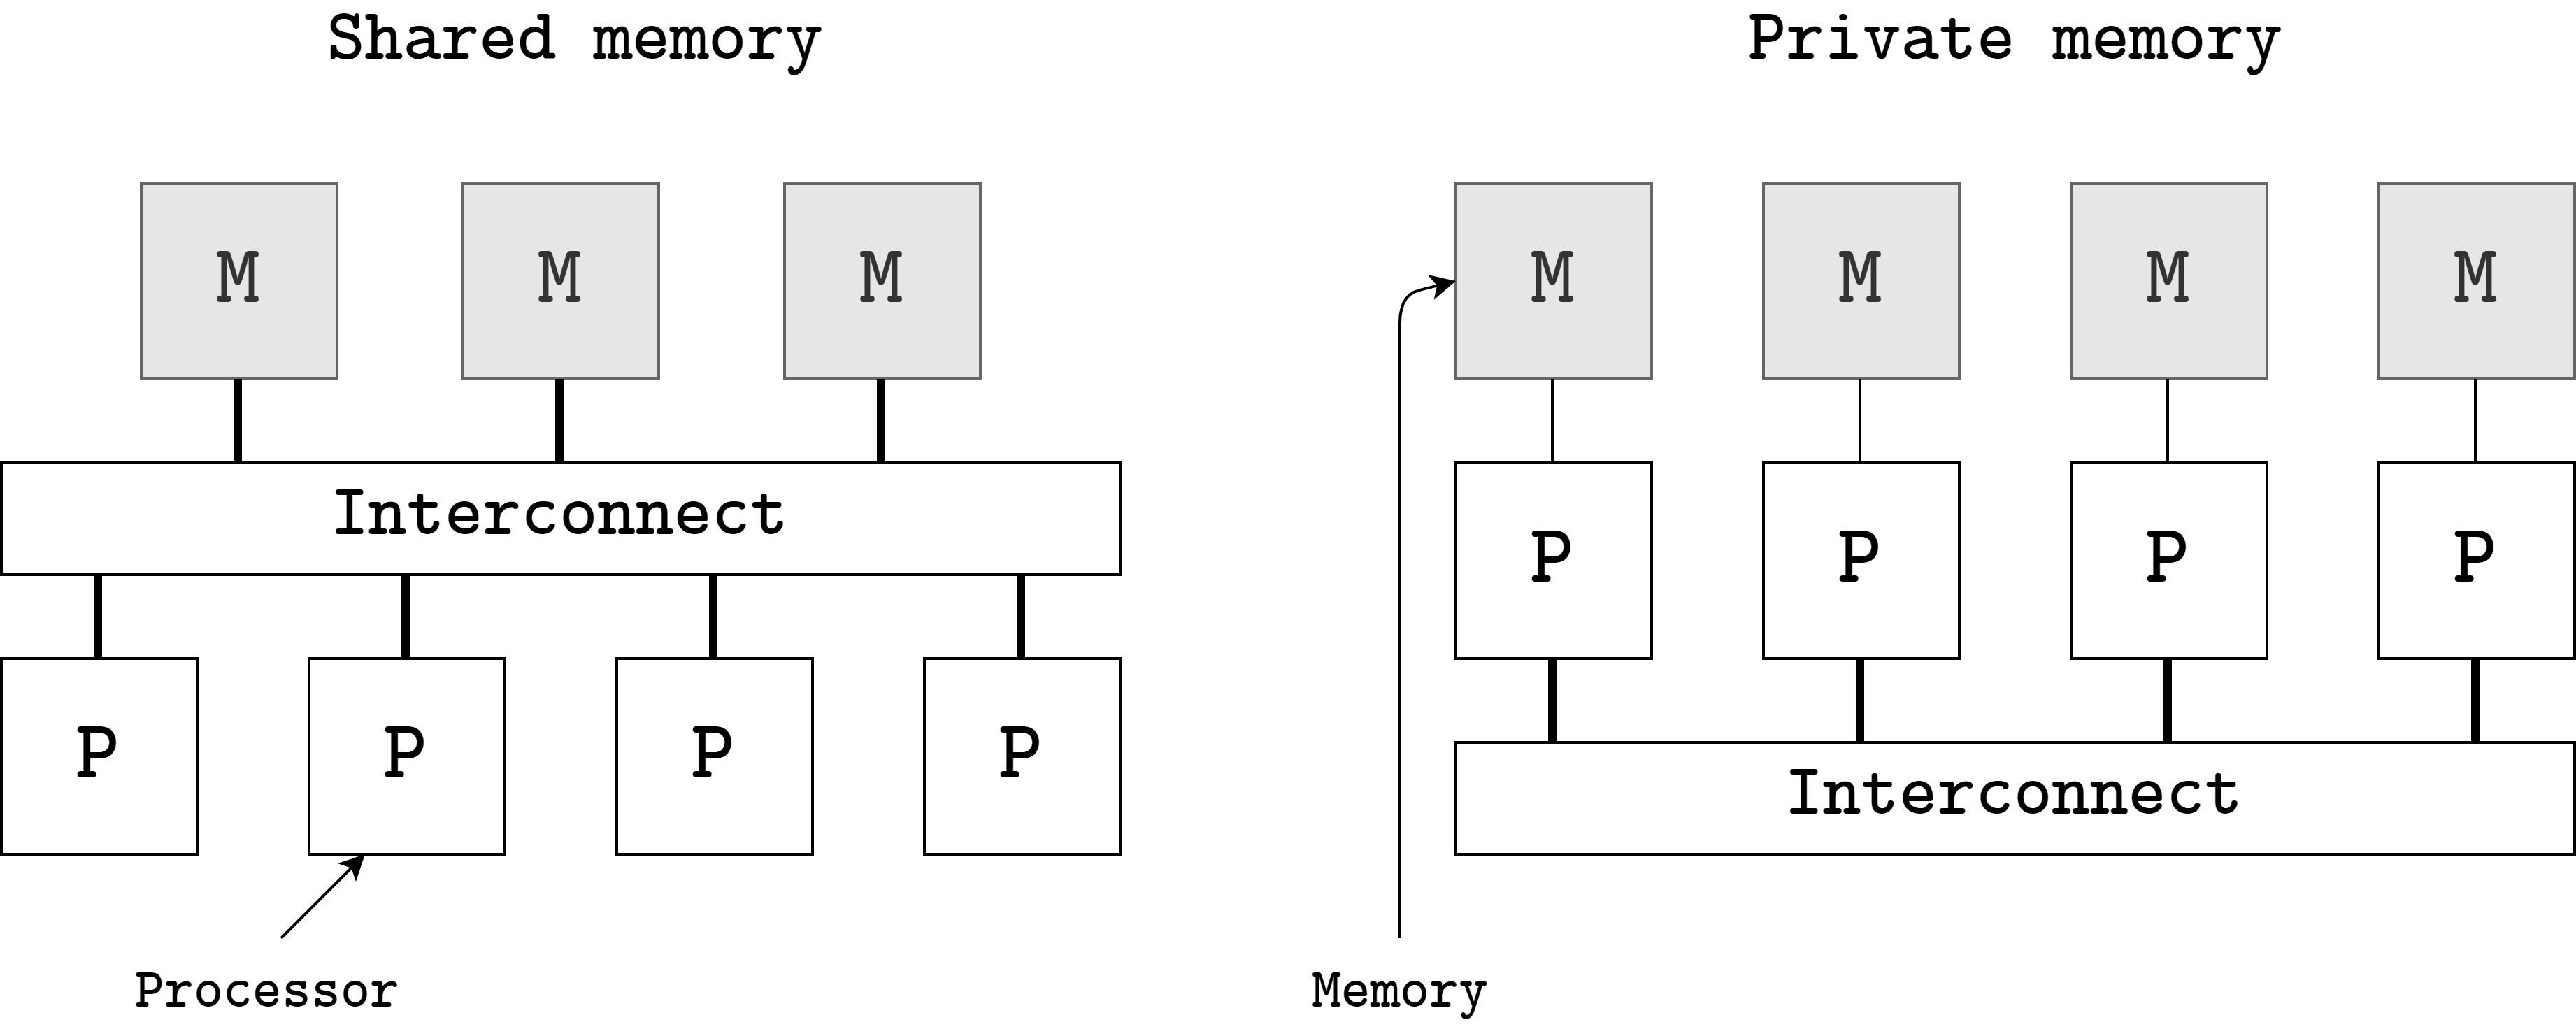
\includegraphics[width=10cm]{./Images/cap2/2.1.png}
    \label{fig:image2.1}
\end{figure}

Molti sistemi distribuiti sono composti da multicomputer eterogenei, con diverse componenti e reti dalle caratteristiche molto diverse. I multiprocessori sono limitati dalla dislocazione geografica, inoltre nella maggior parte dei sistemi distribuiti le operazioni non vengono eseguite in modo transazionale.

\subsection{Algoritmi distribuiti}
Un algoritmo distribuito è la specifica delle azioni che devono essere intraprese dai processi che compongono il sistema, per il raggiungimento di un obiettivo.
Dato che risulta difficile descrivere tutti gli stati possibili di un algoritmo distribuito, anche per via dei malfunzionamenti a cui sono soggetti i processi e la trasmissione dei messaggi, la progettazione di un algoritmo distribuito deve basarsi sulle ipotesi che è possibile fare sulla tempificazione del sistema, e prevedere la gestione dei malfunzionamenti (per quanto possibile).

\subsection{Sistemi distribuiti sincroni}
Un sistema distribuito è sincrono se esistono e sono noti i limiti inferiori e superiori al tempo di esecuzione di ogni passo di elaborazione. In particolare, devono essere noti il limite superiore al tempo di consegna di un messaggio (detto tempo di timeout) e il limite superiore al tasso di deviazione di ciascun clock locale (\textit{clock drift rate}) rispetto al tempo reale.

Spesso è possibile stimare i limiti al tempo di esecuzione dei processi, al ritardo dei messaggi e alla deriva degli orologi, ma è difficile individuare i valori reali. Se non è possibile garantire valori limite, un qualsiasi algoritmo basato su di essi non è affidabile. Per i sistemi sincroni è possibile definire algoritmi distribuiti basati sull'individuazione dei fallimenti tramite timeout, tuttavia è difficile assicurare tramite proprietà in un sistema su grande scala e nel tempo. 

Tipicamente i sistemi distribuiti reali non sono sincroni, ma è comunque possibile costruire sistemi distribuiti sincroni. Infatti se i processi che non possono essere modellati come sincroni hanno limiti superiori probabilistici sui tempi di esecuzione e di comunicazione, è possibile utilizzare i timeout per fare in modo che il sistema si comporti come un sistema parzialmente sincrono. Per fare ciò è necessario individuare le risorse richieste dai processi per eseguire le elaborazioni e per scambiare messaggi, garantire un numero sufficiente di cicli di processore e una sufficiente capacità di rete.

\subsection{Sistemi distribuiti asincroni}
Un sistema distribuito è asincrono se non esistono limiti alla velocità di esecuzione dei processi, al ritardo di trasmissione dei messaggi, o alla deviazione del clock. In un sistema asincrono, non è possibile formulare ipotesi temporali relativamente all'elaborazione, allo scambio messaggi e alla sincronizzazione. 
\begin{mdframed}[backgroundcolor=gray!20,shadow=false]
\textbf{N.B.} I modelli sincrono e asincrono sono gli estremi di uno spettro di possibilità con cui modellare i sistemi reali.
\end{mdframed}

\subsection{Modello dei fallimenti}
Per \textbf{fallimento}(\textit{failure}) si definisce un qualsiasi scostamento da un comportamento considerato corretto o desiderabile. Bisogna però introdurre anche i termini di \textbf{guasto} ed \textbf{errore}.
Un guasto (\textit{fault}) è considerata la causa originaria del fallimento (ad esempio un bug); anche se presente, il fault può non essere attivato in un'esecuzione ma in altri modi. Nel primo caso si dice \textbf{attivo}(\textit{active}), altrimenti è \textbf{dormiente}(\textit{dormant}).

L'errore (\textit{error}) è lo stato in cui transita il sistema a seguito dell'attivazione di un guasto, nel quale dunque il suo comportamento si discosta da quello considerato corretto. Spesso si parla di catena \textit{fault-error-failure}, come si può vedere dall'immagine seguente.

\begin{figure}[ht]
    \centering
    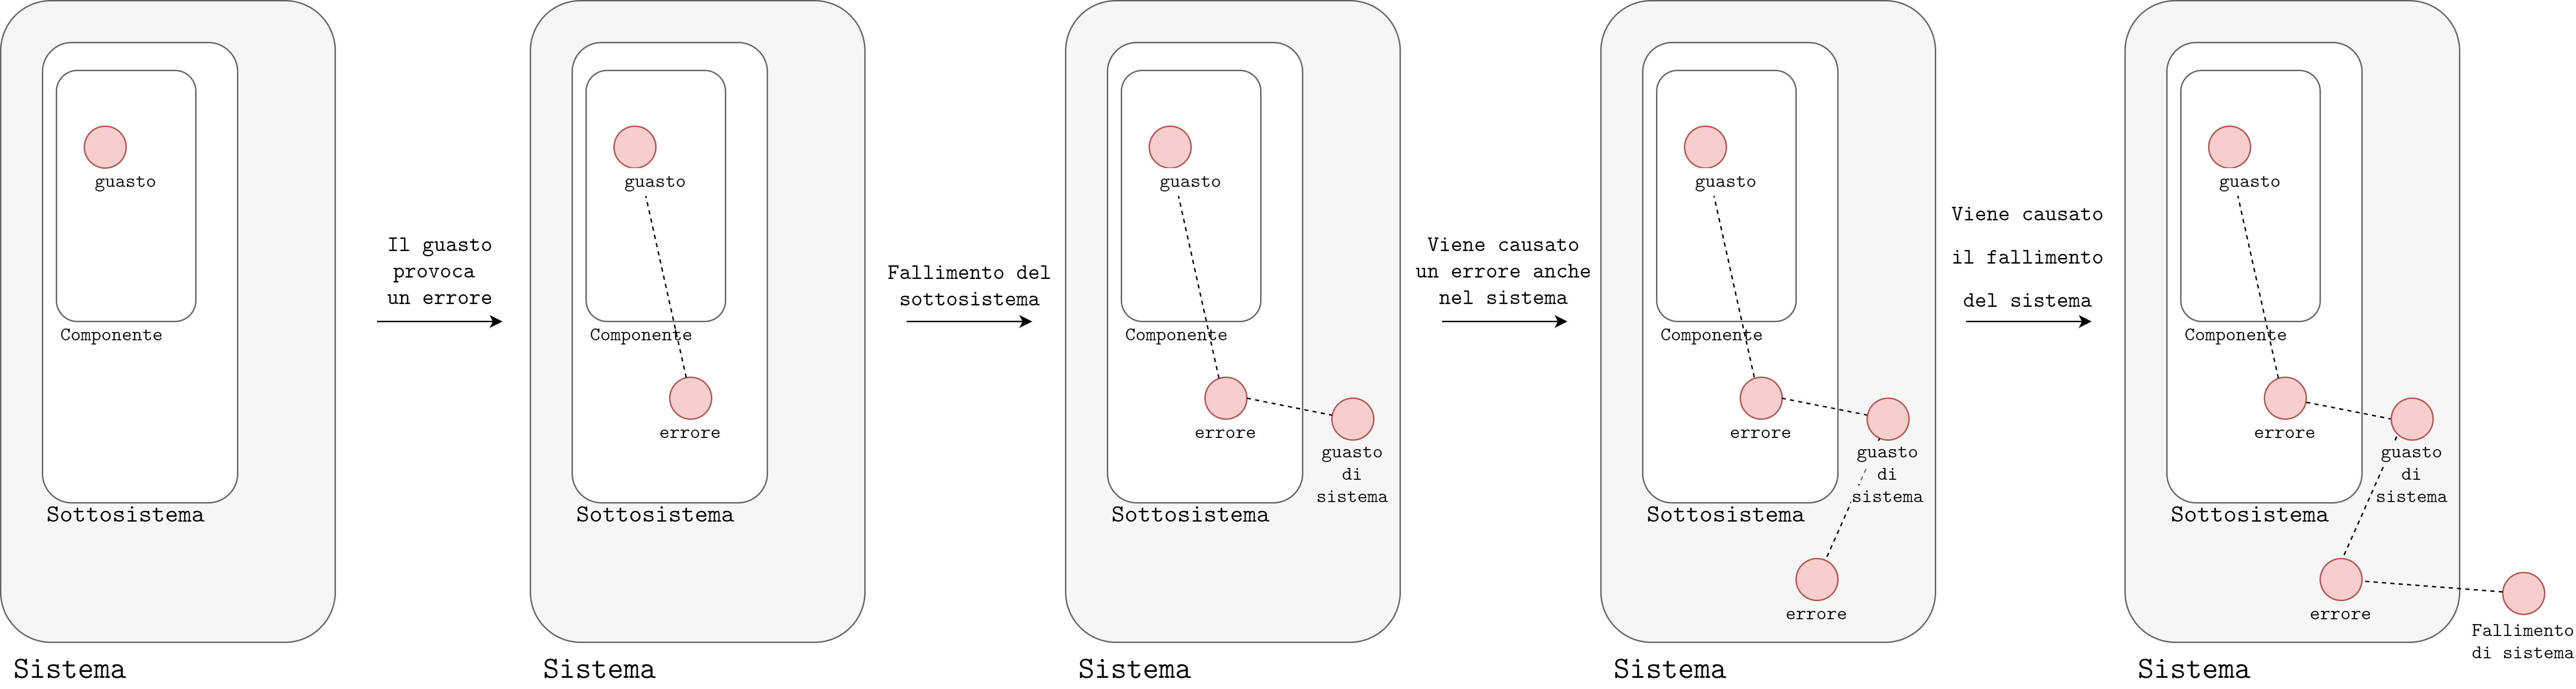
\includegraphics[width=14cm]{./Images/cap2/2.2.png}
    \label{fig:image2.2}
\end{figure}

Un modello dei fallimenti per un sistema distribuito definisce le modalità con cui si possono verificare guasti in processi e canali di comunicazione. I fallimenti possono essere di natura diversa: per crash, per omissione, di valore, bizantini, e in particolare si dividono in:
\begin{itemize}
    \item \textbf{omission failure}: si ha quando un processo o un canale non eseguono un'azione che ci si aspetta che eseguano;
    \item \textbf{timing failure}: mancato rispetto di una scadenza (applicabile solo ai sistemi sincroni);
    \item \textbf{fail stop}: si ha quando un processo non esegue più azioni, e gli altri processi sono in grado di rilevarne il fallimento;
    \item \textbf{crash}: si ha quando un processo non esegue più azioni, e gli altri processi non sono in grado di rilevarne il fallimento;
    \item \textbf{omissione}: può essere da parte di un canale, quando questo non trasporta messaggi, oppure da parte di un processo, nel quale il processo fa una \texttt{send} o una \texttt{receive} ,a il messaggio non viene spedito/ricevuto (\textit{send omission/receive omission});
    \item \textbf{prestazionale}:
    \begin{itemize}
        \item di un canale: il tempo di consegna di un messaggio eccede il limite superiore;
        \item di un processo: il tempo di esecuzione di un'azione eccede il limite superiore;
        \item del clock: la discrepanza rispetto a un clock ideale eccede il limite superiore. 
    \end{itemize}
    \item \textbf{fallimento bizantino}: è la semantica peggiore per un guasto, in cui si può verificare qualunque tipo di errore. Rappresenta un fallimento di un processo o di un canale che si comportano in modo arbitrario, ad esempio mandando più messaggi, omettendo azioni o comportandosi in modo malizioso.
\end{itemize}
\subsection{Modello di sicurezza}
Il modello di interazione prevede processi che incapsulano risorse e forniscono ad altri processi l'accesso ad esse mediante interazioni con scambio di messaggi.

Questo modello quindi è la base per il modello di sicurezza: la sicurezza di un sistema distribuito può essere ottenuta rendendo sicuri i processi e i canali di comunicazione tra essi, e proteggendo le risorse che i processi incapsulano.

La sicurezza nei sistemi distribuiti deve riguardare tutti i componenti del sistema e coinvolge due aspetti principali:
\begin{itemize}
    \item le comunicazioni tra utenti e processi, che ha come soluzione la costruzione di canali sicuri;
    \item l'autorizzazione di utenti e processi, che si può risolvere con un controllo degli accessi.
\end{itemize}
Inoltre un sistema distribuito sicuro ha bisogno di una politica di sicurezza che definisca le azioni che le entità del sistema possono eseguire e quelle che sono proibite. Una politica può essere realizzata tramite meccanismi di sicurezza, come crittografia, autenticazione, autorizzazione.

Le minacce alla sicurezza rientrano in tre grandi classi:
\begin{itemize}
    \item perdita: si riferisce all'acquisizione di informazioni da parte di destinatari non autorizzati;
    \item manomissione: si riferisce all'alterazione non autorizzata delle informazioni;
    \item vandalismo: si riferisce all'interferenza con il corretto funzionamento di un sistema senza guadagno per l'autore.
\end{itemize}
I meccanismi di sicurezza nei sistemi distribuiti sono generalmente posti a livello middleware, in quanto non è nota a priori l'architettura sottostante, essendo un sistema distribuito.
Le dipendenze tra servizi di sicurezza portano al concetto di \textbf{Trusted Computing Base}(TCB), ovvero l'insieme di tutti i meccanismi di sicurezzza in un sistema distribuito che sono necessari per rispettare la sicurezza del sistema. I servizi di sicurezza possono essere isolati da altri tipi di servizi, riducendo la TCB ad un piccolo sottoinsieme di nodi.

\section{Il consenso nei sistemi distribuiti}
Informalmente, il problema del consenso distribuito consiste nel far sì che alcuni processi convengano su un valore, dopo che almeno uno di esse ha effettuato una proposta riguardo tale valore. In pratica:
\begin{itemize}
    \item $N$ processi comunicanti tramite scambio messaggi;
    \item i canali di comunicazione sono affidabili;
    \item i processi sono soggetti a fallimenti di tipo crash oppure bizantini;
    \item il processo $p_{i} (i=1 ... N)$ possiede una variabile di decisione $d_{i}$ e propone un proprio valore $v_{i}$ appartenente ad un insieme $D$;
    \item ciascun processo parte da uno stato di indecisione, e mira a raggiungere uno stato di decisione, in cui il valore di $d_{i}$ è immutabile.
\end{itemize}

Un esempio con tre processi: \newline
- I processi $p_{1}$ e $p_{3}$ propongono di provedere ad un'azione comune; \newline
- Il processo $p_{2}$ propone di abortire l'azione comune, ma poi subisce un crash.

\begin{figure}[ht]
    \centering
    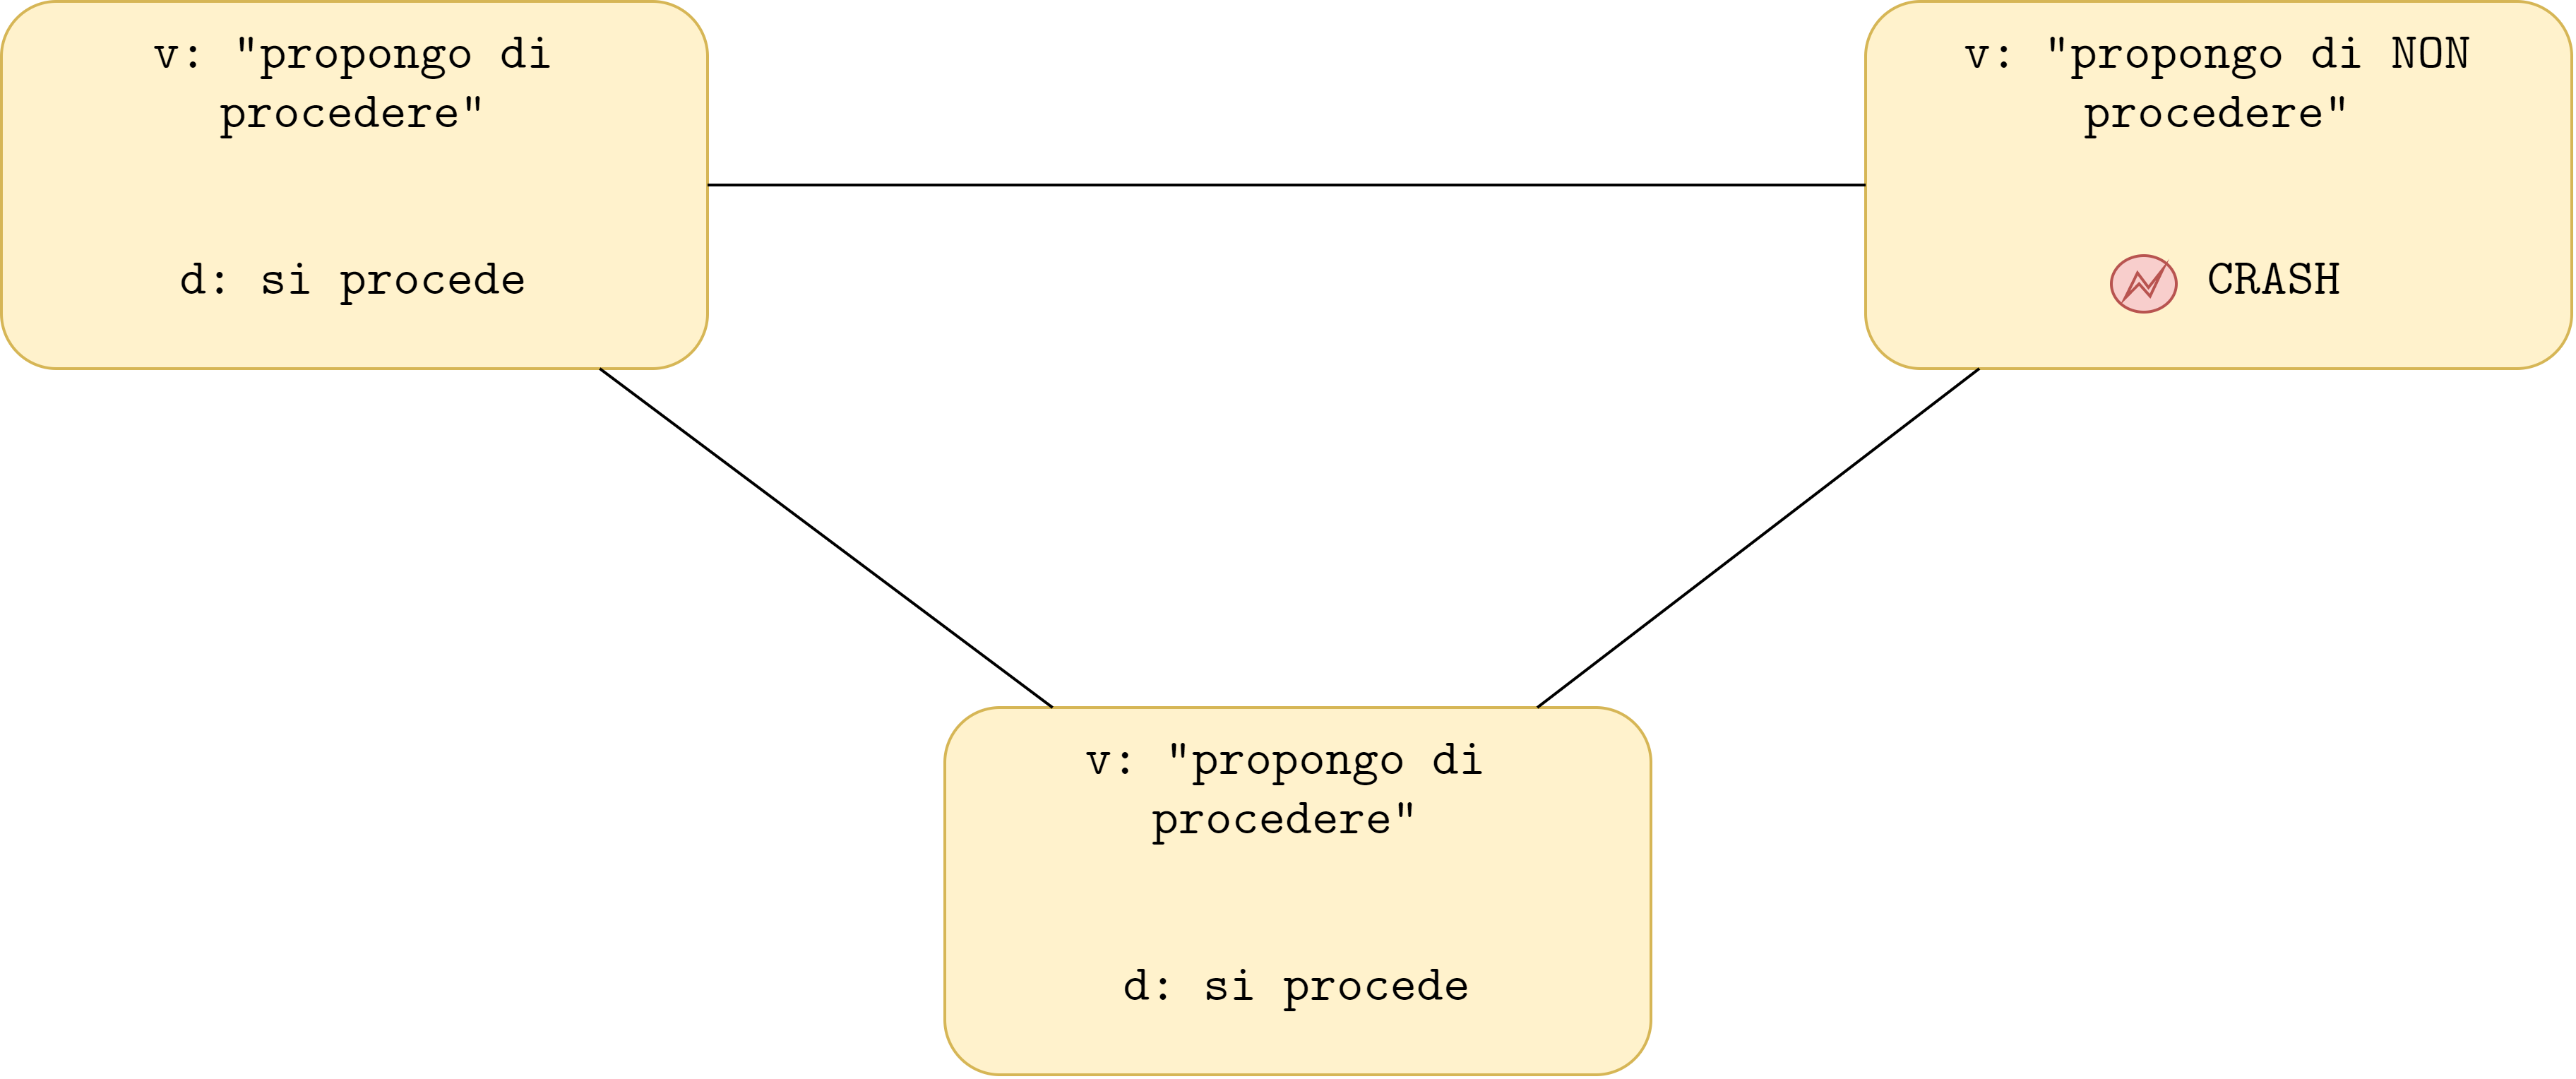
\includegraphics[width=8cm]{./Images/cap2/2.3.png}
    \label{fig:image2.3}
\end{figure}

Un algoritmo di consenso distribuito fa sì che i due processi corretti decidano di procedere. Il processo $p_{2}$ non viene proprio considerato perché è andato in crash e gli altri due processi non se ne sono accorti.

I requisiti che devono essere soddisfatti da un algoritmo di consenso distribuito in ogni sua esecuzione sono:
\begin{itemize}
    \item \textbf{Terminazione}: prima o poi ogni processo corretto prende una decisione;
    \item \textbf{Accordo}: due qualsiasi processi corretti non decidono diversamente;
    \item  \textbf{Integrità}: se tutti i processi corretti propongono lo stesso valore, la decisione finale di ogni processo corretto corrisponde a quel valore.
\end{itemize}

Si possono avere varianti al requisito di integrità: per esempio un requisito più debole richiede che il valore di decisione sia proposto da qualche processo corretto, ma non necessariamente da tutti i processi corretti.

\subsection{Il problema dei generali bizantini}
Nella formulazione informale di Lamport, tre o più generali devono convenire se sferrare un attacco o ritirarsi. Uno di essi è il comandante, gli altri sono i suoi generali.
\begin{itemize}
    \item Il comandante invia l'ordine di attaccare o ritirarsi; i generali devono convenire se attaccare o ritirarsi.
    \item Uno o più generali possono essere maliziosi.
    \item Se il comandante è malizioso, invia ordini diversi ai generali.
    \item Se un generale è malizioso, dice ad alcuni suoi pari che il comandante ha ordinato di attaccare, ad altri che ordinato di ritirarsi.
\end{itemize}

L'attacco ha successo solo se tutti i generali attaccano e nessuno si ritira. Il problema differisce da quello del consenso in quanto non tutti i processi che devono raggiungere l'accordo propongono un valore, ma uno specifico processo (il generale) fornisce loro un valore sul quale devono convenire. Inoltre tipicamente si assume che i generali siano soggetti a fallimenti bizantini, sebbene il problema possa essere posto anche solo con riferimento a fallimenti per crash. \newline
I requisiti del problema dei generali bizantini sono:
\begin{itemize}
    \item Terminazione: prima o poi ogni processo corretto prende una decisione;
    \item Accordo: due qualsiasi processi corretti non decidono diversamente;
    \item Integrità: se il comandante è corretto, tutti i processi corretti decidono per il valore proposto dal comandante.
\end{itemize}

Nel problema dei generali bizantini l'integrità implica l'accordo se il comandante è corretto. 
\subsection{Il problema della consistenza interattiva}
Variante del problema del consenso, nella quale ogni processo propone un solo valore, e l'obiettivo è che tutti i processi concordino su un vettore di valori, uno per ciascuno di essi. I requisiti sono:
\begin{itemize}
    \item Terminazione: prima o poi ogni processo corretto prende una decisione;
    \item Accordo: il vettore di decisione è lo stesso per tutti i processi corretti.
    \item Integrità: se $p_{i}$ è corretto, tutti i processi corretti decidono per il valore $v_{i}$ proposto da $p_{i}$ come elemmento i-esimo del vettore.
\end{itemize}
\subsection{Consenso in un sistema sincrono}
Un algoritmo di consenso basato su multicast. Le ipotesi sono:
\begin{itemize}
    \item Il sistema è sincrono;
    \item Ci sono $N$ processi;
    \item Al più $f$ processi esibiscono fallimenti per crash;
    \item Si dispone di una primitiva \textit{basic multicast} che garantisce che i processi destinatari corretti ricevano il messaggio, finché il mittente (multicaster) non fallisce:
    \begin{itemize}
        \item \texttt{multicast(g, m)} invia il messaggio \texttt{m} a un gruppo \texttt{g} di processi; \texttt{m} porta con sé un identificativo del mittente, e un identificativo del gruppo \texttt{g};
        \item \texttt{deliver(m)} consegna al chiamante il messaggio \texttt{m};
        \item i processi non mentono su origine e destinazione dei messaggi.
    \end{itemize}
    \item $v_{i}^{k}$ è il vettore dei valori proposti noti al processo $p_{i}$ all'inizio del ciclo $k$;
    \item $f+1$ è il numero complessivo di interazioni.
\end{itemize}

Nel caso peggiore, nelle $f+1$ interazioni si verifica il numero massimo crash possibili $f$: l'algoritmo garantisce che al termine i processi corretti sopravvissuti raggiungano il consenso.
Nell'iterazione $k$, il processo $p_{i}$:
\begin{itemize}
    \item invia (B-multicast) i valori che non ha inviato nei cicli precedenti;
    \item riceve (B-deliver) i messaggi analoghi e aggiorna $v_{i}^{k}$ con i nuovi valori ricevuti.
\end{itemize}

Dopo $f+1$ cicli, ogni processo sceglie il valore minimo di $v_{i}^{f+1}$ come valore di decisione.

La durata di un ciclo è limitata da un apposito \textit{timeout}.

\vspace{5mm}

\begin{lstlisting}
Inizializzazione:
    v_{i}^{0} = {};
    v_{i}^{1} = {v_{i}};

k-esima iterazione, 1 <= <= f+1:   (f+1 cicli)
    B-multicast(v_{i}^{k} - v_{i}^{k-1});
    v_{i}^{k+1} = v_{i}^{k};
    while (in iterazione k) {
        B-deliver(v_{j}) da un processo p_{j};
        v_{i}^{k+1} = v_{i}^{k+1} U v_{j};
    }
Dopo f+1 iterazioni:
    d_{i} = minimo(v_{i}^{f+1};
\end{lstlisting}

\vspace{5mm}

I requisiti sono:
\begin{itemize}
    \item Terminazione: ovvia, il sistema è sincrono.
    \item Accordo e integrità: sono raggiunti se si dimostra che tutti i processi sopravvissuti pervengono allo stesso vettore al termine dell'argoritmo, in quanto poi tutti applicano la stessa funzione (calcolo del minimo).
\end{itemize}
\textbf{Dimostrazione}: assumiamo che due processi non abbiamo lo stesso vettore finale, ad esempio che $p_{i}$ abbia un valore $v$ che $p_{j}$ non possiede (con $i \neq j$).

L'unica spiegazione possibile è che $v$ sia stato inviato da un altro processo $p_{k}$ a $p_{i}$ e poi $p_{k}$ sia andato in crash prima di inviarlo a $p_{j}$.

Ma se $p_{k}$ possedeva il valore $v$ senza che $p_{j}$ lo possedesse anch'esso già a conclusione del ciclo precedente, vuol dire che ci deve essere stato nel ciclo precedente un altro processo ancora che ha inviato $v$ a $p_{k}$ ed è andato in crash prima di inviarlo a $p_{j}$.

Iterando il ragionamento, ci deve essere stato almeno un crash per ciclo. Ma ci sono al più $f$ guasti e $f+1$ cicli, è l'ipotesi di assurdo è contraddetta.

Il risultato è generalizzabile (Dolev e Strong, 1983):
\begin{center}
{\textbf{Ogni algoritmo di consenso distribuito che voglia tollerare $f$ fallimenti richiede almeno $f+1$ cicli.}}
\end{center}
\vspace{5mm}

Ne segue che tale limite inferiore si applica anche agli altri di \textit{agreement} distribuito, come quello dei generali bizantini.

\subsection{Comportamento bizantino}
Un difetto bizantino è una condizione di un sistema distribuito in cui i componenti possono guastarsi e c'è imperfetta conoscenza sull'eventuale guasto di un componente. Il termine prende il nome dal problema dei generali bizantini, che descrive una situazione in cui, per evitare un fallimento catastrofico del sistema, gli attori devono concordare una strategia, ma alcuni sono inaffidabili.

In un errore bizantino, un componente può apparire incoerentemente sia guasto che funzionante ai sistemi di rilevamento degli errori, presentando sintomi diversi a diversi osservatori. È difficile dichiararlo guasto ed escluderlo dalla rete, perchè devono prima raggiungere un consenso su quale componente ha fallito per primo. Il comportamento bizantino è sempre un fallimento. Non si riesce a capire che uno dei nodi è fallito e quale, e ad alcuni può addirittura apparire come funzionante. L'output del comportamento bizantino è completamente a caso. Comunque, non potendo avere una rilevazione precisa del fallimento questo non può essere escluso, ma anzi deve essere tollerato. Tuttavia i fallimenti sono arbitrari, non sono ad hoc per far fallire il sistema.
\subsubsection{PROBLEMA CON TRE GENERALI}
Nella variante del problema con tre generali, si ipotizzano due scenari. Si assume che il sistema sia sincrono, e che i canali siano privati (se i processi potessero ispezionare i messaggi degli altri processi, potrebbero riconoscere il processo bizantino). I processi in rosso sono bizantini.

\begin{figure}[ht]
    \centering
    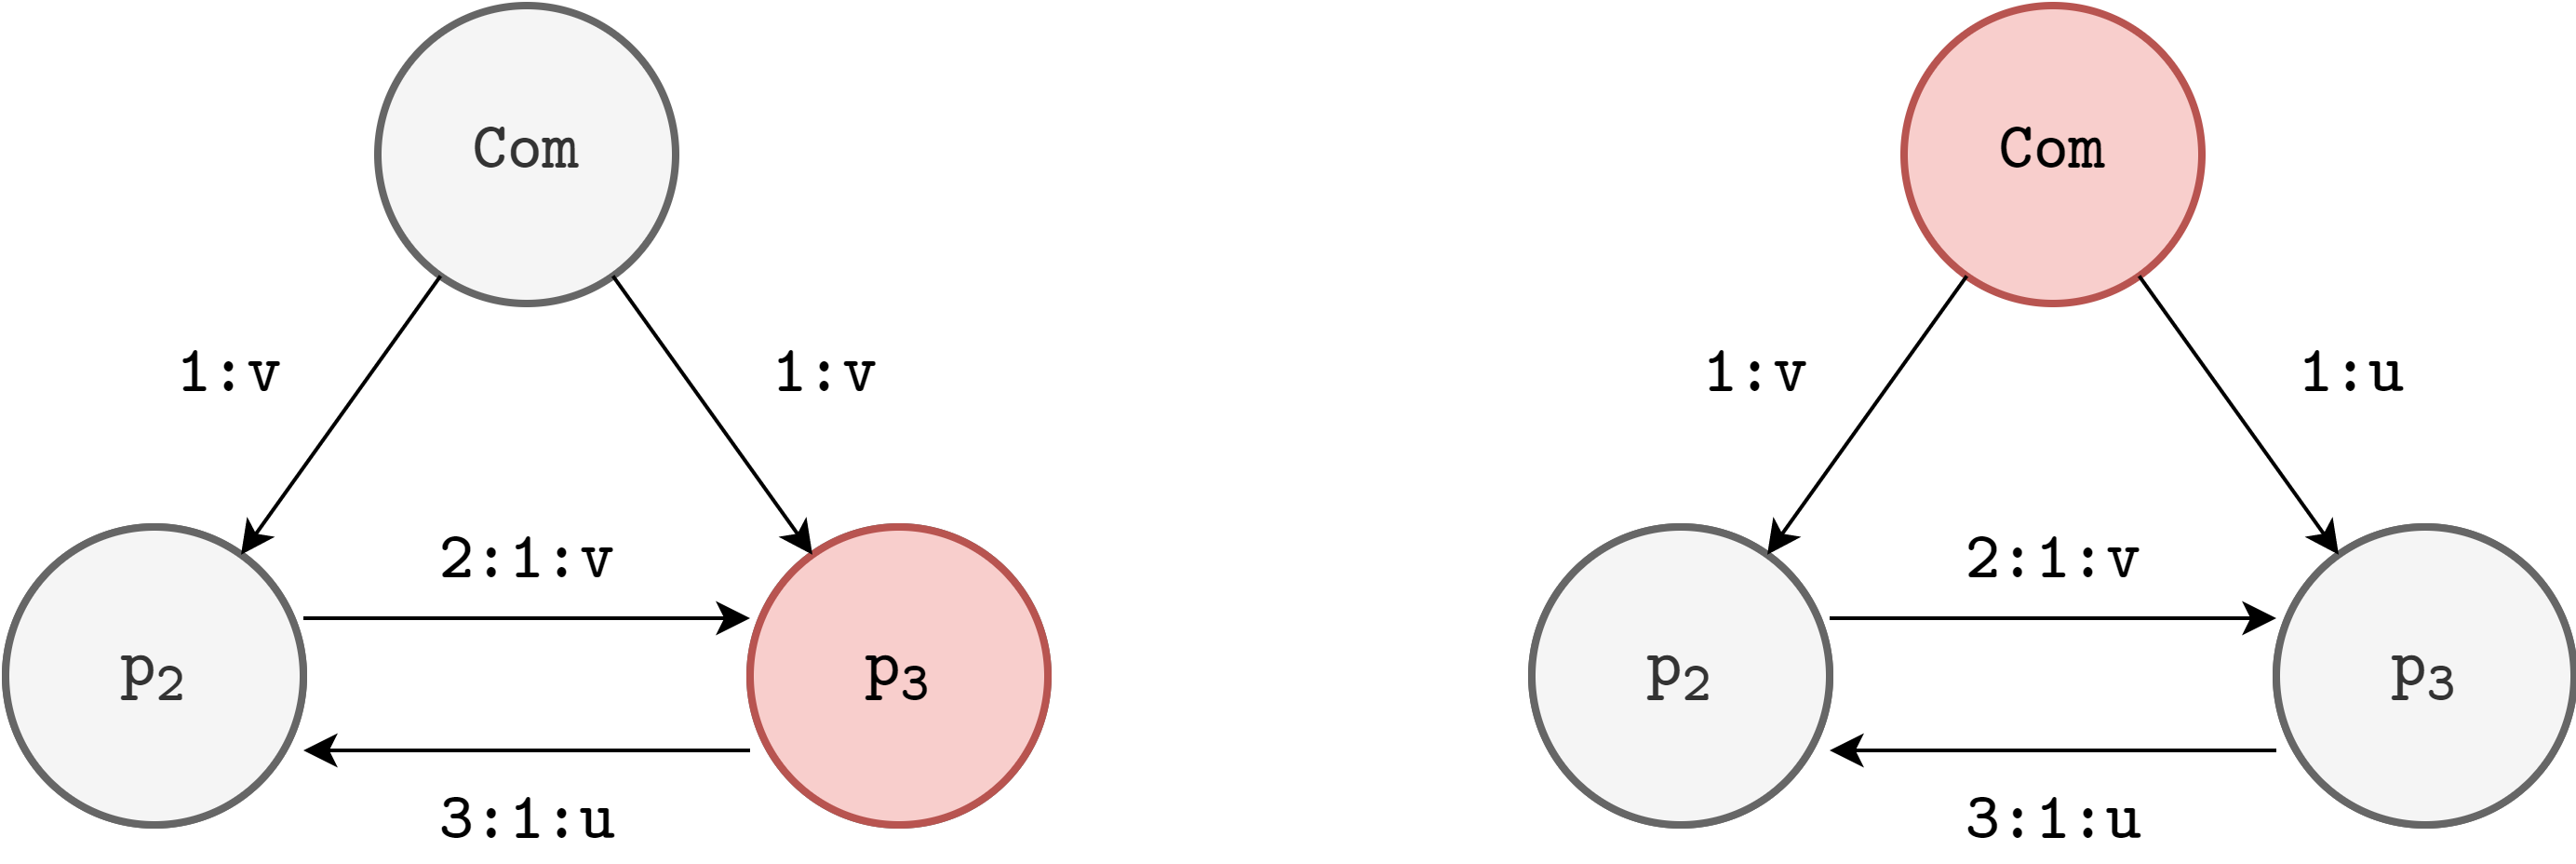
\includegraphics[width=9cm]{./Images/cap2/2.4.png}
    \label{fig:image2.4}
\end{figure}

\begin{itemize}
    \item Supponiamo che p3 sia bizantino. Il comandante invia $v$ sia a $p_{2}$ che a $p_{3}$, ma $p_{3}$ invia $u$ a $p_{2}$, mentre quest'ultimo invia correttamente $v$. Il processo $p_{2}$ si trova nella situazione in cui riceve due valori diversi, e non può capire chi è compromesso tra $p_{2}$ e il comandante.
    \item Supponiamo invece che il comandante sia bizantino, e invia $v$ a $p_{2}$ e $u$ a $p_{3}$. Questi ultimi si scambiano correttamente i valori, ed entrambi si trovano nella situazione in cui devono capire se l'altro processo o il comandante sono compromessi. Ovviamente anche in questo caso non c'è soluzione.
\end{itemize}
Se esistesse una soluzione, per il requisito di integrità $p_{2}$ dovrebbe scegliere il valore $v$ fornito dal comandante se questo è corretto. Ma nei due casi, $p_{2}$ è nella stessa situazione. Per simmetria si ha che se $p_{3}$ è corretto, deve scegliere il valore del comandante. Ma ciò viola la condizione di \textit{agreement}. perché se il comandante è faulty invia valori diversi ai due luogotenenti. \newline
\textbf{In generale, non esiste soluzione se $N \leq 3f$.}
\subsubsection{PROBLEMA CON QUATTRO GENERALI}
Nel caso invece ci siano 3 luogotenenti e un comandante, la situazione cambia, come è possibile vedere dall'immagine seguente. Infatti si ha che:
\begin{itemize}
    \item $p_{2}$ per maggioranza (v, u, v) = v
    \item $p_{4}$ per maggioranza (v, v, w) = v
    \item $p_{1}$, $p_{2}$, $p_{3}$ per maggioranza non convengono a nessun valore, anzi a un valore nullo, che poi non viene considerato\footnote{A volte al posto del simbolo dell'insieme vuoto viene utilizzata una T rovesciata, che indica la mancanza di informazioni.}: maggioranza (u, v, w) = Ø
\end{itemize}

\begin{figure}[ht]
    \centering
    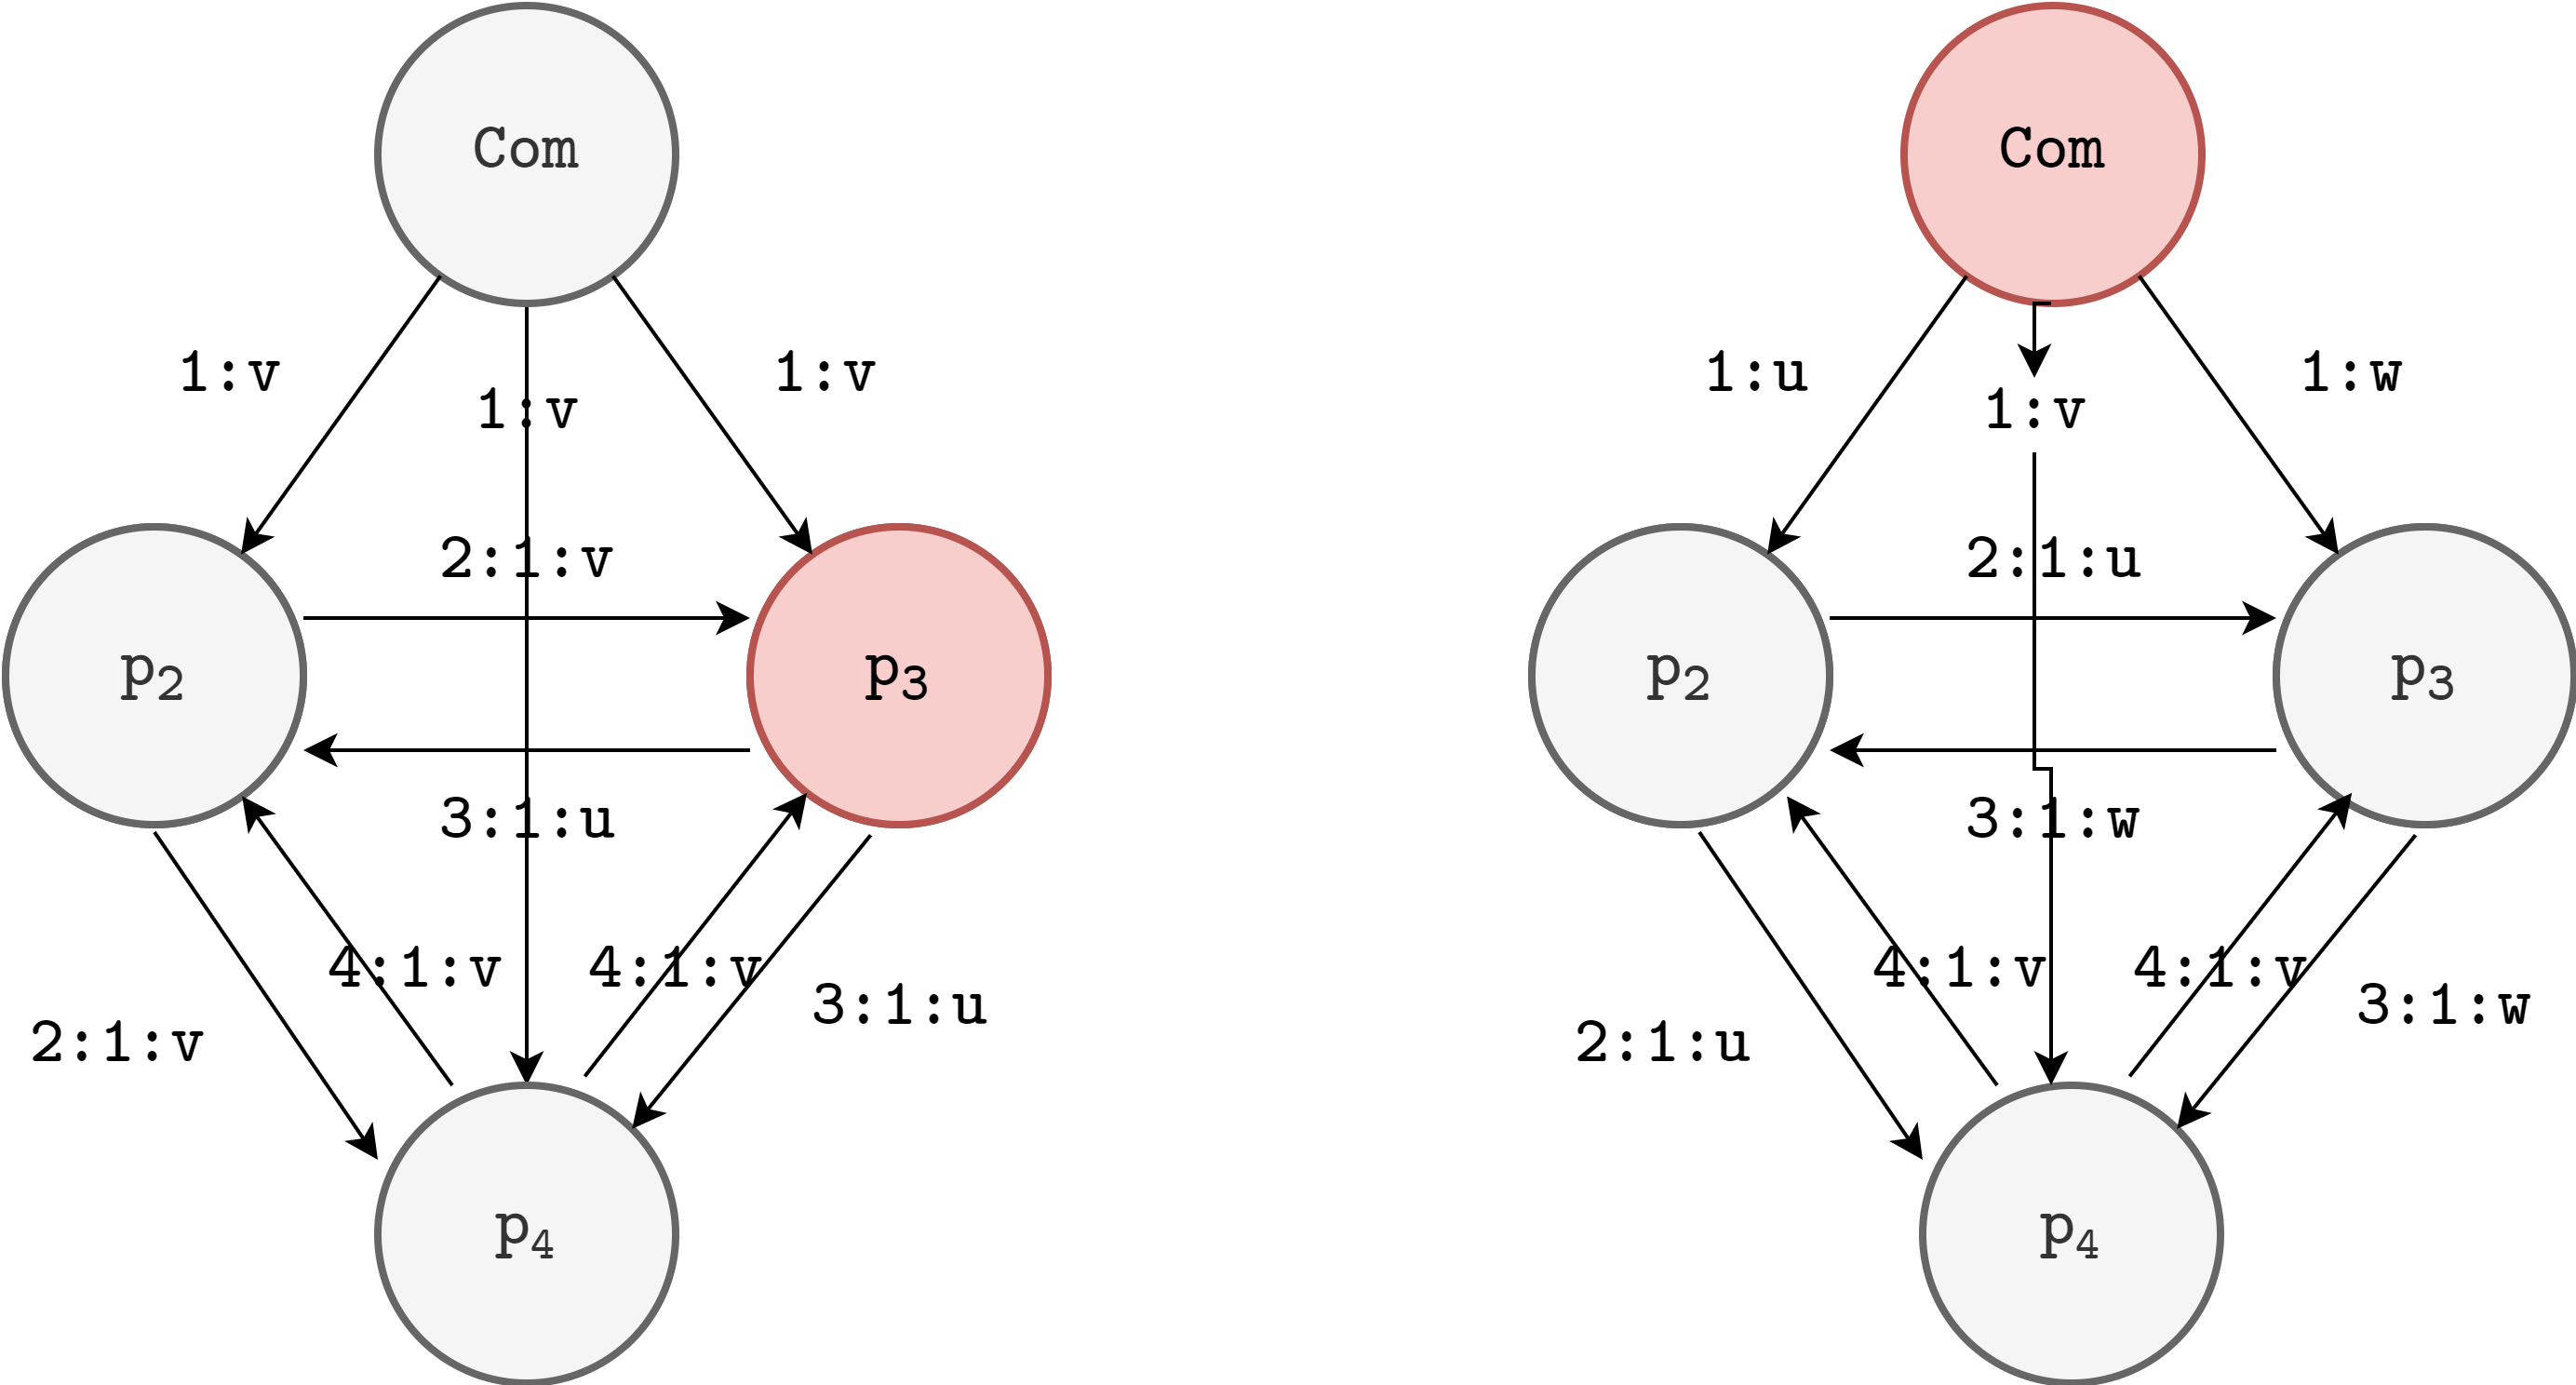
\includegraphics[width=9cm]{./Images/cap2/2.5.png}
    \label{fig:image2.5}
\end{figure}

\subsection{Consenso nei sistemi asincroni}
Non esiste alcun algoritmo deterministico in grado di garantire il raggiungimento del consenso in un sistema asincrono a scambio di messaggi nel caso di anche un solo fallimento per \textit{crash} di un processo. (Fischer, Lynch, Paterson).

Di conseguenza, non esistono soluzioni garantite in un sistema asincrono per il problema dei generali bizantini e per quello della consistenza interattiva. Tuttavia, si può forzare la garanzia di ottenere il consenso, basta indebolire: 
\begin{itemize}
    \item \textbf{la condizione di Termination}: introducento elementi di non determinismo oppure garantendo la termination esclusivamente durante periodi di sincronia del sistema.
    \item \textbf{la condizione di Agreement}: individuando un insieme finito per i possibili valori decisionali dei singoli processi.
    \item \textbf{il modello del sistema}: introducendo dei \textit{failure detectors} per distinguere i processi lenti (ma corretti) da quelli effettivamente falliti.
\end{itemize}

\begin{table}[ht]
\begin{tabular}{|l|l|l|}
\hline
\textbf{Metodo di fallimento} & \textbf{Sistema sincrono}                                                                                                        & \textbf{Sistema asincrono}                                                                             \\ \hline
Nessuno                       & \begin{tabular}[c]{@{}l@{}}Consenso ottenibile\\ Conoscenza comune ottenibile\end{tabular}                                       & \begin{tabular}[c]{@{}l@{}}Consenso ottenibile\\ Conoscenza comune concorrente \\ ottenibile\end{tabular} \\ \hline
Crash                         & \begin{tabular}[c]{@{}l@{}}Consenso ottenibile per f < n processi \\ non corretti con $\Omega(f+1)$ cicli\end{tabular}      & Consenso non ottenibile                                                                                \\ \hline
Bizantino                     & \begin{tabular}[c]{@{}l@{}}Consenso ottenibile per $f \leq (n-1)/3$\\ processi bizantini con $\Omega(f+1)$ cicli\end{tabular} & Consenso non ottenibile                                                                                \\ \hline
\end{tabular}
\end{table}
\subsection{L'algoritmo di Paxos}
Il nome di questo algoritmo deriva dal funzionamento del parlamento dell'isola di Paxos nell'antica Grecia, detto "Parlamento part-time" in quanto funzionava in modo molto particolare:
\begin{itemize}
    \item Ciascun membro aveva un registro in cui annotare tutte i decreti approvati.
    \item I decreti approvati erano numerati (in ordine crescente).
    \item I parlamentari, così come i messaggeri, potevano entrare ed uscire dal parlamento a piacere.
    \item I messaggeri potevano anche uscire prima di consegnare un messaggio affidatogli, “magari per un viaggio di sei mesi” o “andar via per sempre e il messaggio non veniva consegnato".
    \item Ma quando in Camera, parlamentari e messaggeri erano dediti al lavoro ed eseguivano prontamente i loro compiti.
    \item C’era molto rispetto e fiducia tanto che si tendeva a far passare ogni decreto proposto.
    \item Ogni legislatore di Paxos mantneva un libro mastro, dove registrava tutto ciò che è succedeva (con inchiostro indelebile).
    Ciò poneva un problema: se dei parlamentari decretavano che \textit{"37. È proibito dipingere sulle pareti del tempio"} per poi abbandonare il parlamento per un banchetto, un altro gruppo di legislatori appena entrati in parlamento, e ignari di quanto appena deciso, poteva far passare il decreto \textit{"37. È garantita libertà d'espressione artistica"}, in conflitto con il precedente.
    \item I registri di due parlamentari non dovevano contenere informazioni contraddittorie.
\end{itemize}

Per garantire progresso occorreva che almeno la metà dei legislatori fosse in Camera per un tempo sufficientemente lungo. In tal caso, ogni legge proposta da un parlamentare prima o poi era promulgata (ovvero ratificata da una maggioranza di parlamentari). Ogni legge ratificata appariva nel registro di ogni parlamentare.

Ogni parlamentare era fornito di:
\begin{itemize}
    \item un registro sul quale annotare le leggi promulgate;
    \item una penna ad inchiostro indelebile per scrivere sul registro;
    \item tutti i messaggeri di cui necessitava per comunicare col gli altri parlamentari;
    \item una clessidra e fogli di carta secondo necessità.
\end{itemize}
I matematici dell'isola di Paxos elaborarono un complesso sistema per garantire consistenza e progresso al parlamento. Tuttavia questo meccanismo aveva un punto di debolezza relativamente all'elezione dei nuovi membri del parlamento, che avveniva utilizzando le regolari procedure del parlamento. 

Un giorno, a causa di un errore, passò una legge che asseriva che gli unici membri del parlamento erano dei marinai periti in un incidente navale. Da quel momento il parlamento fu abbandonato e la civiltà di Paxos tramontò rapidamente, finché un tiranno prese possesso dell'isola con un colpo di stato instaurando una dittatura militare che pose fine a secoli di progresso governativo.

\vspace{5mm}

Il documento di Paxos specifica che all'interno del parlamento ci sono tre tipi di legislatori: proponenti , accettatori, discenti.
\begin{itemize}
    \item I \textbf{proponenti} (proposer) sostengono le richieste dei cittadini e portano nuove richieste nel parlamento. Un proponente propone un valore sul quale vuole che ci si metta d'accordo, e lo fa con l'invio di una proposta contenente un valore all'insieme di tutti gli accettatori.
    \item Gli \textbf{accettatori} (acceptors) sono i legislatori che votano. Questi decidono se accettare o meno il valore. Ogni acceptor sceglie un valore in modo indipendente e trasmette la sua decisione ai discenti.
    \item I \textbf{discenti} (learner) determinano se un valore è stato accettato. Nell'algoritmo di Paxos, un valore per essere accettato necessita che la maggioranza degli acceptors scelga lo stesso valore.
\end{itemize}
Un certo numero di proposer propone un valore agli acceptors. Quando un acceptor accetta un valore esso invia il risultato ai nodi learners.

Ogni round di successo ha due fasi, cioè i proposer inviano due tipi di messaggi agli acceptors: \texttt{prepare} e \texttt{accept}.
Il proposer propone un decreto al parlamento. Un decreto ha un numero e un valore, il quale può essere qualsiasi cosa, ma è necessario che il numero associato al decreto sia strettamente \textbf{crescente}.
Dopo che un decreto è stato proposto, gli acceptors discutono.

Ora, se il numero legale o la maggioranza dei legislatori votano sì, il decreto passa e tutti lo registrano su i libri. Non appena il \textbf{consenso} è avvenuto, i learners imparano il risultato e poi lasciano il parlamento facendo sapere a tutti gli abitanti dell'isola cosa è successo in parlamento.

\vspace{5mm}

\noindent È ora opportuno fare un parallelismo tra la storia dell'isola di Paxos e i sistemi distribuiti:

\vspace{5mm}

\noindent\textbf{Parlamento} $\rightarrow$ \textbf{Sistema distribuito}\newline
\textbf{Parlamentari} $\rightarrow$ \textbf{Processi}\newline
\textbf{Uscita/entrata dalla camera} $\rightarrow$ \textbf{Fallimento/recovery}\newline
\textbf{Registro} $\rightarrow$ \textbf{Memoria stabile}\newline
\textbf{Messaggeri} $\rightarrow$ \textbf{Comunicazione asincrona tra i processi}\newline

\vspace{3mm}

\noindent I prossimi due capitoli spiegano nel dettaglio il funzionamento dell'algoritmo di Paxos, il primo in un modo più semplice ed intuitivo, il secondo più dettagliato.

\subsection{Funzionamento dell'algoritmo (A)}
Un nodo di Paxos può assume uno solo o tutti e tre i ruoli: \textit{proposer}, \textit{acceptor}, e \textit{learner}. Un proposer propone un valore sul quale vuole che ci si metta d’accordo. Lo fa con l’invio di una proposta contenente un valore a l’insieme di tutti gli acceptors, che decidono se accettare o meno il valore. Ogni acceptor sceglie un valore in modo indipendente – può ricevere più proposte, ognuna da un proposer diverso – e trasmette la sua decisione ai learners, che determinano se un valore è stato accettato. Un valore per essere accettato da Paxos, una maggioranza di acceptors deve scegliere lo stesso valore. Nella pratica, un singolo nodo può assumere molti o tutti questi ruoli, ma negli esempi di questo capitolo, ogni ruolo viene eseguito su un nodo separato, come illustrato di seguito.
\clearpage
\begin{figure}[hbt!]
    \centering
    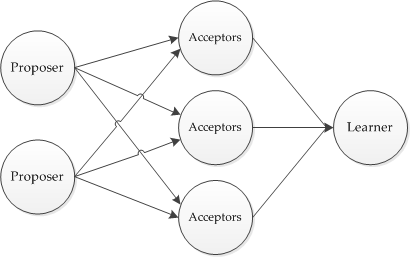
\includegraphics[width=8cm]{./Images/cap2/2.6.png}
    \label{fig:image2.6}
\end{figure}

Nell’algoritmo standard di Paxos, i proposers inviano due tipi di messaggi agli acceptors: \texttt{prepare} o \texttt{accept}. Nella prima fase di questo algoritmo un proposer invia una richiesta di prepare ad ogni acceptor, contentente un valore $v$,  e un numero di round, $n$.

Il valore proposto può essere un qualsiasi valore arbitrario. In questo capitolo i nodi di Paxos stanno cercando di raggiungere un consenso su un valore intero. Il numero di round (anche detto numero della proposta) deve essere positivo, crescente e unico, rispetto al numero di round inviato dagli altri proposers.

Nell’esempio illustrato di seguito, ci sono due proposers, ed entrambi inviano una richiesta di \texttt{prepare}. La richiesta da parte del proposer A raggiunge gli acceptors X e Y prima della richiesta del proposer B, ma la richiesta del proposer B raggiunge l’acceptor Z prima.
\vspace{5mm}

\begin{figure}[ht]
    \centering
    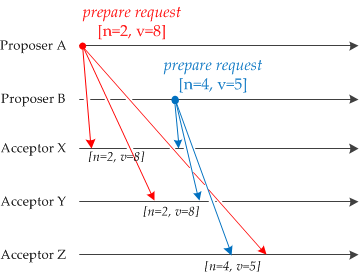
\includegraphics[width=8cm]{./Images/cap2/2.7.png}
    \label{fig:image2.7}
\end{figure}
\vspace{5mm}
Se l’acceptor che ricevere una richiesta di \texttt{prepare} non ha visto un’altra proposta, l’acceptor risponde con una risposta di \texttt{prepare} che promette di non accettare un’altra proposta con un numero di round inferiore. Questo è illustrato nella figura successiva, che mostra le risposte di ciascun acceptor alla prima richiesta di \texttt{prepare} che ricevono.
\clearpage

\begin{figure}[ht]
    \centering
    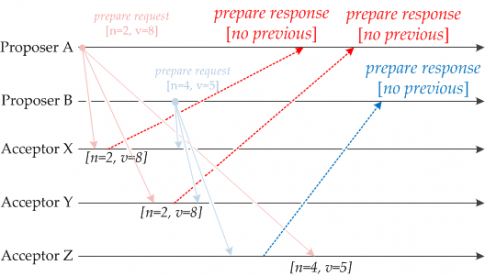
\includegraphics[width=9cm]{./Images/cap2/2.8.png}
    \label{fig:image2.8}
\end{figure}

Alla fine, l’acceptor Z riceve la richiesta dal proposer A, e gli acceptors X e Y ricevono il messaggio dal proposer B. Se l’acceptor ha già visto una richiesta con un numero di round superiore, la richiesta di \texttt{prepare} viene ignorata, come nel caso del proposer A con l’acceptor Z. Se l’acceptor non ha visto una richiesta con un numero di round più alto, prometterà nuovamente di ignorare eventuali richieste con numeri di round più bassi, e rinvia il messaggio precedente con il numero di round più alto che ha visto, insieme al valore di tale proposta. Questo è il caso della richiesta del proposer B e degli acceptors X e Y, come illustrato di seguito:

\begin{figure}[ht]
    \centering
    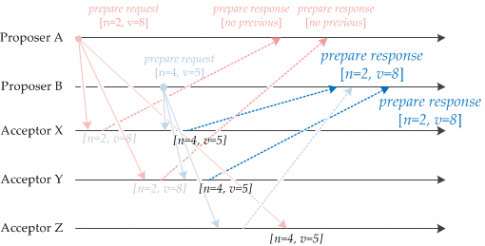
\includegraphics[width=10cm]{./Images/cap2/2.9.png}
    \label{fig:image2.9}
\end{figure}
\FloatBarrier
Una volta che un proposer ha ricevuto delle risposte di \texttt{prepare} da una maggioranza di acceptors, può emettere una richiesta di \texttt{accept}. Siccome il proposer A riceve solo risposte che indicano che non vi erano precedenti proposte,  invia una richiesta di \texttt{accept} ad ogni acceptor con lo stesso numero di round e di valore della proposta iniziale (n=2, v=8). Tuttavia, queste richieste vengono ignorate da ogni acceptor perché hanno tutti promesso di non accettare le richieste con un numero di round inferiore a 4 (in risposta alla richiesta di prepare del proposer B).


\vspace{5mm}

Il proposer B invia una richiesta di \texttt{accept} ad ogni acceptor contenente il numero di round usato in precedenza (n=4) e il valore associato con il più alto numero di round  del messaggio di \texttt{prepare} ricevuto (v=8). Da notare che questo non è il messaggio che il proposer B ha inizialmente proposto, ma il valore più alto che ha visto in precedenza.

\begin{figure}[ht]
    \centering
    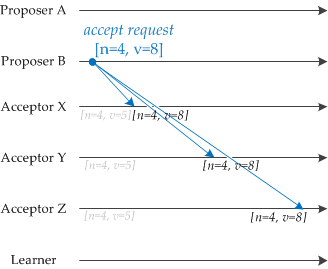
\includegraphics[width=8cm]{./Images/cap2/2.10.png}
    \label{fig:image2.10}
\end{figure}
\FloatBarrier
Se un acceptor riceve una richiesta di \texttt{accept} per un numero di round superiore o uguale  a quello che ha già visto, accetta e invia una notifica ad ogni nodo learner. Un valore è scelto dall’algoritmo di Paxos quando un learner scopre che una maggioranza di acceptors ha accettato un valore, come illustrato di seguito:

\begin{figure}[ht]
    \centering
    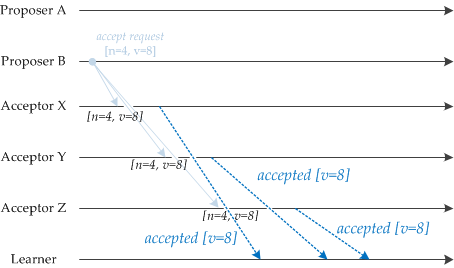
\includegraphics[width=10cm]{./Images/cap2/2.11.png}
    \label{fig:image2.11}
\end{figure}

Una volta che un valore è stato scelto da, un’ulteriore comunicazione con gli altri proposers non può modificare questo valore. Se un altro proposer, il proposer C, invia una richiesta di \texttt{prepare} con un numero di round superiore rispetto a quanto è stato precedentemente visto, e un vlaore diverso (per esempio, n=6, v=7), ciascun acceptor risponde con la precedente proposta più alta (n=4, v =8). Ciò richiede che il proposer C invii una richiesta di \texttt{accept} contentente [n=6, v=8], che conferma solo il valore che è già stato scelto. Inoltre, se qualche minoranza di acceptors non ha ancora scelto un valore, questo processo assicura che alla fine si raggiungerà il consenso sullo stesso valore.

\vspace{5mm}

Vari miglioramenti per aumentare l’efficienza per l’algoritmo standard di Paxos sono discussi nei paper di Lamport and Baker et al.. Ad esempio, una richiesta di prepare non è necessaria se il proposer sa che è il primo a suggerire un valore. La proposta per una richiesta di questo tipo viene numerata come 0 (zero), in modo che sarà ignorata se qualsiasi richiesta numerata con un numero di round più alto è già stata ricevuta.

\subsection{Funzionamento dell'algoritmo (B)}
Innanzitutto illustriamo le proprietà del consenso di Paxos:
\begin{itemize}
    \item \textbf{Liveness}: uno tra i valori proposti prima o poi viene scelto. Se un valore viene scelto, ogni processo prima o poi apprenderà tale scelta.
    \item \textbf{Safety}: un valore può essere scelto solo tra quelli proposti. Il valore scelto deve essere unico. Un processo non deve mai apprendere che un valore è stato scelto a meno che esso non sia stato effettivamente scelto.
\end{itemize}
\subsubsection{RUOLI DEI PROCESSI}
Ogni processo può svolgere uno o più dei seguenti ruoli:
\begin{itemize}
    \item \textbf{Proposer}: svolge tale ruolo un processo che ha la facoltà di proporre un valore.
    \item \textbf{Acceptor}: Svolge tale ruolo un processo che ha la facoltà di accettare un valore precedentemente proposto da un proposer.
    \item \textbf{Learner}: svolge tale ruolo un processo che ha la facoltà di apprendere la scelta di un valore effettuata da un acceptor.
\end{itemize}
Si ricorda che il sistema è asincrono, con processi non bizantini, eseguiti a velocità arbitrarie, che possono fallire per poi riprendere l'esecuzione. Poiché possono fallire dopo che un valore è stato deciso e poi ripartire, è necessario che ricordino alcune informazioni anche dopo un recovery (altrimenti non c'è soluzione). I messaggi non hanno limiti di dimensioni, possono essere duplicati o persi, ma non corrotti.

\subsubsection{SCELTA DI UN VALORE}
Il modo più semplice sarebbe quello di avere un solo acceptor, tuttavia sarebbe un \textit{Single point of failure}: il fallimento dell'acceptor renderebbe impossibile il progresso dell'algoritmo.

Quindi si considera un insieme di acceptor, e un valore proposto è scelto se un insieme sufficientemente grande di essi lo accetta. Si può considerare abbastanza grande una qualunque maggioranza, benché due maggioranze abbiano almeno un acceptor in comune, a condizione però che un acceptor accetti al più un valore.

\vspace{5mm}

In assenza di fallimenti o perdite di messaggi, è desiderabile che un valore venga scelto anche se proposto da un solo proposer. È quindi auspicabile che il seguente requisito sia soddisfatto:\newline
\textbf{P1: Un acceptor deve accettare la prima proposta che riceve.}\newline
Tuttavia, se diversi proposer propongono valori diversi in tempi vicini, il requisito P1 potrebbe portare alla situazione in cui ogni acceptor ha accettato un valore ma nessun valore è scelto da una maggioranza di acceptor. Ad esempio, anche con due soli valori proposti, se ciascuno è accettato da circa la metà degli acceptor, il fallimento di uno potrbbe rendere impossibile apprendere quale è stato scelto.

Quindi P1 e il requisito che un valore sia scelto solo se accettato da una maggioranza di acceptor impongono quindi di ammettere che un acceptor possa accettare più di una valore. Per tener traccia delle diverse proposte accettate si associa ad ogni proposta un numero naturale di serie distinto (n effetti dunque una proposta è una coppia numero di serie - valore ). Un valore viene scelto quando una proposta con quel valore è accettata dalla maggioranza degli acceptor. In tal caso diciamo che la proposta è stata scelta.

Possiamo ammettere che siano scelte proposte differenti, a condizione che contengano lo stesso valore. È sufficiente a tale scopo garantire che: \newline
\textbf{P2: Se viene scelta una proposta con valore v e numero seriale n, allora ogni proposta scelta con numero seriale n' > n deve avere valore v.}\newline
Affinché un valore sia scelto, deve essere accettato da almeno un acceptor. Allora si può soddisfare il requisito P2 richiedendo che:\newline
\textbf{P2\textsuperscript{a}: Se viene scelta una proposta con valore v e numero seriale n, allora ogni proposta con un numero seriale n' > n accettata da un qualsiasi acceptor deve avere valore v.}

La comunicazione asincrona può far si che una proposta sia scelta da un acceptor quando un altro acceptor c non ha ancora ricevuto alcuna proposta. Un nuovo proposer (che si sveglia ignaro all'improvviso) potrebbe allora fare una proposta con un numero di serie maggiore e con valore diverso, e P1 impone che c accetti tale valore (il primo ricevuto da c) violando P2\textsuperscript{a}. 

Mantenere P1 e P2\textsuperscript{a} richiede dunque di restringere il requisito P2\textsuperscript{a}. Si considera allora il requisito più forte:\newline
\textbf{P2\textsuperscript{b}: Se viene scelta una proposta con valore v e numero seriale n, allora ogni proposta con numero seriale n' > n effettuata da un qualsiasi proposer deve avere valore v.}

\vspace{5mm}

Si supponga che la proposta $(m, v)$ sia stata scelta. Si vuole che ogni proposta con numero seriale $n > m$ abbia valore $v$. È possibile procedere per induzione su $n$: si tratta di mostrare che ogni proposta con numero $n$ ha valore $v$ se ogni proposta effettuata con numero in $[m;n-1]$ ha valore $v$.

\vspace{5mm}
Si assuma che $v$ sia il valore per ogni proposta con numero in $[m;n-1]$. Se $(m, v)$ è stata scelta, esiste una maggioranza $C$ di acceptor che ha accettato $(m, v)$. Quindi ogni acceptor in $C$ ha accettato una proposta il cui numero è compreso in $[m;n-1]$, e ogni proposta accettata con numero in $[m;n-1]$ ha valore $v$.

Poiché $C$ è una maggioranza degli acceptors, ogni insieme $S$ che sia una maggioranza deve includere uno degli acceptors di $C$. Si può concludere che una proposta con numero $n$ ha valore $v$ se garantiamo il seguente invariante: \newline
\textbf{P2\textsuperscript{c}: Per ogni $v$ ed $n$, se viene effettuata la proposta $(n, v)$, esiste un insieme $S$ di una maggioranza tale che una delle due seguenti è rispettata:}
\renewcommand{\theenumi}{\alph{enumi}}
\begin{enumerate}
    \item \textbf{nessun acceptor di $S$ ha accettato una proposta con numero seriale minore di $n$ ($v$ può essere qualsiasi).}
    \item \textbf{$v$ è il valore associato alla proposta con numero seriale più alto tra le proposte con numero minore di $n$ accettate dagli elementi di $S$.}
\end{enumerate}
Si può soddisfare P2\textsuperscript{b} mantenendo l'invariante P2\textsuperscript{c}.

\begin{figure}[ht]
    \centering
    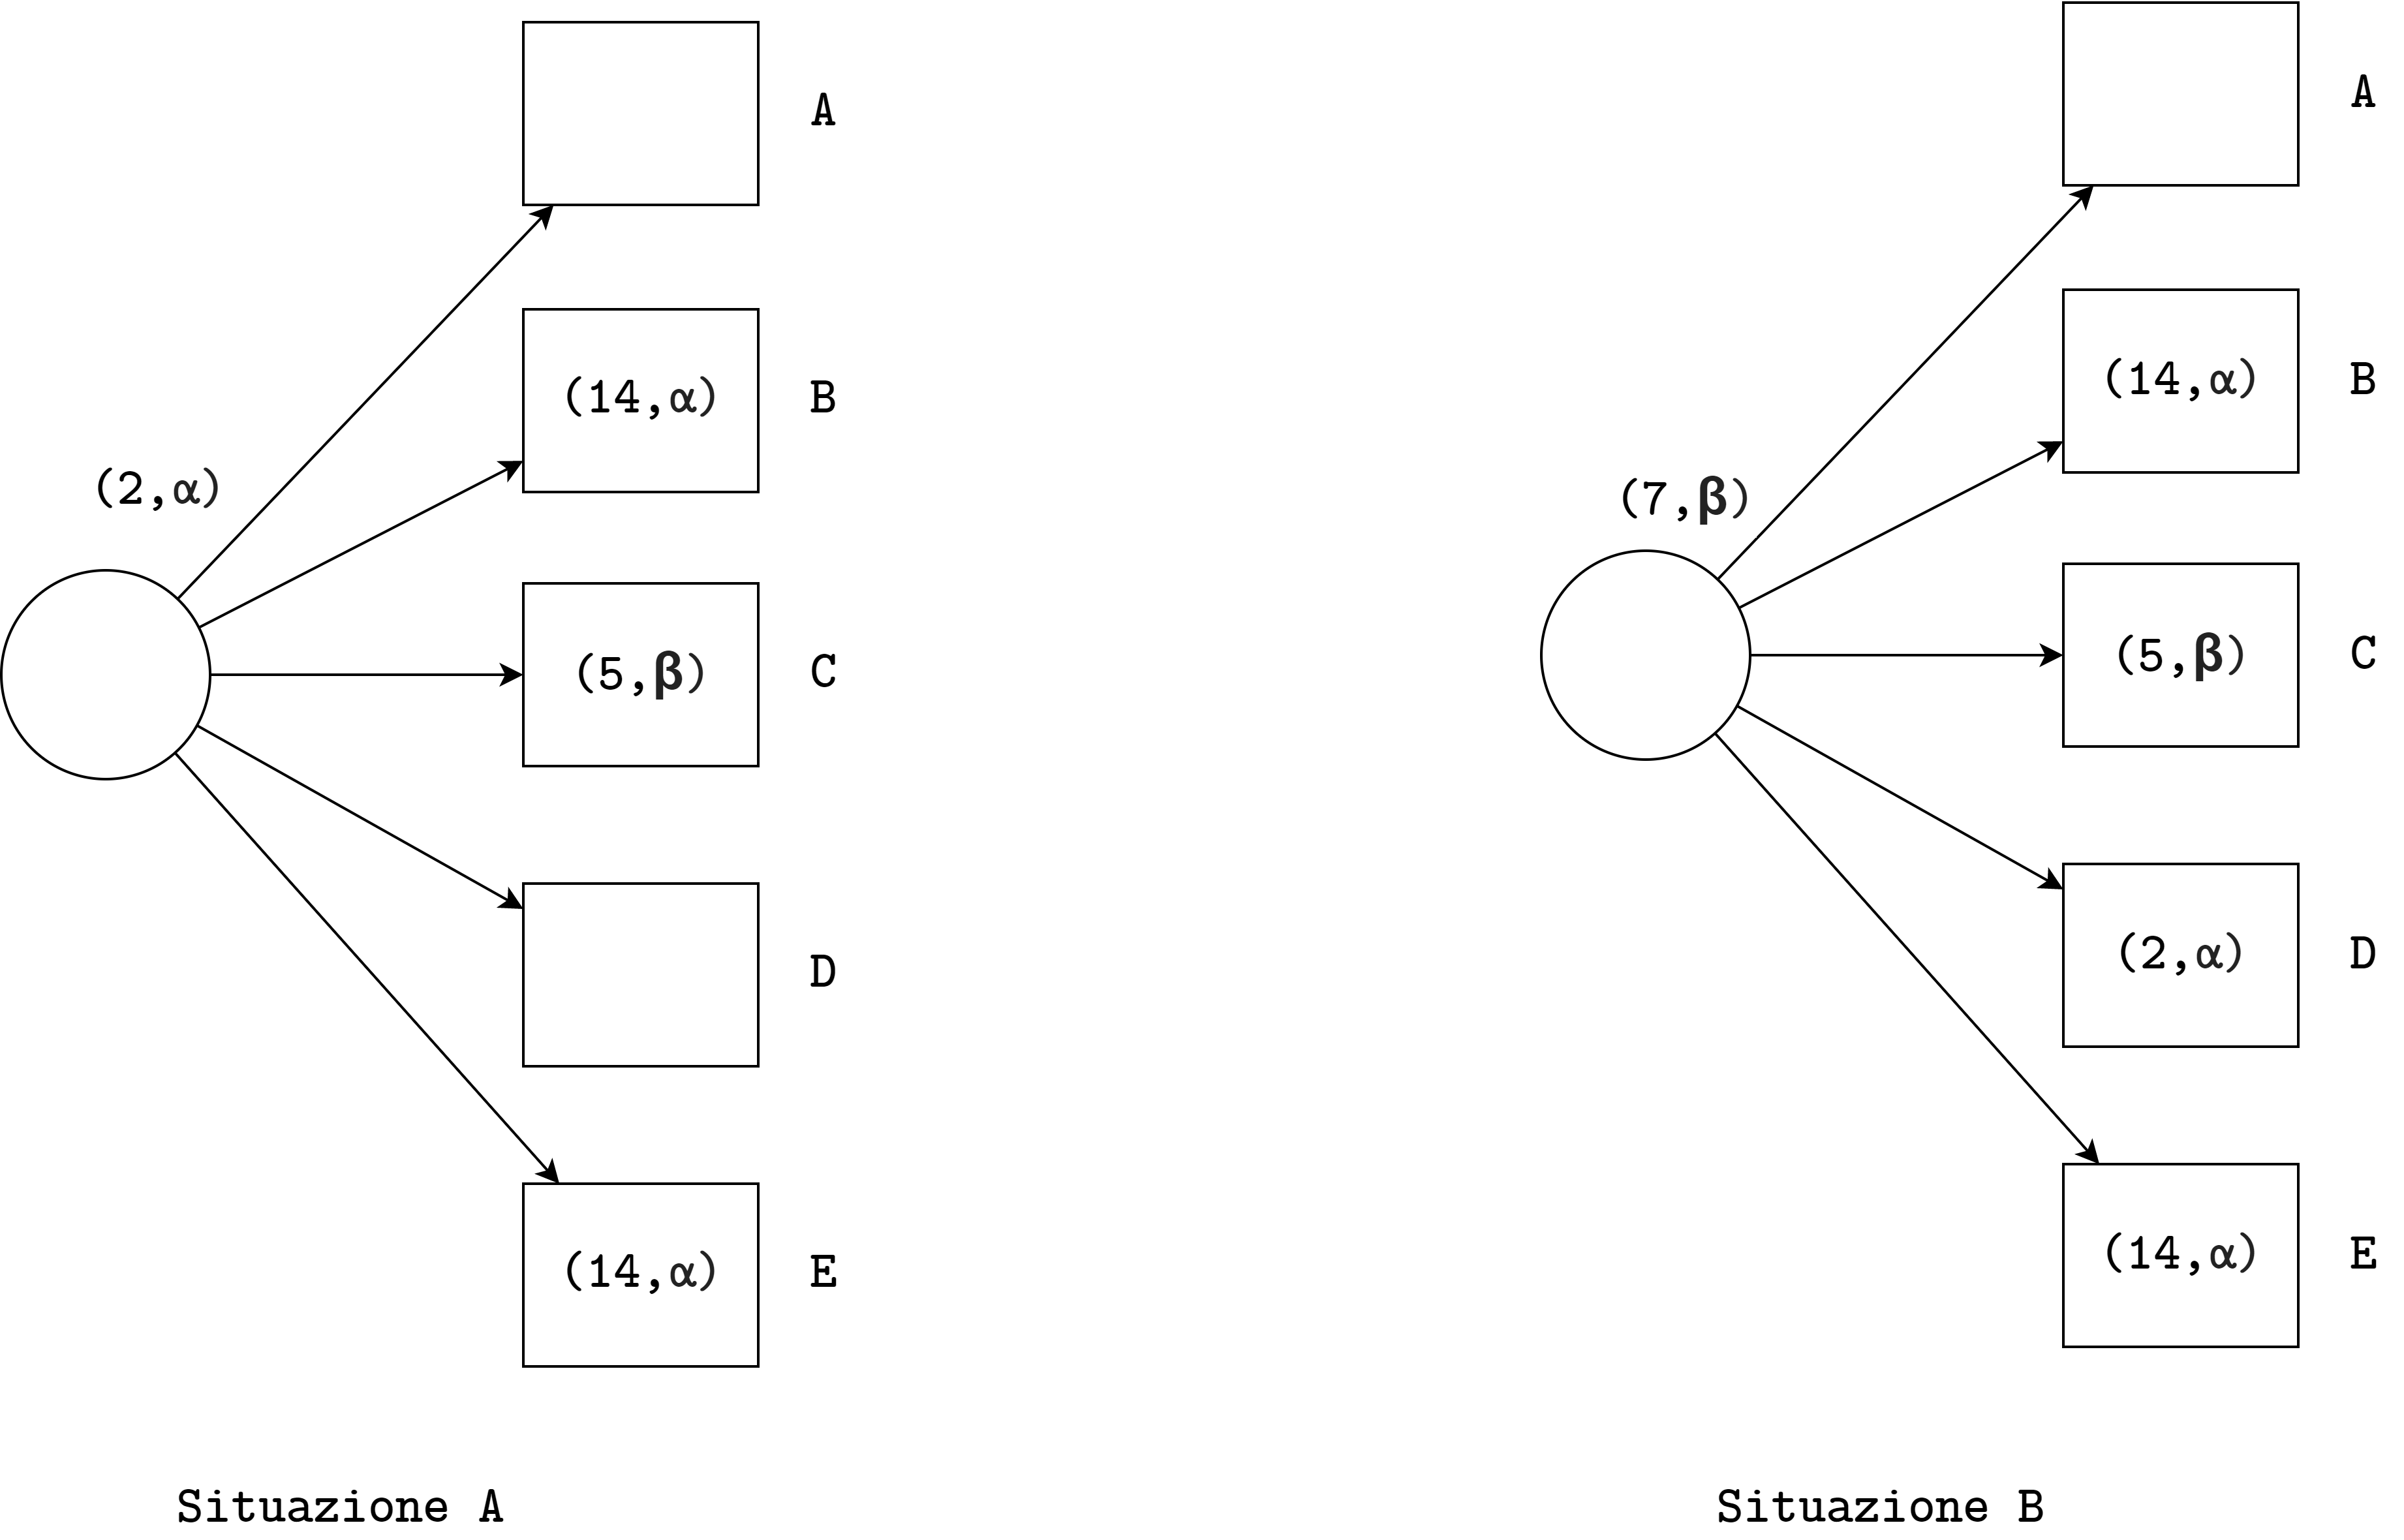
\includegraphics[width=6cm]{./Images/cap2/2.12.png}
\end{figure}

Esempio: nella situazione A un proposer può proporre qualunque valore purché nessun acceptor in S abbia accettato alcuna proposta con numero seriale minore di 2. Nella situazione B invece il proposer deve proporre $\beta$, cioè il valore associato alla proposta con numero seriale più alto (5) tra quelle accettate con numero minore di 7 (5 e 2).

\subsubsection{GENERAZIONE DELLE PROPOSTE}
Affinché il requisito P2\textsuperscript{c} sia soddisfatto, quando intende effettuare una proposta con numero $n$, un proposer deve conoscere (se esiste) il valore della proposta con numero seriale più alto minore di $n$:
\begin{enumerate}
    \item accettata da ogni acceptor in una maggioranza;
    \item che sarà accettato da ogni acceptor in una maggioranza.
\end{enumerate}
Mentre conoscere le proposte accettate è abbastanza semplice, prevedere le scelte future degli acceptor è piuttosto complicato. A questo proposito il proposer di una proposta con numero $n$ lo può controllare richiedendo agli acceptor la promessa di non accettare ulteriori proposte con numero minore di $n$.

\vspace{5mm}

\begin{itemize}
    \item Per questa richiesta di \texttt{prepare} con numero $n$, il proposer sceglie un numero ed invia una richiesta ad ogni membro di un insieme di acceptors richiedendo la promessa di non accettare mai una richiesta con numero seriale inferiore a $n$ (\textbf{promise}), e il valore della proposta che esso ha già accettato con il più grande numero seriale minore di $n$, se presente.
    \item Per la richiesta di \texttt{accept}, se il proposer riceve da una maggioranza degli acceptors risposta alla richiesta di \texttt{prepare}, invia ad essi una richiesta di \texttt{accept} per una proposta con numero $n$. Il valore $v$ associato alla proposta può essere:
    \begin{itemize}
        \item il valore della proposta con numero seriale più alto tra quelle delle risposte degli acceptors;
        \item un qualsiasi valore, nel caso in cui le risposte non riportavano proposte precedenti.
    \end{itemize}
\end{itemize}
Il funzionamento è spiegato in maniera semplice nelle immagini successive:

\begin{figure}[ht]
    \centering
    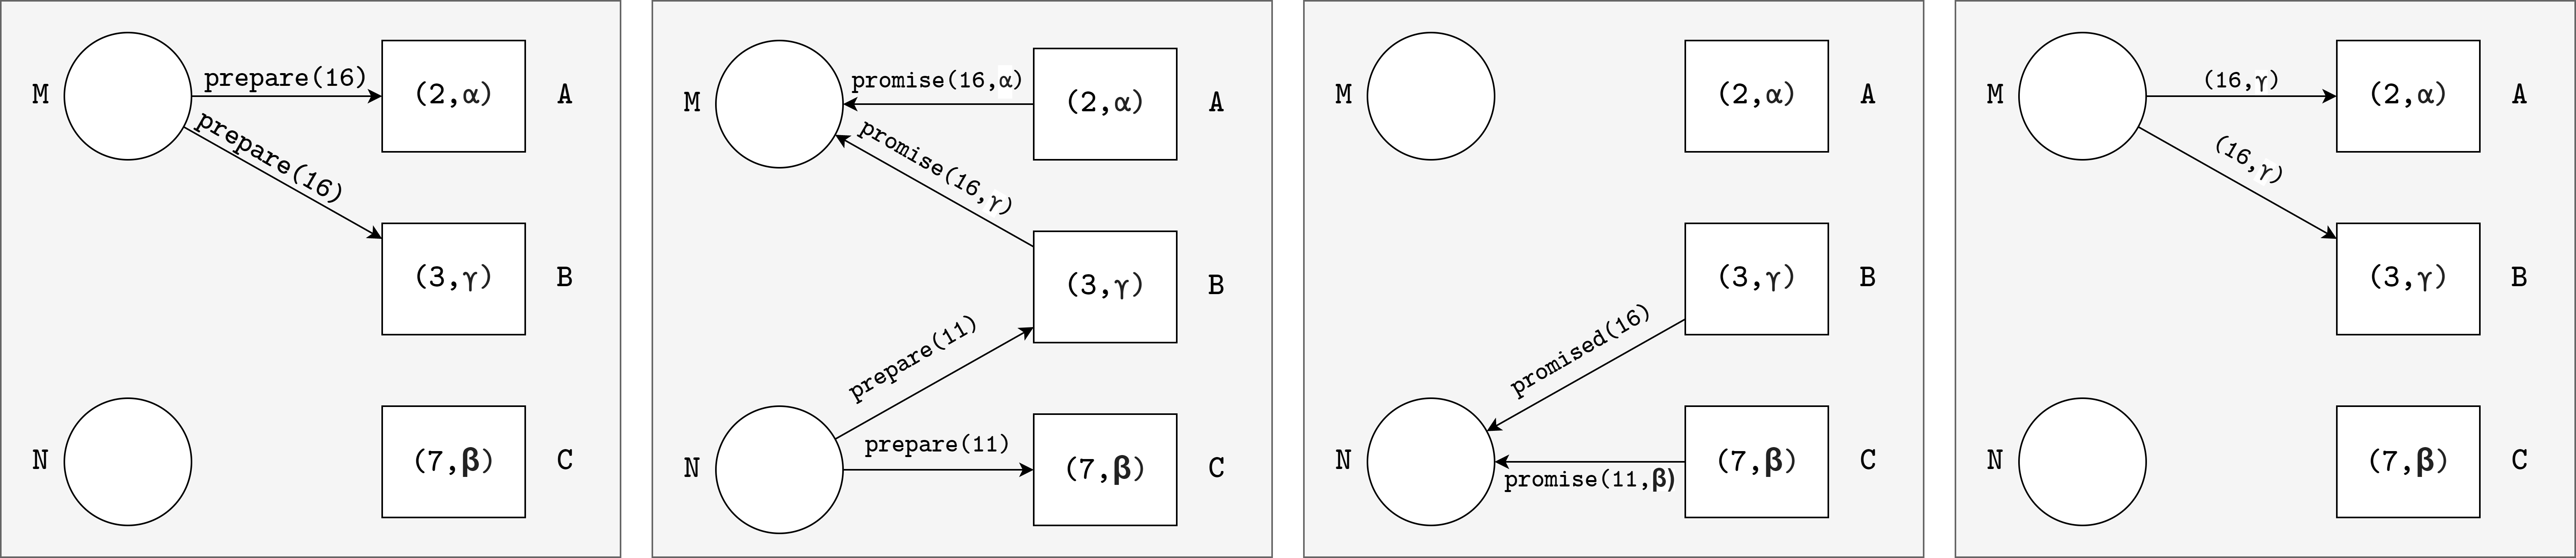
\includegraphics[width=14cm]{./Images/cap2/2.13.png}
\end{figure}

\subsubsection{COMPORTAMENTO DEGLI ACCEPTOR}
\begin{itemize}
    \item Gli acceptor possono ricevere due tipi di messaggi: \texttt{prepare} e \texttt{accept}. 
    \item Un acceptor può sempre rispondere ad una richiesta di tipo \texttt{prepare}.
    \item Un acceptor può rispondere ad una richiesta di tipo \texttt{accept}, accettando la proposta, solo se non ha promesso a qualche processo di non farlo.
\end{itemize}
Viene quindi formulato il seguente requisito:

\noindent\textbf{P1\textsuperscript{a}: Un acceptor può accettare una proposta con numero seriale \textit{n} se e solo se non ha risposto ad una richiesta prepare il cui numero è maggiore di \textit{n}.}

Un acceptor può ignorare una richiesta \texttt{prepare} per la quale non è in grado di effettuare una promessa, ovvero può non rispondere a richieste di tipo \texttt{prepare(m)} dove sia già stato un messaggio \texttt{promise(n)} con $n > m$. Un acceptor può inoltre ignorare richieste \texttt{prepare} relative a proposte già accettate (messaggi duplicati).

\vspace{5mm}

Ogni acceptor è quindi tenuto a mantenere in memoria stabile:
\begin{enumerate}
    \item la proposta di numero seriale più elevato accettata;
    \item il numero seriale della richiesta \texttt{prepare} con numero maggiore a cui ha risposto con un messaggio \texttt{promise}.
\end{enumerate}
In questo modo soddisfa l'invariante P2\textsuperscript{c} anche in seguito al riavvio dopo un fallimento.

Nella formulazione classica gli acceptor sono replicati attivamente, ma è anche possibile una formulazione passiva. Un coordinatore riceve le richieste dai proposers, e rappresenta il frontend del sistema di processi alla base di Paxos, e smista le richieste ai vari acceptors e learners. Il coordinatore propaga anche il valore per cui si è raggiunto il consenso.

\subsubsection{ALGORITMO - FASE 1}
\begin{itemize}
    \item Un proposer selezione un numero di proposta $n$ ed invia una richiesta \texttt{prepare(n)} ad una maggioranza di acceptors.
    \item Quando un acceptor riceve una \texttt{prepare(n)}, se $n$ è maggiore di ogni altra \texttt{prepare} a cui ha già risposto, risponde con una \texttt{promise} di non accettare più proposte con numero seriale minore di $n$ e con il valore della proposta già accettata con numero più grande.
\end{itemize}

\begin{figure}[ht]
    \centering
    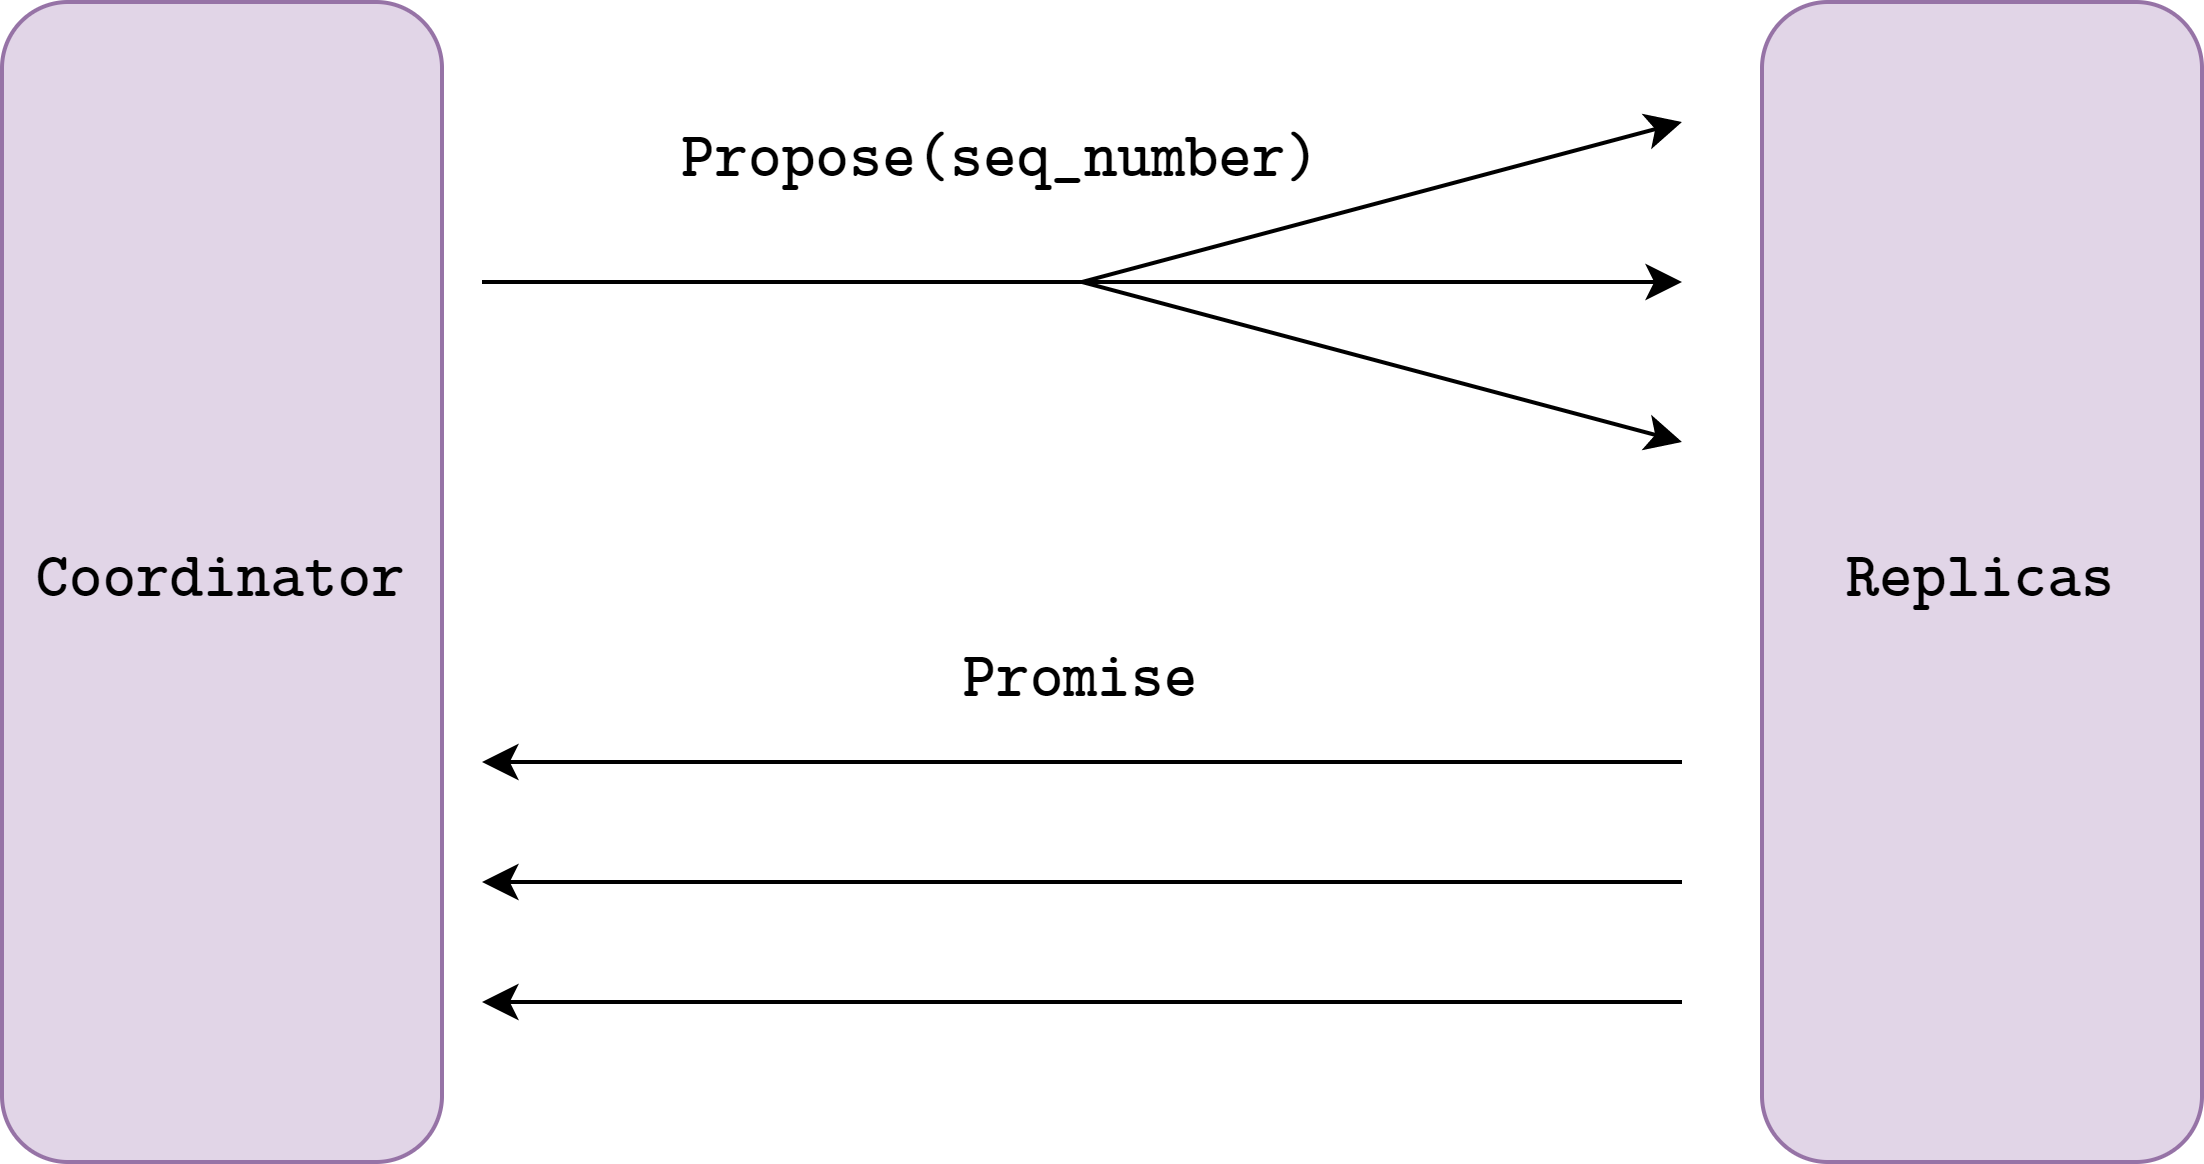
\includegraphics[width=6cm]{./Images/cap2/2.14.png}
\end{figure}

\subsubsection{ALGORITMO - FASE 2}
\begin{itemize}
    \item Se il proposer riceve un messaggio \texttt{promise(n,v)} da una maggioranza degli acceptors, invia un messaggio \texttt{accept(n,v)} a tali acceptors, dove $v$ è il valore della proposta con numero seriale più alto tra quelle riportate dagli acceptors, ovvero un qualsiasi valore, nel caso in cui le risposte non riportavano di una proposta precedente.
    \item Se un acceptor riceve un messaggio \texttt{accept(n,v)}, accetta la proposta a meno che non abbia già risposto ad una richiesta \texttt{prepare} avente numero seriale maggiore di $n$.
\end{itemize}

\begin{figure}[ht]
    \centering
    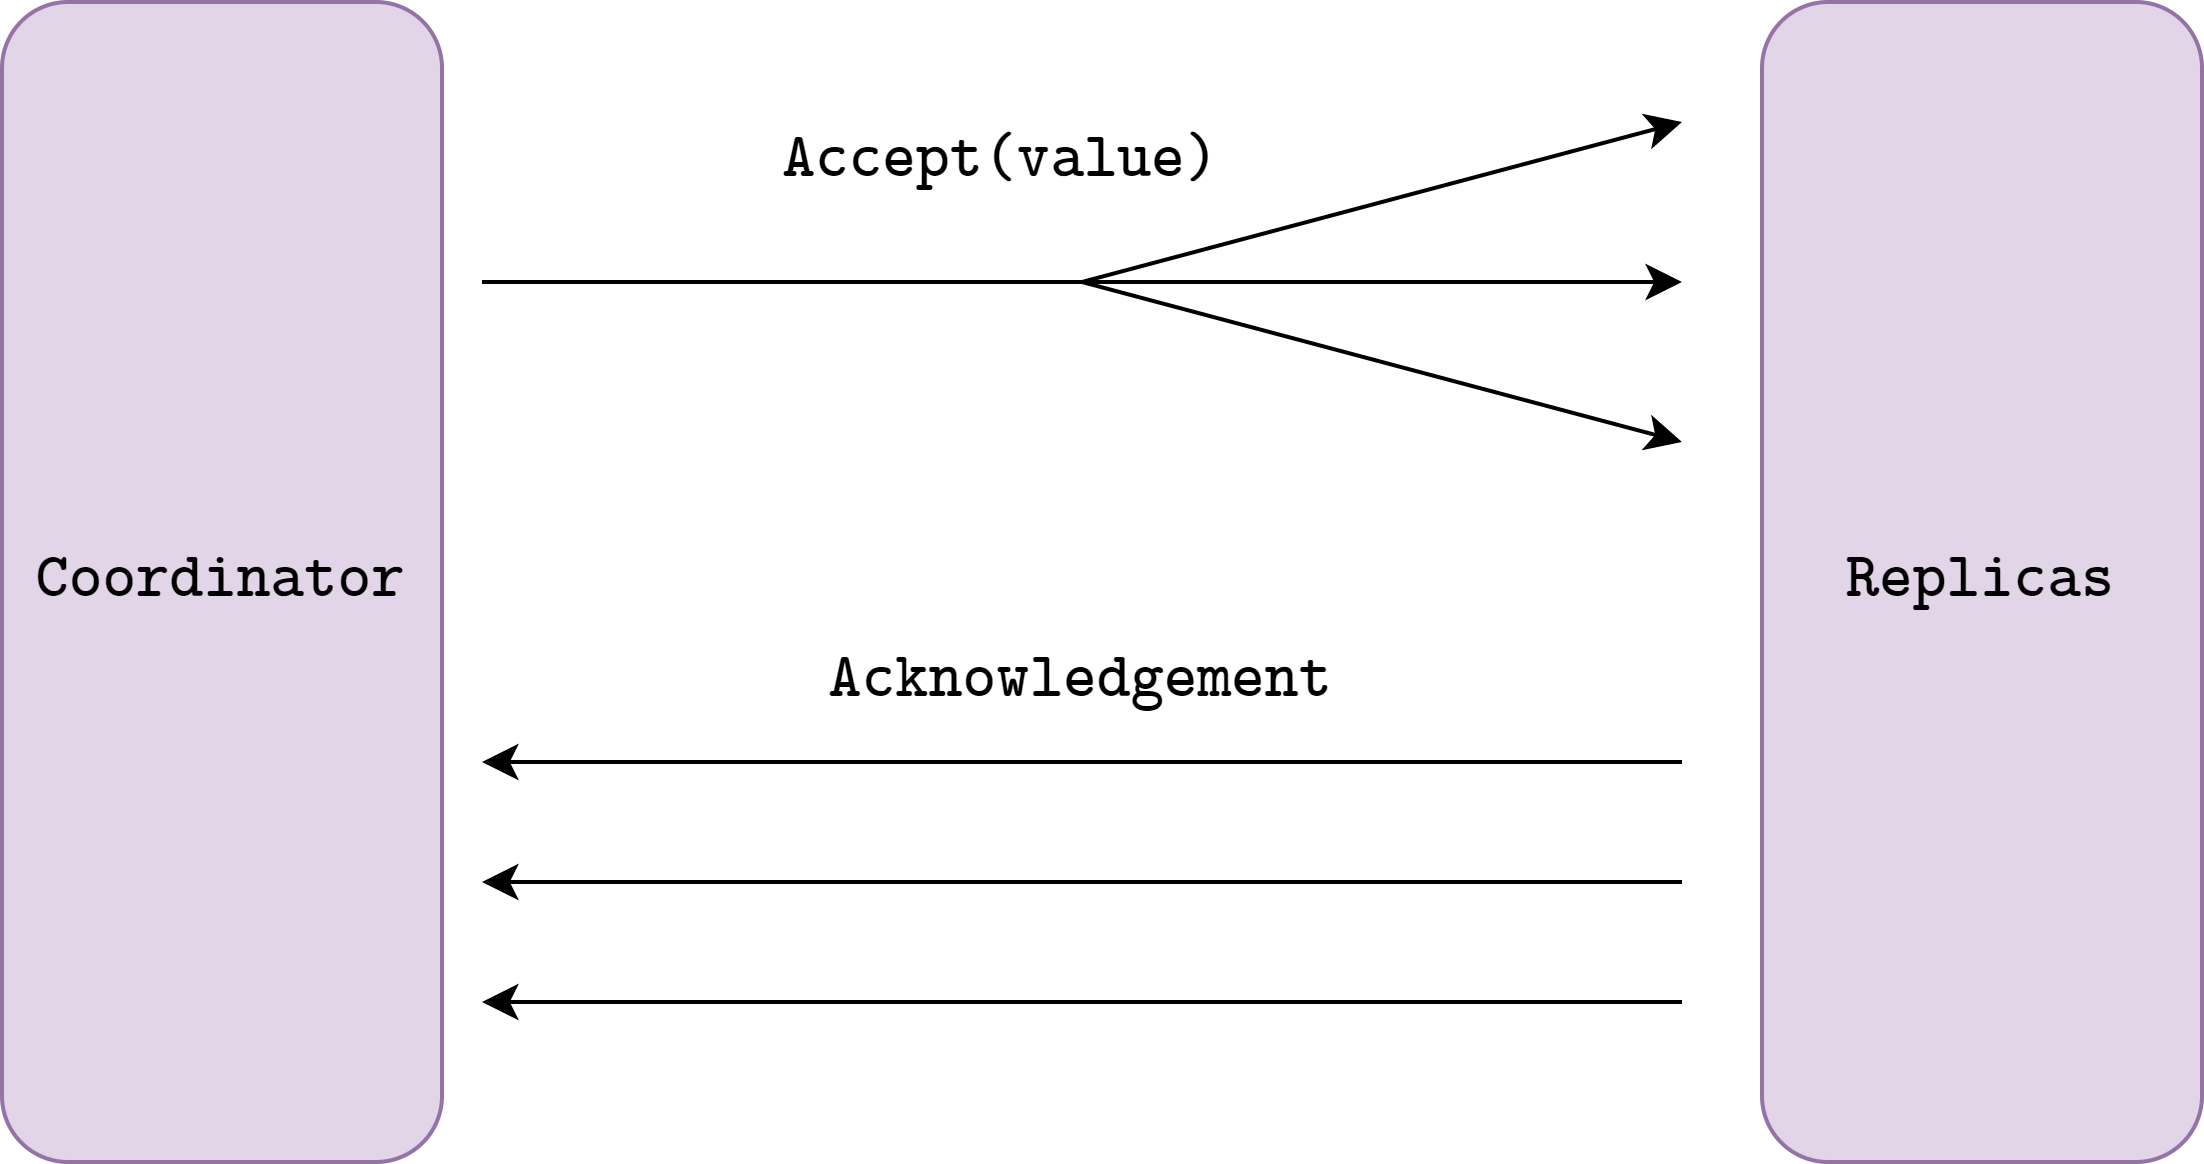
\includegraphics[width=6cm]{./Images/cap2/2.15.png}
\end{figure}
\subsubsection{ALGORITMO - FASE 3}
\begin{itemize}
    \item Se il proposer riceve tanti messaggi di \texttt{ack(n,v)} quanta la maggioranza degli acceptors, allora risponde con un \texttt{commit(n,v)} per comunicare il raggiungimento del consenso.
\end{itemize}

\begin{figure}[ht]
    \centering
    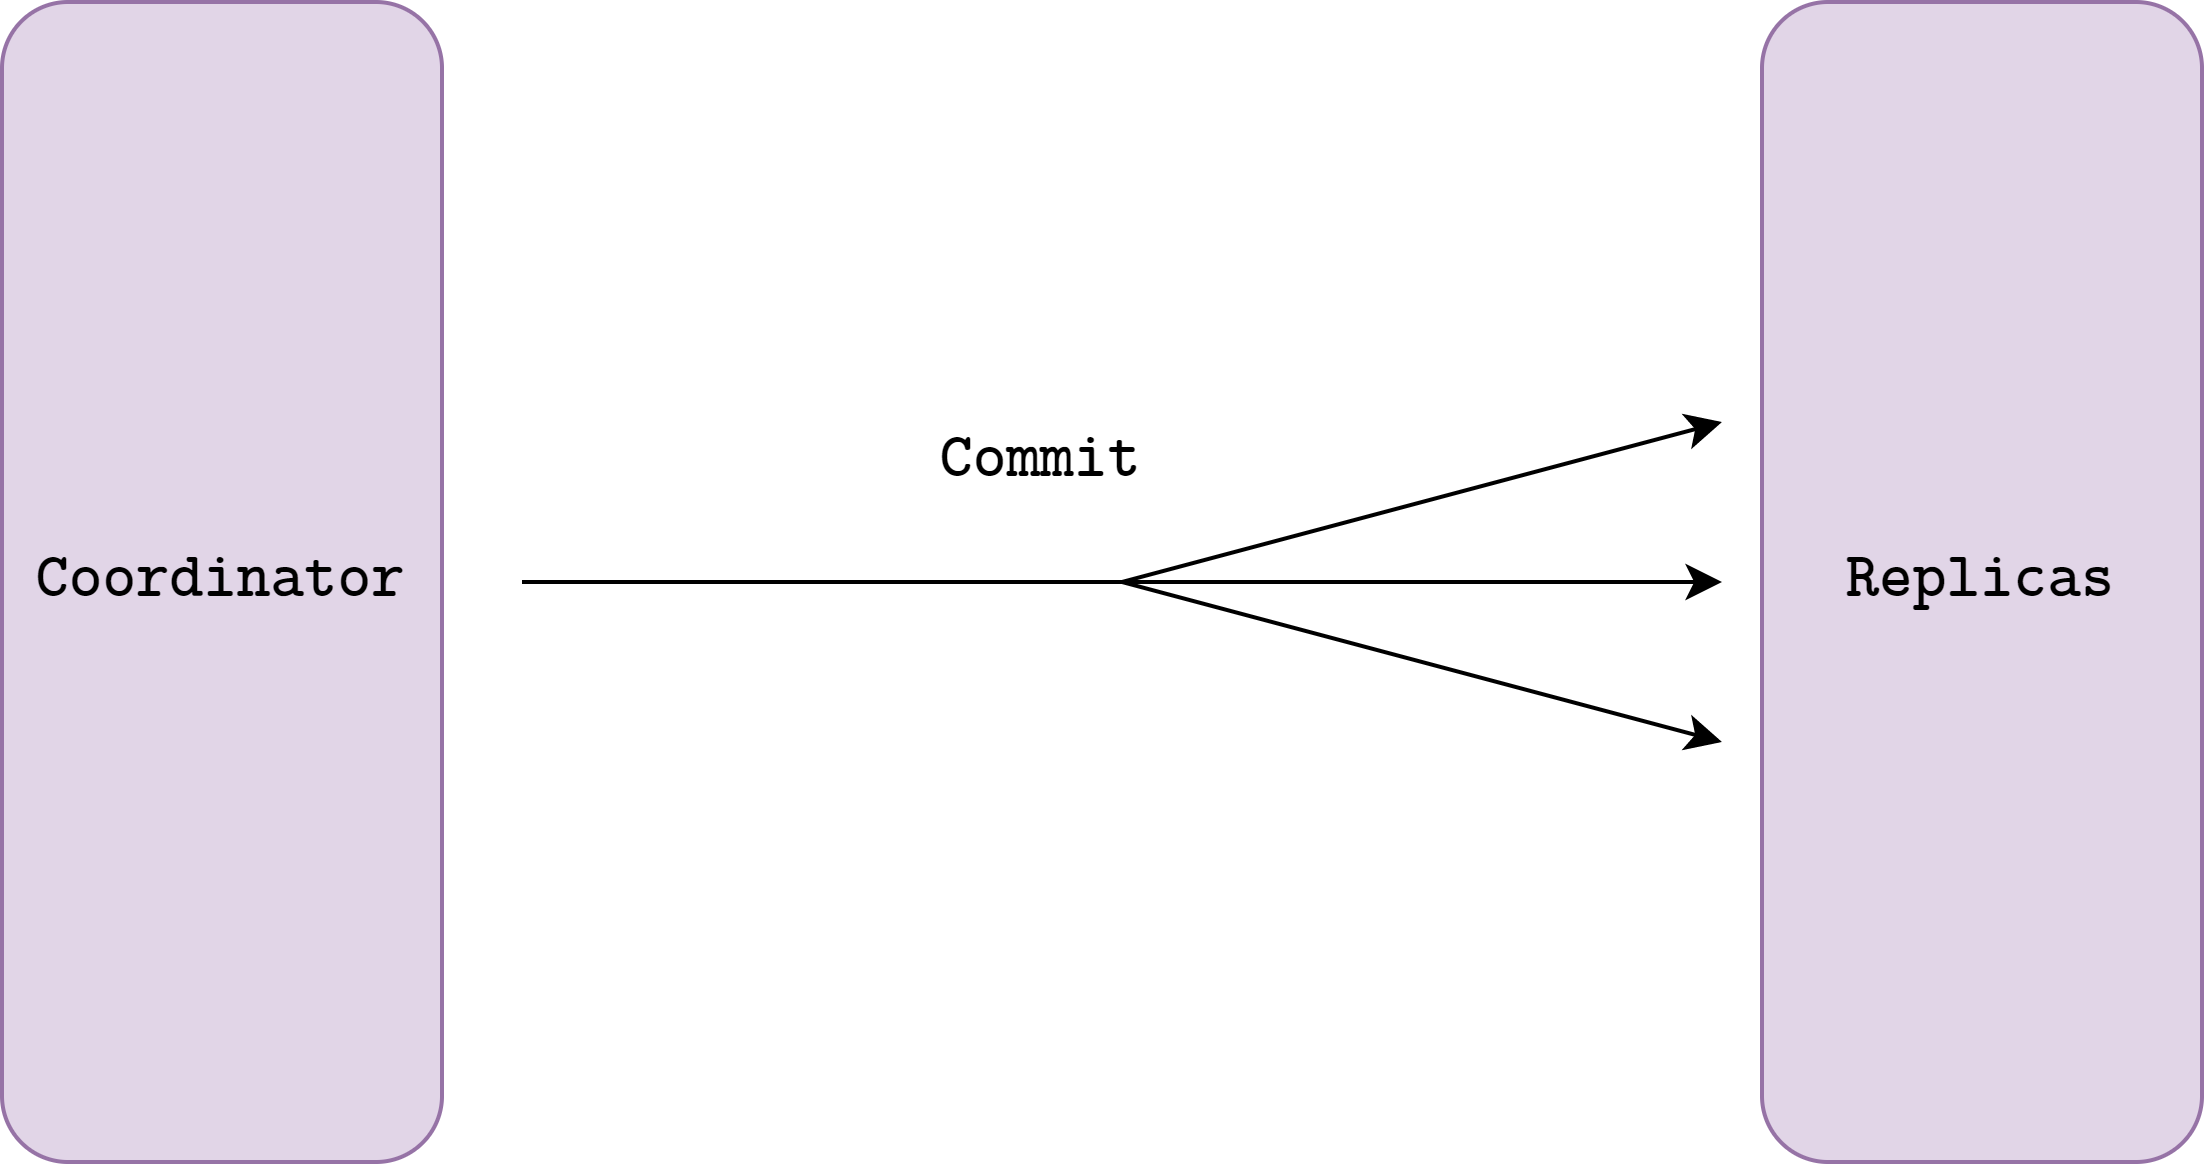
\includegraphics[width=6cm]{./Images/cap2/2.16.png}
\end{figure}
\vspace{5mm}
Si può dimostrare che la fase 2 dell'algoritmo ha il minor costo possibile per un algoritmo di consenso in presenza di fallimenti. In altri termini, Paxos può essere considerato l'ottimo. Per garantire la consistenza dello stato degli acceptors e disaccoppiare dal proposer la fase decisionale sul consenso, entrano in gioco i processi learner. Nelle figure è mostrato un esempio delle tre scelte disponibili:
\begin{figure}[ht]
    \centering
    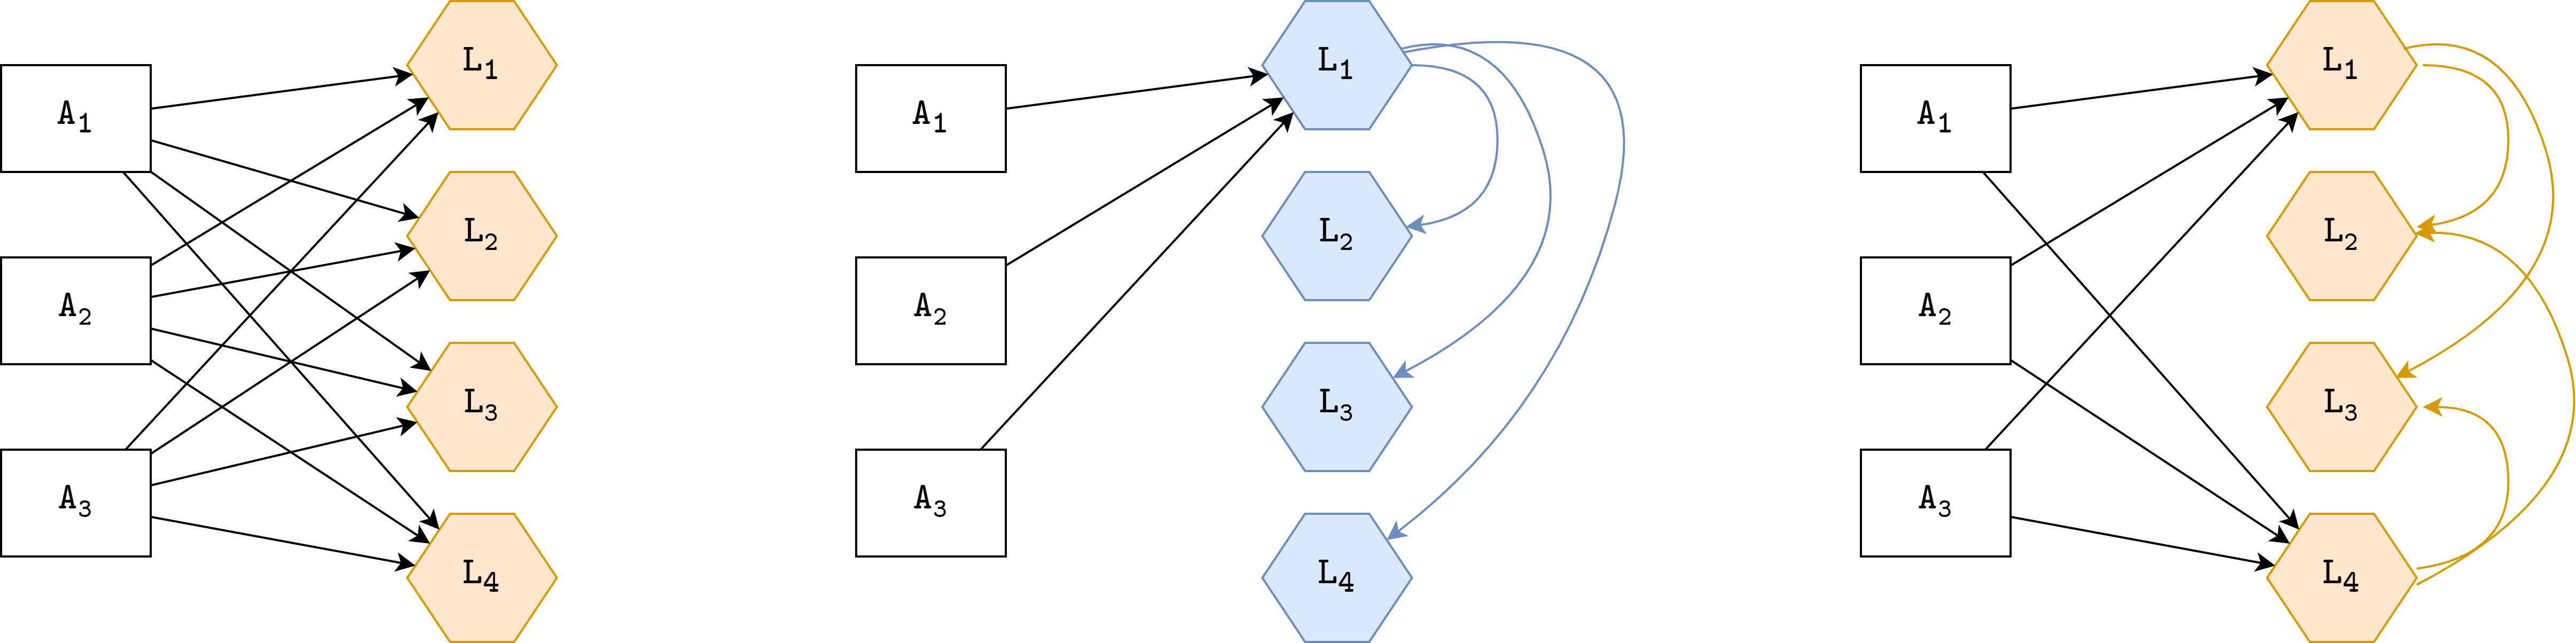
\includegraphics[width=12cm]{./Images/cap2/2.17.png}
\end{figure}

\begin{itemize}
    \item Ogni acceptor informa tutti i learner circa l'accettazione di un valore.
    \begin{itemize}
        \item $\sharp msg = N_{A} \cdot N_{L}$
        \item Tollera il crash di $N_{L}-1$ learner.
    \end{itemize}
    \item Gli acceptor informano un solo learner distinto, che poi informa tutti gli altri learner.
    \begin{itemize}
        \item $\sharp msg = N_{A} + N_{L}-1$
        \item In caso di crash del learner distinto il valore scelto viene perso.
    \end{itemize}
    \item Gli acceptor informano un sottoinsieme di learner che poi provvedono ad informare gli altri learner.
    \begin{itemize}
        \item $\sharp msg = N_{A} \cdot N'_{L} + N'_{L} \cdot (N_{L} - N'_{L})$
        \item Tollera il crash di $N'_{L}-1$ learner.
    \end{itemize}
\end{itemize}
\subsubsection{PROGRESSO}
Il progresso non è garantito:
\begin{itemize}
    \item Il proposer p completa la fase 1 con una proposta con numero $n_{1}$.
    \item Un altro proposer q completa la fase in con una proposta con numero $n_{2} > n_{1}$.
    \item Durante la fase 2, le \texttt{accept} di p sono ignorate poiché gli acceptor hanno promesso di non accettare proposte con numero minore di $n_{2}$.
    \item Quindi p ricomincia la fase 1 con una proposta con numero $n_{3} > n_{2}$.
    \item Le \texttt{accept} inviate da q con numero $n_{2}$ saranno ignorate (gli acceptor nel frattempo hanno fatto promessa a p di non accettare proposte con numero minore di $n_{3}$).
    \item q fa una proposta con numero $n_{4} > n_{3}$...
\end{itemize}
Per garantire la \textit{liveness} si può eleggere un proposer distinto, che deve essere l'unico processo autorizzato ad effettuare proposte (e quindi ad inviare i messaggi di \texttt{prepare}). Se non si verifica un numero eccessivo di guasti nelle restanti componenti del sistema (proposers, acceptors e rete di comunicazione), è possibile raggiungere il consenso con un singolo proposer. 

Del resto sappiamo che \textbf{non esiste alcun algoritmo deterministico in grado di garantire il raggiungimento del consenso in un sistema asincrono a scambio di messaggi anche nel caso di un unico fallimento per crash di un processo}, per cui occorre un algoritmo per l'elezione del proposer distinto, il quale richiede l'introduzione di casualità o timeouts. La liveness è pertanto garantita esclusivamente durante i periodi di sincronia del sistema. La \textit{safety} invece è garantita a prescindere dalla sincronia.

\subsubsection{FAST PAXOS}
Una versione di Paxos nella quale un proposer p che ha un valore da proporre invia il valore al coordinatore \textit{c} con un messaggio di \texttt{propose}. Il coordinatore quindi invia l'apposito messaggio \texttt{accept} agli acceptor, che sarà seguito dal messaggio \texttt{learn} ai learner. Il ritardo tra la proposta e l'apprendimento è di 3 messaggi.

Fast Paxos si basa sull'idea di risparmiare un messaggio e ridurre il ritardo tra la proposta e l'apprendimento consentendo al proponente di inviare il proprio valore direttamente agli accettori. Ciò però implica la necessità di un quorum più ampio.

\subsection{Consenso sicuro}
La maggior parte dei lavori esistenti riguardanti il consenso sono stabiliti sotto il presupposto che la rete e tutti i nodi siano sicuri. Potrebbe verificarsi un attacco di manipolazione dei messaggi nella rete, dove il nodo attaccante potrebbe essere un nuovo partecipante alla rete o un nodo compromesso che era precedentemente un nodo sicuro.

Lo stato del nodo di attacco è selezionato arbitrariamente, e possono esserci principalmente due tipi di attacchi di manipolazione dei messaggi, ovvero attacco a iniezione costante e attacco a iniezione casuale. Senza alcun meccanismo di difesa, i nodi non possono distinguere lo stato del nodo sicuro e quello dell'attacco in modo che può utilizzare le informazioni del nodo di attacco per aggiornare i propri stati. Attaccanti interni che dispongono di tutti i dati di supporto al consenso, attaccanti esterni che possono riprodurre messaggi autentici, camuffare altri nodi con le loro identità catturate. Gli esterni possono essere facilmente rimossi dall'autenticazione.

\vspace{5mm}

L'effetto degli attacchi sugli algoritmi di consenso:
\begin{itemize}
    \item può far divergere la rete;
    \item può invertire lo stato corretto del sistema/fenomeni osservati;
    \item può far convergere la rete al suo valore iniettato;
    \item Può impedire alla rete di raggiungere un consenso.
\end{itemize}
Una soluzione è calcolare la devianza di ogni nodo dal valore di consenso della maggioranza, e definire affidabili i nodi con una minima deviazione.

Un miglioramento consiste nell'aggiungere la tecnica di autenticazione utilizzando la crittografia basata sull'identità. Supponiamo che un nodo voglia inviare un valore agli altri durante un algoritmo di consenso: esso firma il messaggio con la sua chiave private e lo cifra utilizzando l'identificativo di uno dei possibili destinatari, e quindi lo invia. Il ricevente decifra il messaggio ricevuto utilizzando la sua chiave privata e quindi utilizzando la chiave pubblica del mittente ne verifica la firma, di conseguenza l'autenticità. Se la verifica ha esito positivo, il messaggio può entrare nella procedura di aggiornamento del consenso.


\section{Primitive di comunicazione di gruppo}
Esistono diverse primitive di comunicazione. Prima di tutto distinguiamo il \textbf{gruppo chiuso}, nel quale solo i membri possono inviare messaggi in multicast al gruppo, e \textbf{gruppo aperto}, nel quale anche i non membri possono inviare messaggi in multicast al gruppo. L'obiettivo è assicurarsi che i processi possano scambiare messaggi di gruppo anche in presenza di fallimenti dei canali di comunicazione e/o dei processi stessi.

\vspace{5mm}

Le principali strategie per la consegna affidabile dei messaggi sono:
\begin{itemize}
    \item Error masking: ridondanza spaziale e temporale;
    \item Error detection and recovery: basata su ack e timeout;
\end{itemize}
Ridondanza temporale indica che il messaggio viene inviato più volte: per mascherare $k$ omissioni, il messaggio deve essere inviato $k+1$ volte. In entrambi i casi si pone il problema dei messaggi duplicati, che devono essere scartati dal ricevente. È difficile in generale trovare il giusto compromesso tra semplicità di recovery e consumo di banda.
\subsection{Schemi per ack dei messaggi}
Nello schema con \textbf{positive ack}, un messaggio viene ritrasmesso se non viene ricevuta una conferma al mittente entro un timeout predefinito. La failure viene individuata più rapidamente in un caso di traffico sporadico.

\vspace{5mm}
Nello schema con \textbf{negative ack}, il ricevente richiede una ritrasmissione inviando un ack negativo: minimizza il traffico di rete ma richiede l'implementazione di uno dei seguenti meccanismi:
\begin{itemize}
    \item numerazione dei messaggi, in modo tale da poter richiedere la ritrasmissione di un particolare messaggio:
    \item una strategia \textit{time-triggered} in maniera tale che il ricevente sappia quando deve ricevere un messaggio.
\end{itemize}
\subsection{Multicast}
Nelle comunicazioni multicast si individuano tre livelli di affidabilità:
\begin{itemize}
    \item \textbf{Unreliable multicast} - nessuno sforzo per superare failures dei canali di comunicazione; il multicast è affidabile se lo sono i canali e il mittente.
    \item \textbf{Best-effort multicast} - il mittente compie qualche azione per assicurare la consegna del messaggio, come ad esempio ritrasmettere lo stesso, ma non ci sono garanzie.
    \item \textbf{Reliable multicast} - i partecipanti membri del gruppo si coordinano per garantire che il messaggio venga consegnato a tutti i destinatari corretti.
\end{itemize}
È importante specificare che se la rete è affidabile vuol dire che la primitiva di comunicazione è affidabile, e non la rete stessa, che per definizione non è affidabile (vedi cali di tensione e perdite di connessione).
\subsubsection{BASIC MULTICAST}
Basato su due primitive: B-multicast e B-deliver. Garantiscono che un processo corretto prima o poi riceverà il messaggio, a patto che il mittente non fallisca. La primitiva di B-multicast può essere implementata utilizzando una primitiva per la comunicazione punto-punto su canale affidabile:
\begin{itemize}
    \item \texttt{Bmulticast(g,m): for each process p $\in$ g send(p,m)}
    \item \texttt{Breceive(m) at p: Bdeliver(m) at p}
\end{itemize}
Il Basic Multicast offre del problema dell'ack implosion, spreca larghezza di banda e comunque il mittente può fallire in ogni istante durante l'esecuzione del B-multicast.
\subsubsection{RELIABLE MULTICAST}
Il Reliable Multicast invece (Hadzilacos e Toueg, 1994/ Chandra e Toueg, 1996) soddisfa le seguenti proprietà:
\begin{itemize}
    \item \textbf{Integrity} - un processo correttp $p$ riceme $m$ al più una volta. Inoltre, $p \in group(m)$ e $m$ è stato inviato via multicast da $sender(m)$.
    \item \textbf{Validity} - se un processo corretto $p$ invia $m$ in multicast, prima o poi riceverà $m$.
    \item \textbf{Agreement} - se un processo corretto riceve $m$, allora tutti i processi corretti in $group(m)$ prima o poi riceveranno m. 
\end{itemize}    
Le definizioni delle proprietà del reliable multicast fanno riferimento a processi corretti (cioè che non falliscono mai). Una proprietà valida a prescindere dal fatto che i processi siano corretti o meno si dice \textbf{uniforme}. In particolare abbiamo la \textbf{uniform agreement}: se un processo (corretto o meno) riceve $m$, allora tutti i processi corretti in $group(m)$ prima o poi riceveranno m. 
Vediamo l'implementazione del R-multicast con B-multicast:
\begin{lstlisting}[mathescape=true]
On initialization
    Received:= {};
For process p to R-multicast message m to group g
    B-multicast(g, m);  // $p \in g$ is included as a destination
Pn B-deliver(m) at process q with g=group(m)
    if (m $\notin$ Received)
    then
        Received:= Received $\cup$ {m};
        if ($q \neq p)$
        then
            B-multicast(g, m);
        R-deliver(m);
\end{lstlisting}
L'implementazione soddisfa le proprietà del reliable multicast:
\begin{itemize}
    \item \textbf{Integrità}: discendere dall'integrità dei canali di comunicazione; 
    \item \textbf{Validità}: è evidente che un processo corretto prima o poi fa il B-deliver a sé stesso;
    \item \textbf{Accordo}: discende dal fatto che ogni processo corretto esegue B-multicast dopo B-deliver. Se dunque un processo corretto non effettua R-deliver, ciò può essere dovuto solo al fatto che non ha fatto B-deliver, che può sussistere solo se nessun altro processo corretto ha fatto il B-deliver: in tal caso nessuno farà R-deliver.
\end{itemize}
Questa implementazione è corretta in un sistema asincrono, ma inefficiente (il messaggio è inviato |g| volte a ciascun processo). Inoltre soddisfa anche la proprietà di \textit{uniform agreement}: se ad esempio un processo non è corretto e va in crash dopo aver effettuato un R-deliver, poiché in precedenza ha sicuramente effettuato B-deliver, quindi tutti i processi corretti riceveranno il mesasggio.

\noindent\textbf{N.B.} Se si invertono le istruzioni \texttt{R-deliver(m)} e \texttt{if (q $\neq$ p then B-multicast(g, m)}, l'implementazione non soddisfa più l'uniform agreement.

 \subsubsection{ORDINAMENTO FIFO}
Se un processo corretto invia in multicast $m$ e poi $m'$, allora ogni processo corretto che riceverà $m'$ avrà già ricevuto $m$. (versione uniforme = idem senza "corretto").
\subsubsection{ORDINAMENTO CAUSALE}
Se \texttt{multicast(g,m)} $\rightarrow$ \texttt{multicast(g,m')} dove $\rightarrow$ è la relazione \textit{happened-before} nell'ambito del gruppo g, allora ogni processo corretto che riceverà $m'$ avrà già ricevuto $m$ (versione uniforme = idem senza "corretto").

L'ordinamento causale implica quello FIFO, poiché gli invii di uno stesso processo sono in relazione HB. Infatti l'ordinamento causale estende quello FIFO con l'ordinamento della ricezione dei messaggi, che pur essendo inviati da processi diversi, sono in relazione di potenziale causalità:
\begin{itemize}
    \item Se un processo $p$ invia in multicast un messaggio $m$ ed un processo $p' \neq p$ riceve $m$ prima di inviare in multicast $m'$, allora nessun processo corretto riceve $m'$ a meno che non abbia già ricevuto $m$.
\end{itemize}
\subsubsection{ORDINAMENTO TOTALE}
Se un processo corretto riceve i messaggi $m$ e poi $m'$, allora ogni altro processo corretto che riceve $m'$ avrà già ricevuto $m$. L'ordinamento totale non implica quello FIFO né quello causale.

\begin{figure}[ht]
    \centering
    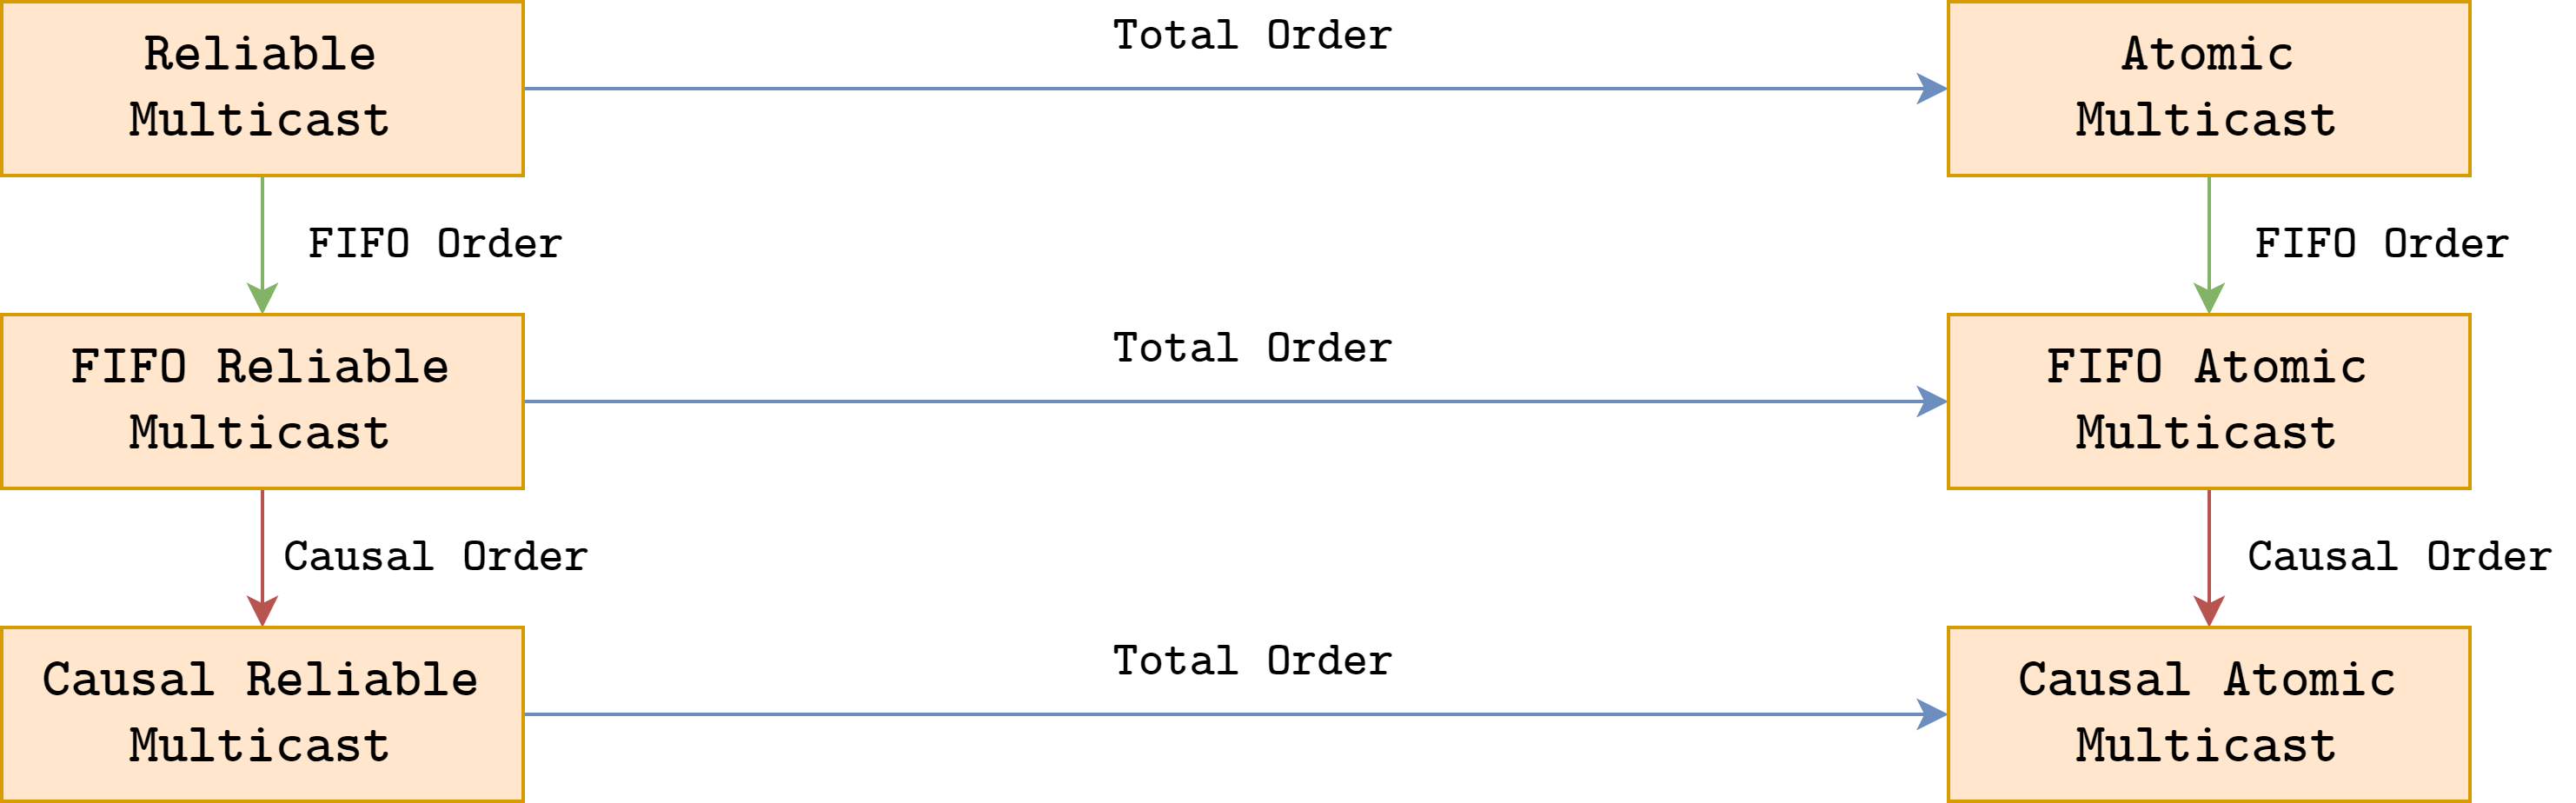
\includegraphics[width=12cm]{./Images/cap2/2.18.png}
\end{figure}

Esempio: una Bulletin Board: c'è un gruppo per argomento; gli utenti si sottoscrivono agli argomenti di interesse. Un utente invia un messaggio su un argomento = broadcast al gruppo. I tipi di semantica che servono sono:
\begin{itemize}
    \item reliable multicast se si vuole garanzia che tutti gli iscritti ricevano i messaggi.
    \item ordinamento FIFO se si vuole che tutti i messaggi inviati da uno stesso utente siano ricevuti nell'ordine di invio.
    \item ordinamento causale se si vuole che il messaggio "Re: info" sia ricevuto dopo il messaggio "info" a cui si riferisce.
    \item ordinamento totale se si vuole che la numerazione dei messaggi sia la stessa per tutti gli utenti.
\end{itemize}

\subsubsection{IP MULTICAST}
La soluzione più comune per realizzare un sistema di comunicazione di gruppo è di impiegare IP multicast, definito al di sopra del protocollo IP, ed un'applicazione può effettuare comunicazioni multicast solo attraverso l'invio di datagrammi UDP.

Un gruppo multicast viene identificato per mezzo di indirizzi di classe D assegnati dalla Internet authority nell'intervallo 224.0.0. - 224.0.0.255. I router sono responsabili dell'opportuna replicazione e instradamento dei pacchetti per la consegna ai membri attraverso il Protocol-Indipendent multicast.

L'IP multicast è un'ottima soluzione per comunicazioni di gruppo in LAN, ma presenta limiti su WAN:
\begin{itemize}
    \item Gli ISP non consentono traffico IP multicast per ridurre il carico sui router e proteggersi da traffico indesiderat;
    \item IP multicasi richiede aggiornamenti all'attuale infrastruttura di rete, che non sono facilmente sostenibili dal business model degli attuali ISP;
    \item IP multicast viola il principio di stateless del protocollo IP, siccome i router devono mantenere informazioni sulla membership dei gruppi;
    \item IP multicast introduce forti complessità e limiti di scala su scenari di ampia scala come internet.
\end{itemize}
Questi motivi hanno portato alla definizione di un nuovo approccio alla comunicazione di gruppo, ovvero Application-Level Multicast.
\subsubsection{APPLICATION-LEVEL MULTICAST}
Una soluzione per ovviare agli inconvenienti di IP multicast è quello di implementare le funzionalità di multicasting a livello applicativo piuttosto che a livello di trasporto della pila ISO/OSI.

Le applicazioni sono interconnesse per mezzo di una overlay network, gestiscono i meccanismi di membership al gruppo e si fanno carico delle operazioni di replicazione e disseminazione dei pacchetti. L'interconnessione al livello overlay può essere strutturata come un albero, oppure non strutturata come una mesh. L'uso di una struttura ad albero implica una maggiore efficienza nella disseminazione, ma anche più vulnerabilità ai fallimenti dei nodi overlay.

L'efficienza ($\eta$) (eta) è misurata come il numero medio di pacchetti scambiati sui link durante la disseminazione di un messaggio in multicast.
\begin{center}
    $\eta_{IPmulticast} = 1$ mentre $\eta_{ALM} < 1$
\end{center}
ALM indica il caso in cui i nodi dell'overlay sono realizzati dagli stessi computer situati presso gli utenti finali. Il risultato è che la distribuzione ottenibile è caratterizzata da una topologia spesso molto lontana dal caso ideale.

Il termine \textbf{Overlay Multicast} è usato per identificare il caso in cui i nodi dell'overlay sono disposti direttamente nella core network, permettendo di realizzare un albero di distribuzione molto più efficiente. A differenza dell'unicast, che deve conoscere tutti i nodi per inviare messaggi, il multicast conosce solo le sorgenti più vicine, in quanto sono i router che si occupano di instradare i pacchetti. Infatti nell'IP multicast viaggia sempre un solo messaggio, mentre nell'ALM sono di meno ma è raro che arrivi al caso peggiore (successione degli unicast).

\subsubsection{ORDINAMENTO FIFO}
L'ordinamento si realizza mediante l'utilizzo di numeri di sequenza. Assumiamo che i gruppi non si sovrappongano:
\begin{itemize}
   \item \texttt{S\textsuperscript{p}} - contatore dei messaggi inviati dal processo \texttt{p} al gruppo \texttt{g}
    \item \texttt{R\textsuperscript{q}} - numero di sequenza dell'ultimo messaggio delivered da \texttt{p}, inviato da \texttt{g} a \texttt{q}.
    \item \texttt{HoldBackQueue(p)} - coda dei messaggi fuori sequenza in attesa di essere ricevuti da \texttt{p}.
\end{itemize}
\begin{lstlisting}[escapeinside={(*}{*)}]
To FO-multicast(m,g):
    (*\texttt{piggyBack(S\textsuperscript{p},m);}*)
    (*\texttt{Bmulticast(m,g);}*)
    (*\texttt{S\textsuperscript{p} = S\textsuperscript{p}+1;}*)
To FO-deliver(q.m) with m bearing S = R\textsuperscript{q}+1:
    (*\texttt{FO-deliver(q,m);}*)
    (*\texttt{R\textsuperscript{q} = S;}*)
To FO-deliver(q,m) with m bearing S > R\textsuperscript{q} + 1:
    (*\texttt{put m in HoldBackQueue();}*)
    (*\texttt{wait until S(m) = R\textsuperscript{q}+1;}*)
    (*\texttt{FOdeliver(q,m);}*)
\end{lstlisting}
\subsubsection{IMPLEMENTAZIONE R-MULTICAST}
Il protocollo multicast affidabile può essere eseguito su UDP e utilizza il servizio multicast IP per la consegna dei pacchetti. Poiché sia IP multicast che UDP sono protocolli inaffidabili, l'affidabilità si ottiene eseguendo un protocollo affidabile end-to-end a livello di applicazione. Per ottenere l'affidabilità, i pacchetti con errori o pacchetti persi verranno ritrasmessi, utilizzando un protocollo a finestra scorrevole basato sul feedback delle stazioni.

Nel costo dell'ALM oltre alla ridondanza temporale realizzata dalle ritrasmissioni, è possibile adottare anche la ridondanza spaziale impiegando percorsi multipli con copie dei messaggi istradati nei vari percorsi, e usando tecniche di codifica per ottenere informazioni addizionali e ricostruire i pacchetti persi dalla rete.

\vspace{5mm}

Application Level Multicast è best effort (se la rete ha delle problematiche si perdono dei messaggi), quindi bisogna aggiungere caratteristiche per aumentare l'affidabilità. Mentre TCP offre garanzie \textit{link by link}, quindi la comunicazione è protetta lungo un canale che collega due endpoint, in questo caso occorre una protezione \textit{end-to-end} perché servono protezioni anche a livello di rete e non solo delle parti, ad esempio se cade un nodo dell'overlay. TCP quindi non va bene per il reliable multicast.

\subsubsection{IMPLEMENTAZIONE ORDINAMENTO CASUALE}
L'implementazione tiene conto solo delle relazioni HB tra i messaggi multicast, non di quelle tra messaggi diretti (one-to-one) scambiati tra i processi. Si può fare però uso di orologi vettoriali (vector clocks), in cui l'elemento i-esimo conta  il numero di messaggi inviati dal processo i-esimo in relazione HB con il prossimo messaggio.

Per effettuare il CO-multicast, un processo incrementa il proprio elemento nel vettore ed esegue B-multicast al gruppo \textit{g} del messaggio marcato con il vector clock. Quando $p_{i}$ fa il B-deliver di un messaggio inviato da $p_{j}$, prima di effettuare il CO-deliver deve inserirlo nella Hold Back Queue finché non ha fatto il CO-deliver di tutti i messaggi in relazione HB con esso. Quindi $p_{i}$ deve verificare di aver fatto:
\begin{itemize}
    \item il CO-deliver di tutti i messaggi precedenti inviati da $p_{j}$;
    \item il CO-deliver di tutti i messaggi da cui $p_{j}$ aveva fatto il CO-deliver prima di inviare il messaggio in questione.
\end{itemize}
Queste condizioni possono essere verificate esaminando i \textit{vector timestamps} dei messaggi ricevuti.

\noindent Il multicast con ordinamento causale affidabile può essere implementato a partire dalla implementazione del Causal Multicast, usando R-multicast al posto di B-multicast.

\subsubsection{IMPLEMENTAZIONE ORDINAMENTO TOTALE}
Basata sulla marcatura dei messaggi con identificatori totalmente ordinati, in modo che tutti i processi possano prendere le stesse decisioni. Il delivery è come per l'ordinamento FIFO, ma i numeri di sequenza si riferiscono al gruppo, non al processo.

Primo metodo: implementazione mediante processo sequenziatore:
\begin{itemize}
    \item un messaggio \texttt{m} è inviato sia a \texttt{g} sia a \texttt{sequencer(g)}, etichettato con un id univoco \texttt{id(m)}
    \item \texttt{sequencer(g)} può coincidere con un membro di \texttt{g}
    \item \texttt{sequencer(g)} gestisce un numero di sequenza per il gruppo \texttt{s\textsubscript{g}}, con cui marca i messaggi di cui effettua B-deliver
    \item \texttt{sequencer(g)} annuncia i numeri di sequenza inviando messaggi di ordinamento a \texttt{g} tarmite B-multicast
    \item un messaggio resta nella Hold Back Queue finché non può esserne effettuato il TO-deliver, in base al suo numero di sequenza.
\end{itemize}
Secondo metodo: algoritmo ISIS (Birman, 1987), valido per gruppi aperti o chiusi. I processi concordano collettivamente sui numeri di sequenza, con un algoritmo distribuito.

Ogni ricevente propone il numero di sequenza al multicaster, che genera il numer \textit{agreed}.
Ogni processo \textit{q} di \textit{g} possiede:
\begin{itemize}
    \item $A^{q}_{g}$: il più alto numero di sequenza finora convenuto;
    \item $P^{q}_{g}$: il più alto numero di sequenza finora proposto dallo stesso \textit{q}.
\end{itemize}
Ogni ricevente propone:
\begin{center}
    $P^{q}_{g}:= max(A^{q}_{g},P^{q}_{g})+1$
\end{center}
e assegna temporaneamente al messaggio il numero proposto, inserendolo nella Hold Back Queue; questa è ordinata con il valore più piccolo in testa.

Il multicaster raccoglie le proposte e seleziona il valore maggiore \textit{a}, quindi effettua \texttt{Bmulticast(i,a)} (\textit{i} è l'id univoco con cui il multicaster ha etichettato \textit{m}).

Ogni ricevente assegna:
\begin{center}
    $A^{q}_{g}:=max(A^{q}_{g},a)$
\end{center}
e associa il valore \textit{a} al messaggio, quindi riordina la Hold Back Queue se il valore convenuto è diverso da quello proposto. Quando al messaggio in testa alla coda viene assegnato il numero \textit{agreed}, viene inserito in una delivery queue.

\subsubsection{IMPLEMENTAZIONE CAUSAL TOTAL MULTICAST}
Se si combina l'algoritmo per l'ordinamento causale (CO) con quello per il multicast totalmente ordinato (TO) basato sul sequencer si ottiene un ordinamento che è ordinato sia causalmente sia totalmente (C\&TO):
\begin{itemize}
    \item il sequenziatore deve fare il delivery secondo l'ordinamento causale, e il multicast dei numeri di sequenza dei messaggi nell'ordine con cui li riceve;
    \item i processi nel gruppo di destinazione non effettuano il deliver prima di aver ricevuto un messaggio order dal sequenziatore e il messaggio è il prossimo nella sequenza;
    \item in tal modo, poiché il sequencer effettua il deliver in ordina causale, e tutti gli altri processi lo effettuano nell'ordine del sequencer, l'ordinamento è sia totale sia causale.
\end{itemize}
Un modo per realizzare un multicast in modo decentralizzato è il \textbf{gossiping}, che alla fine realizza la consegna di messaggi in un overlay costruito con ALM o con reliable multicast.

\subsection{Gossiping}
Il gossiping rappresenta un algoritmo distribuito per poter garantire la consegna di messaggi sebbene fallimenti di link, processo e di rete si possano verificare nel sistema. Realizza una soluzione di flooding selettivo:
\begin{enumerate}
    \item Periodicamente, ogni processo decide di inviare un messaggio a un insieme k di interlocutori scelti in maniera casuale (k è un parametro dell'algoritmo detto fan-out).
    \item Sulla base dei messaggi scambiati, ritrasmissioni vengono attivate.
    \item Messaggi persi vengono recuperati. 
\end{enumerate}
Esistono due modalità di interazione tra i partecipanti a un algoritmo di gossiping:
\begin{itemize}
    \item \textbf{Push style}: il gossiper invia l'informazione a uno o più destinatari scelti casualmente;
    \item \textbf{Pull style}: il gossiper interroga uno o più destinatari richiedendo l'invio di un'informazione.
\end{itemize}
L'informazione che viene scambiata, o \textit{digest}, può essere di due tipi:
\begin{itemize}
    \item \textbf{Positive}: il messaggio di gossiping contiene gli identificativi dei messaggi correttamente ricevuti;
    \item \textbf{Negative}: il messaggio di gossiping contiene gli identificativi dei messaggi noti per essere stati persi.
\end{itemize}
Sono consentite tutte le possibili combinazioni, ma nella pratica nel caso di una strategia di pull si usa un digest negativo, mentre per quella di push uno positivo.

Lo schema pull/negative è intrinsecamente reattivo, mentre quello push/positive è implementato in accordo ad uno schema proattivo. Il gossiping permette di ottenere la consegna affidabile con una data probabilità prossima a 1.

\vspace{5mm}

Uno schema gossiping convenzionale mostra vulnerabilità che possono essere sfruttate in determinati attacchi o per compromettere le applicazioni basate sul gossiping. Spesso sono attacchi di tipo DoS atti a congestionare una porzione di rete o un determinato nodo. Normalmente la scelta dei nodi verso cui inviare messaggi di gossiping è casuale, oppure in base a determinate metriche di qualità.

La protezione contro compromissioni del gossiping è di fondamentale importanza. Gli attacchi Sybil\footnote{\texttt{https://www.sciencedirect.com/topics/computer-science/sybil-attack}} ad esempio vengono evitati usando un servizio di \textbf{Certificate Authority} (CA) che assegna identità ai partecipanti al gossiping in modo che gli avversari malintenzionati non possano falsificare le identità.

Un'altra soluzione è usare primitive crittografiche per proteggere integrità e autenticità dei messaggi scambiati, oppure considerare validi i messaggi di gossiping se ricevuti da un numero elevato di peer.

Un'alternativa è inviare i messaggi di gossiping a porte conosciute pubblicamente mentre si ritrasmettono a porte selezionate casualmente, e scegliendo casualmente i messaggi da scambiare dai digest per evitare di essere sopraffatti da messaggi fasulli.

Il gossiping è utilizzato come sistema di multicast nella blockchain.

\subsection{Failure Detector}
Uno dei problemi che si riscontra nel progetto di un algoritmo distribuito è decidere quando un determinato processo fallisce (con riferimento a fallimenti per crash). Un \textbf{Failure Detector} è un servizio in grado di stabilire se un processo è fallito. Tale servizio è tipicamente implementato da un insieme di oggetti, ciascuno locale ad uno degli \textit{N} processi del sistema distribuito. Ciascun oggetto (detto local failure detector) esegue un algoritmo di detection in congiunzione con le sue controparti eseguite localmente ad altri processi.

\textbf{N.B.} Si assume che i processi falliscano solo per crash, che abbiano canali di comunicazione affidabili, e che il fallimento di un processo non impedisca agli altri di comunicare.

\vspace{5mm}

In un sistema asincrono, il rilevamento di fallimenti è soggetto ad errori poiché un processo può essere considerato come fallito sebbene questo sia correttamente in esecuzione.

La maggior parte dei failure detector sono inaffidabili, restituendo uno dei due risultati sullo stato di fallimento di un processo \textit{q}:
\begin{itemize}
    \item \textbf{Unsuspected}: il detector ha di recente avuto prova che il processo \textit{q} non è fallito (un messaggio è stato ricevuto di recente dal processo; tuttavia ciò non esclude la possibilità che il processo sia fallito da allora).
    \item \textbf{Suspected}: il detector ha indicazioni sul fatto che il processo \textit{q} potrebbe essere fallito (il processo non riceve messaggi per un tempo maggiore del massimo nominale; tuttavia il processo potrebbe funzionare correttamente, ma non rispondere a causa ad esempio di partizionamenti di rete o eccessivi rallentamenti nell'esecuzione).
\end{itemize}
Entrambi i risultati sono da considerarsi suggerimenti: potrebbero non accuratamente riflettere il reale stato del processo \textit{q}.

\vspace{5mm}

Un failure detector affidabile è sempre accurato nel determinare il crash di un processo. Può restituire i risultati:
\begin{itemize}
    \item \textbf{Unsuspected}: come nel caso di detector inaffidabili, rappresenta solo un suggerimento.
    \item \textbf{Failed}: il detector determina con certezza che il processo \textit{q} è fallito. Il processo non eseguirà nessun azione ulteriore (per definizione, un processo fallito per crash permane nel suo stato, senza eseguire altri passi di elaborazione).
\end{itemize}
\subsubsection{FORMALIZZAZIONE}
La formalizzazione dei concetti inerenti i failure detectors è stata fatta da Chandra e Toueg (C\&T).

Siano dati:
\begin{itemize}
    \item Un sistema composto da $n$ processi $Q=\{p_{1}, p_{2}, ..., p_{n}\}$;
    \item Un orologio globale discreto con valori nell'insieme dei numeri naturali, chiamato $\Phi$;
    \item Una funzione \textit{failure pattern} $F: \Phi \rightarrow 2^{Q}$; $F(t)$ indica l'insieme dei processi falliti fino all'istante $t$;
    \item Un'esecuzione infinita $\sigma$ del sistema (run) nell'insieme delle possibili esecuzioni $\Sigma$.
\end{itemize}
Un \textbf{failure detector} $D_{i}$ è un oracolo associato ad un processo $p_{i}$ che monitora gli altri $n-1$ processi e conserva una lista di processi che sospetta essere falliti.

Dunque, è una funzione da $\Phi \times \Sigma$ (tempo e insieme di tutte le esecuzioni) a $2^{Q}$.

$D_{p}(t, \sigma)$ è l'insieme dei processi che il detector di $p$ sospetta siano falliti. Se $q \in D_{p}(t, \sigma)$, diciamo che $p$ sospetta $q$ al tempo $t$ nell'esecuzione $\sigma$.

Se il detector si accorge di aver commesso un errore, può rimuovere dalla lista dei sospetti un processo erroneamente considerato fallito.

\subsubsection{COMPLETEZZA E ACCURATEZZA}

Chandra e Toueg caratterizzano i failure detector in termini di completezza e accuratezza: 
\begin{itemize}
    \item completezza: c'è un istante di tempo dopo il quale ogni processo andato in crash è permanentemente sospettato da un processo corretto.
    \item accuratezza: c'è un istante dopo il quale nessun processo corretto è sospettato da un processo corretto.
\end{itemize}
La completezza indica la capacità del detector di rilevare i fallimenti, evitando che processi falliti siano considerati corretti (falsi negativi)\footnote{Si noti che la completezza da sola non serve a molto: basta considerare tutti i processi come falliti per far piena completezza.}. L'accuratezza indica, invece, la capacità di non rilevare un fallimento in modo errato, cioè di non considerare falliti processi che sono invece corretti (falsi positivi). 

Possiamo distinguere due livelli di completezza...
\begin{itemize}
    \item \textbf{Completezza forte}: prima o poi ogni processo fallito è permanentemente sospettato da \textit{ogni} processo corretto.
    \item \textbf{Completezza debole}: prima o poi ogni processo fallito è permanentemente sospettato da \textit{qualche} processo corretto.
\end{itemize}
...e quattro livelli di accuratezza: i primi due sono detti di \textit{accuratezza perpetua}, mentre il terzo e il quarto sono più difficili da soddisfare. Si possono rendere i requisiti meno stringenti (e più facili da soddisfare) consentendo a un detector di sospettare di un processo corretto in un qualsiasi istante dell'esecuzione, ma eventualmente deve soddisfare una delle prime due proprietà:
\begin{itemize}
    \item \textbf{Accuratezza forte}: i processi corretti non sono mai sospettati da alcun processo corretto.
    \item \textbf{Accuratezza debole}: c'è almeno un processo corretto che non è mai sospettato da alcun processo corretto.
    \item \textbf{Accuratezza forte eventuale}: c'è un istante di tempo dopo il quale i processi corretti non sono sospettati da alcun processo corretto.
    \item \textbf{Accuratezza debole eventuale}: c'è un istante di tempo dopo il quale almeno un processo corretto non è sospettato da alcun processo corretto.
\end{itemize}
Dai livelli appena introdotti, è possibile fornire otto tipi di failure detector:

\begin{table}[hbt!]
\centering
\begin{tabular}{|c|c|c|c|c|}
\hline
\rowcolor[HTML]{EFEFEF} 
\cellcolor[HTML]{EFEFEF}{\color[HTML]{010066} }                              & \multicolumn{4}{c|}{\cellcolor[HTML]{EFEFEF}{\color[HTML]{3531FF} Accuratezza}}                                                                                                                                                                                     \\ \cline{2-5} 
\rowcolor[HTML]{EFEFEF} 
\multirow{-2}{*}{\cellcolor[HTML]{EFEFEF}{\color[HTML]{010066} Completezza}} & {\color[HTML]{3531FF} Strong}                         & {\color[HTML]{3531FF} Eventually Strong}                                  & {\color[HTML]{3531FF} Weak}                          & {\color[HTML]{3531FF} Eventually Weak}                                   \\ \hline
\cellcolor[HTML]{EFEFEF}{\color[HTML]{010066} Strong}                        & \begin{tabular}[c]{@{}c@{}}Perfect\\ $P$\end{tabular} & \begin{tabular}[c]{@{}c@{}}Eventually Perfect\\ $\diamond P$\end{tabular} & \begin{tabular}[c]{@{}c@{}}Strong\\ $S$\end{tabular} & \begin{tabular}[c]{@{}c@{}}Eventually Strong\\ $\diamond S$\end{tabular} \\ \hline
\cellcolor[HTML]{EFEFEF}{\color[HTML]{010066} Weak}                          & $L$                                                   & $\diamond L$                                                              & \begin{tabular}[c]{@{}c@{}}Weak\\ $W$\end{tabular}   & \begin{tabular}[c]{@{}c@{}}Eventually Weak\\ $\diamond W$\end{tabular}   \\ \hline
\end{tabular}
\end{table}

Relazioni:
\begin{center}
    $P \subseteq L$ \quad \quad $\diamond P \subseteq \diamond L$ \quad \quad $S \subseteq W$ \quad \quad $\diamond S \subseteq \diamond W$
\end{center}
\begin{itemize}
    \item \textbf{Perfect failure detector P}(strongly complete, strongly accurate): tutti i processi falliti prima o poi sono sospettati permanentemente da ogni processo corretto, e tutti i processi corretti non sono mai sospettati da alcun processo corretto. 
    \item \textbf{Eventually perfect failure detector $\diamond $P}(strongly complete, eventually strongly accurate): tutti i processi falliti prima o poi sono sospettati permanentemente da ogni processo corretto, e tutti i processi corretti non sono più sospettati da un instante $t$ in poi da alcun processo corretto. 
    \item \textbf{Strong failure detector S}(strongly complete, weakly accurate): tutti i processi falliti prima o poi sono sospettati permanentemente da ogni processo corretto, e almeno un processo corretto non è mai sospettato da alcun processo corretto. 
    \item \textbf{Eventually strong failure detector $\diamond $S}(strongly complete, eventually weakly accurate): tutti i processi falliti prima o poi sono sospettati permanentemente da ogni processo corretto, e almeno un processo corretto è non più sospettato da un istante $t$ in poi da alcun processo corretto. 
    \item \textbf{Weakly complete, strongly accurate failure detector L}: tutti i processi falliti prima o poi sono sospettati permanentemente da qualche processo corretto, e tutti i processi corretti non sono mai sospettati da alcun processo corretto. 
    \item \textbf{Weakly complete, eventually strongly accurate failure detector $\diamond$L}: tutti i processi falliti prima o poi sono sospettati permanentemente da qualche processo corretto, e tutti i processi corretti sono non più sospettati da un istante $t$ in poi da alcun processo corretto. 
    \item \textbf{Weak failure detector W}(weakly complete, weakly accurate): tutti i processi falliti prima o poi sono sospettati permanentemente da qualche processo corretto, e almeno un processo corretto non è mai sospettato da alcun processo corretto. 
    \item \textbf{Eventually weak failure detector $\diamond$W}(weakly complete, eventually weakly accurate): tutti i processi falliti prima o poi sono sospettati permanentemente da qualche processo corretto, e almeno un processo corretto è non più sospettato da un istante $t$ in poi da alcun processo corretto. 
\end{itemize}

\subsubsection{IMPLEMENTAZIONE}
Se $p_{i}$ è un processo corretto o vivo, deve conoscere se $p_{j}$ è fallito. Ci sono due tipi di realizzazioni: \textbf{Ping-Ack}(proattivo) e \textbf{Heartbeat}(reattivo).

\begin{figure}[ht]
    \centering
    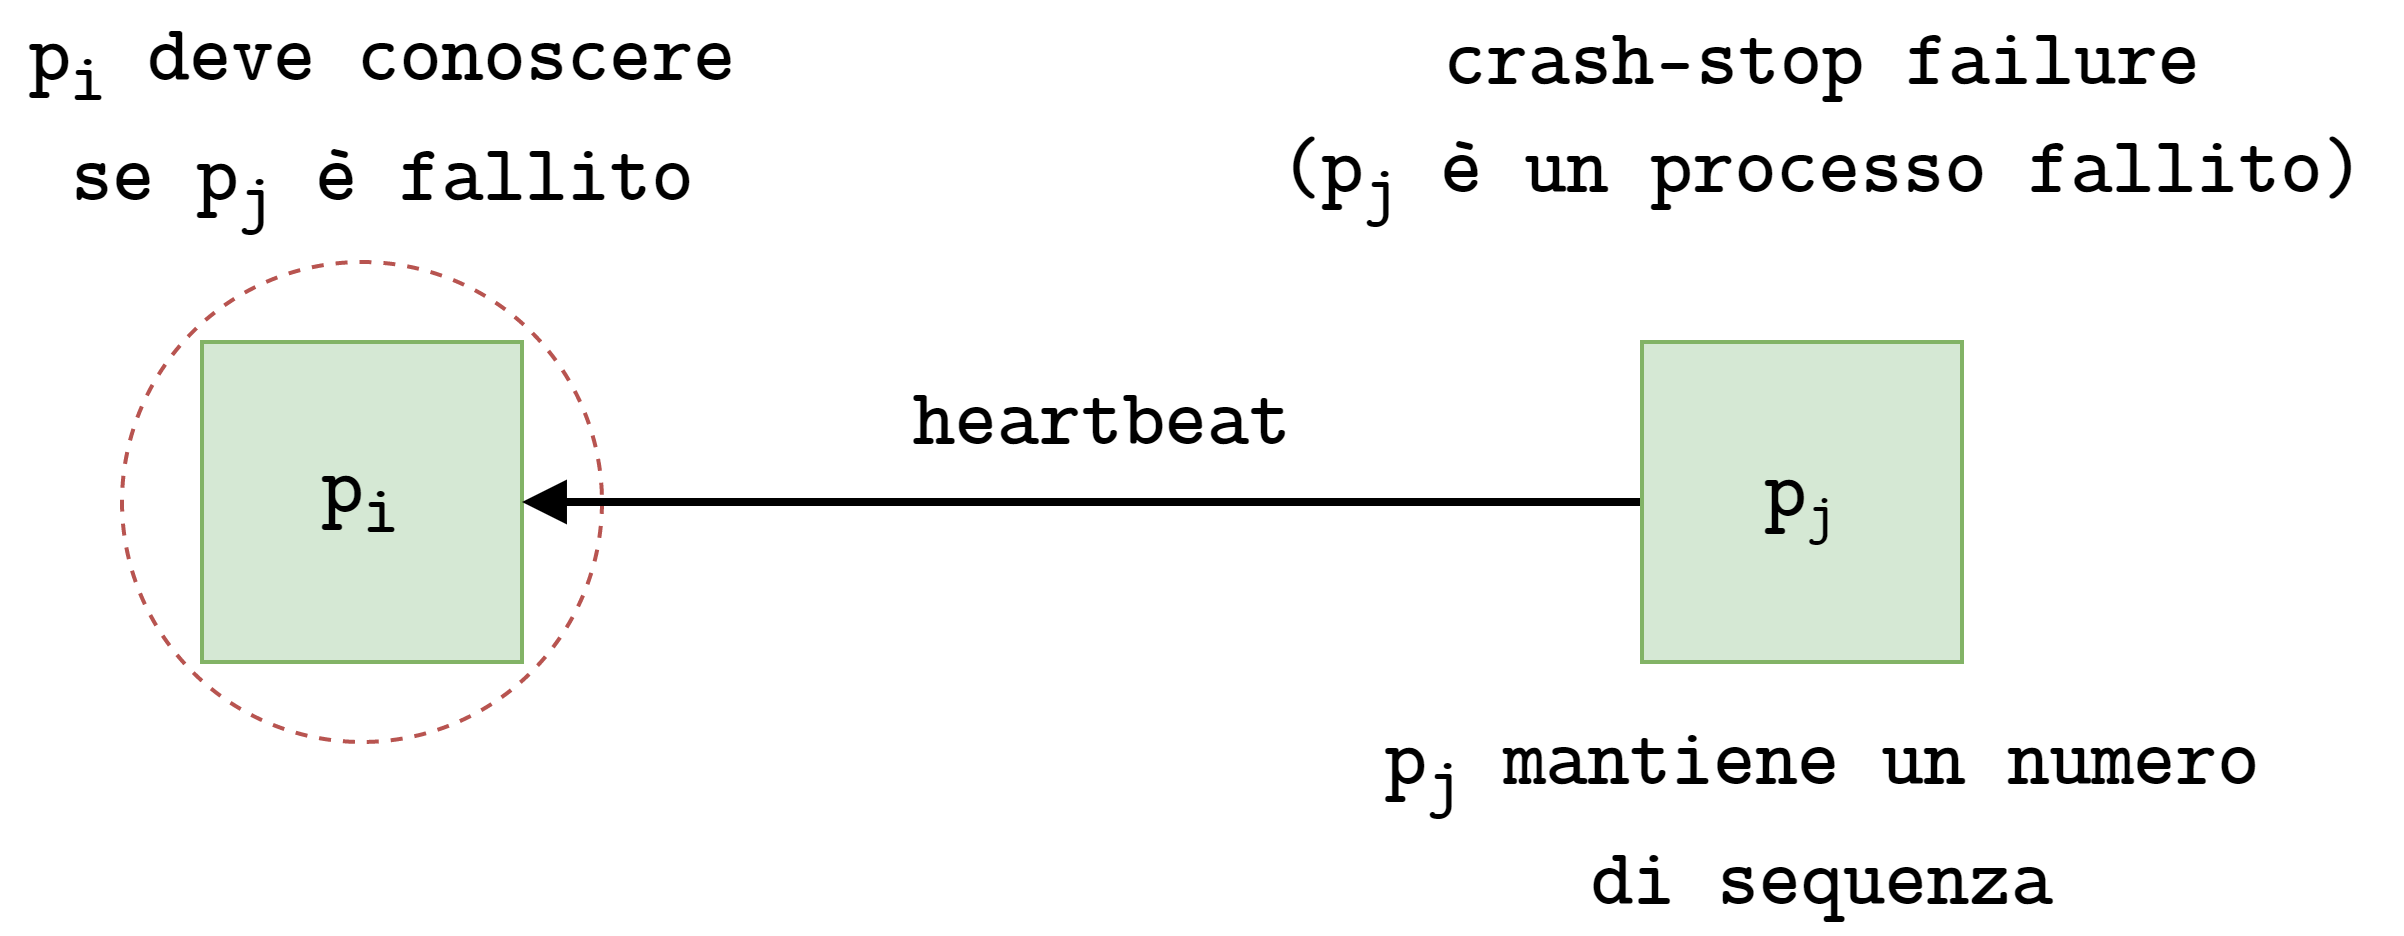
\includegraphics[width=7cm]{./Images/cap2/2.19.png}
\end{figure}

Un failure detector inaffidabile può essere implementato in un sistema asincrono attraverso la tecnica di heartbeat:
\begin{itemize}
    \item Ogni processo p\textsubscript{j} invia un messaggio \textit{"p\textsubscript{j} is alive"} a ciascun altro processo nel sistema distribuito, ogni $T$ secondi.
    \item Il failure detector adotta una stima del massimo tempo di trasmissione di un messaggio, pari a $\Delta$ secondi.
    \item Se il falire detector locale al processo p\textsubscript{i} non riceve un \textit{"p\textsubscript{j} is alive"} entro $T + \Delta$ secondi, allora riporta al processo $q$ che il processo p è \textbf{Suspected}.
    \item Se successivamente riceve un \textit{"p is alive"}, corregge la sua stima, e riporta a $q$ che il processo $p$ è \textbf{Unsuspected}. Altrimenti, assume il processo come fallito.
\end{itemize}
La bontà della risposta fornita ad un processo dipende dall'informazione disponibile localmente. Un failure detector potrebbe dare suggerimenti errati a causa di condizioni di comunicazione estremamente variabili.

Un processo che fallisce per crash inevitabilmente non invierà più messaggi \textit{"p is alive"}; quindi prima o poi ogni altro processo corretto, non ricevendo i messaggi, lo sospetterà di fallimento. Ciò implica \textbf{strong completeness}. Tuttavia, per l'accuratezza possiamo solo pensare che prima o poi i messaggi \textit{"p is alive"} di un processo corretto arriveranno, quindi ci sarà un processo corretto che non sarà sospettato da un altro processo corretto. Ciò implica \textbf{eventual weak accuracy}.

\vspace{5mm}

La scelta dei tempi $T$ e $\Delta$ incide sulle prestazioni del detector. Tempi brevi portano ad indicare spesso come \textit{Suspected} processi che in realtà non sono falliti (falsi positivi), e richiedono molta banda di rete per i messaggi \textit{"p is alive"}. Dall'altra parte, tempi lunghi portano ad indicare spesso come \textit{Unsuspected} processi che in realtà sono falliti (falsi negativi). 

Una soluzione pratica al problema prevede l'uso di valori adattativi per $T$ e $\Delta$, che riflettano le reali condizioni correnti della rete. In questo modo il falire detector resta inaffidabile, ma l'accuratezza aumenta. 

\vspace{5mm}

Un sistema \textbf{parzialmente sincrono} è un sistema inizialmente asincrono ma che dopo un istante (sconosciuto) $t$ diventa sincrono. In questi sistemi, rendendo il timeout adattivo, il detector può essere reso \textbf{eventually perfect} ($\Diamond$P). La \textbf{strong completeness} sussiste per fallimenti di tipo crash. Per la \textbf{eventual strong accuracy}, si osservi che il sistema diventa sincrono da un istante $t$ in poi, dopo il quale si conosce l'intervallo di tempo necessario per inviare un messaggio da $p$ a $q$, per cui prima o poi nessun processo corretto sarà sospettato da un altro processo corretto.

\vspace{5mm}
L'algoritmo di detection diventa affidabile in un sistema sincrono. Infatti $D$ diventa un limite superiore assoluto al ritardo di trasmissione di un messaggio, e non più una stima. L'assenza di un messaggio \textit{"p is alive"} entro $T + \Delta$ permette al failure detector locale di dichiarare con certezza che $p$ è fallito.

È evidentemente che l'algoritmo è molto costoso, vista la richiesta di invio periodico di messaggi di heartbeat. Può essere introdotto un protocollo di detection basato principalmente su messaggi applicativi e che fa uso di messaggi di controllo solo quando il processo che sta monitorando non invia alcun messaggio applicativo al processo monitorato.

\begin{figure}[ht]
    \centering
    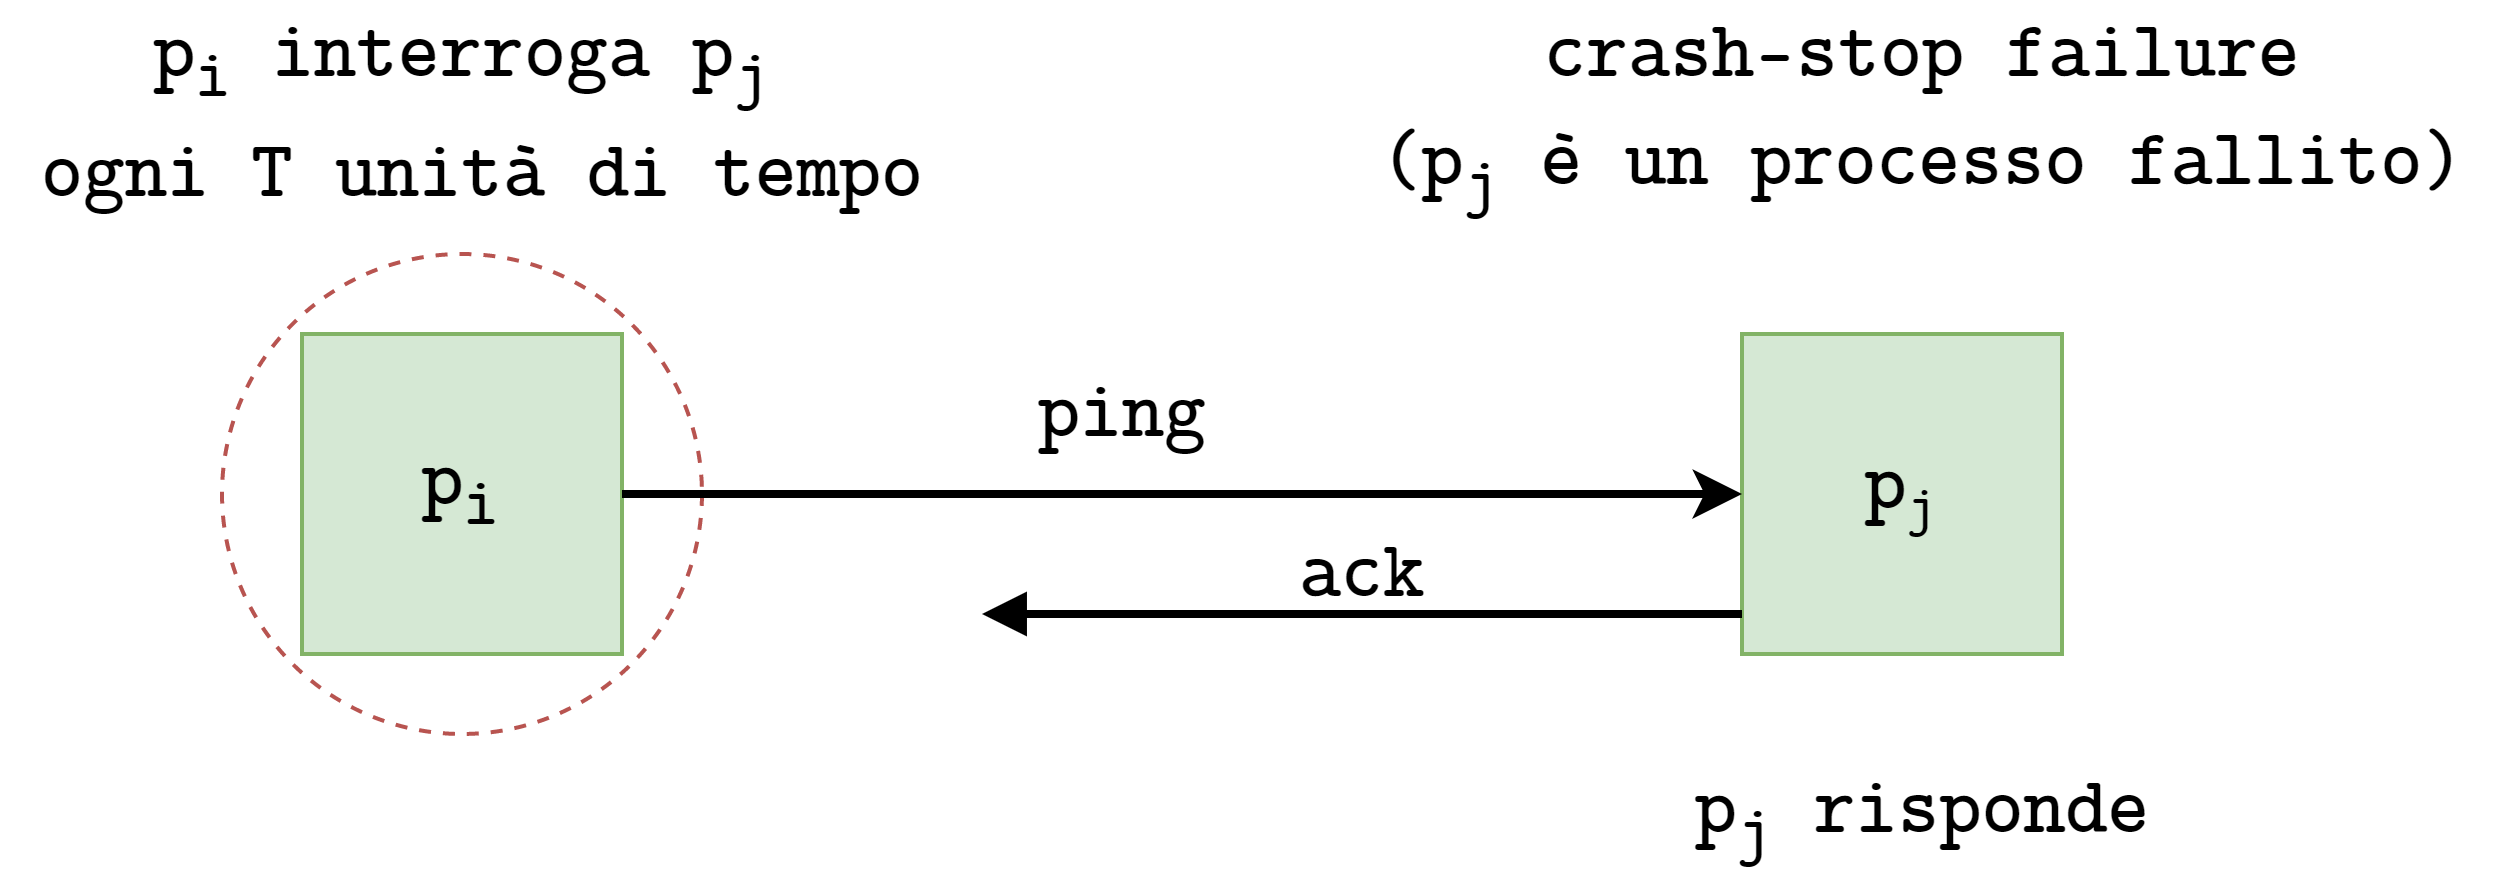
\includegraphics[width=7cm]{./Images/cap2/2.20.png}
\end{figure}

Una nuova astrazione, chiamata \textbf{accrual failure detector}, promuove flessibilità ed espressività operando con un livello di sospetto $\Phi$ su una scala continua, invece di tradizionali informazioni di natura booleana (fiducia vs sospetto).

In parole povere, questo valore $\Phi$ rappresenta il grado di certezza che un corrispondente processo monitorato si è arrestato in modo anomalo. Se il processo si blocca effettivamente, è garantito che il valore si accumuli nel tempo e tenda all'infinito.

Viene lasciato alle applicazioni il compito di impostare una soglia di sospetto appropriata in base ai propri requisiti di qualità del servizio: una soglia bassa è propensa a generare molti sospetti errati ma garantisce un rilevamento rapido in caso di incidente reale. Al contrario, una soglia alta genera meno errori ma richiede più tempo per rilevare gli arresti anomali effettivi.

Gli heartbeat arrivano dalla rete e il loro tempo di arrivo viene memorizzato nella finestra di campionamento. I campioni vengono utilizzati per stimare una certa distribuzione degli arrivi. Il tempo dell'ultimo arrivo T\textsubscript{last}, il tempo attuale e la distribuzione stimata vengono utilizzate per calcolare il valore corrente di $\Phi$. Le applicazioni poi attivano sospetti in base ad una certa soglia, o eseguono alcune azioni in funzione di $\Phi$.

\subsubsection{REALIZZAZIONI CONCRETE}
Nelle realizzazioni concrete di failure detector, sono possibili tre diversi approcci:
\begin{itemize}
    \item \textbf{centralizzato}: semplice da realizzare ed in grado di avere una completa visione del sistema, ma p\textsubscript{i} diventa una criticità (Single Point of Failure);
    \item \textbf{ad anello}: più complesso da realizzare, non presenta un nodo critico, ma è vulnerabile a possibili problemi sulla rete;
    \item \textbf{distribuito}: una soluzione che tollera maggiormente problemi di processi e di rete ma genera un forte carico di rete e consumo energetico. Una realizzazione più efficiente dell'approccio distribuito si basa sul gossiping.
\end{itemize}

\begin{figure}[ht]
    \centering
    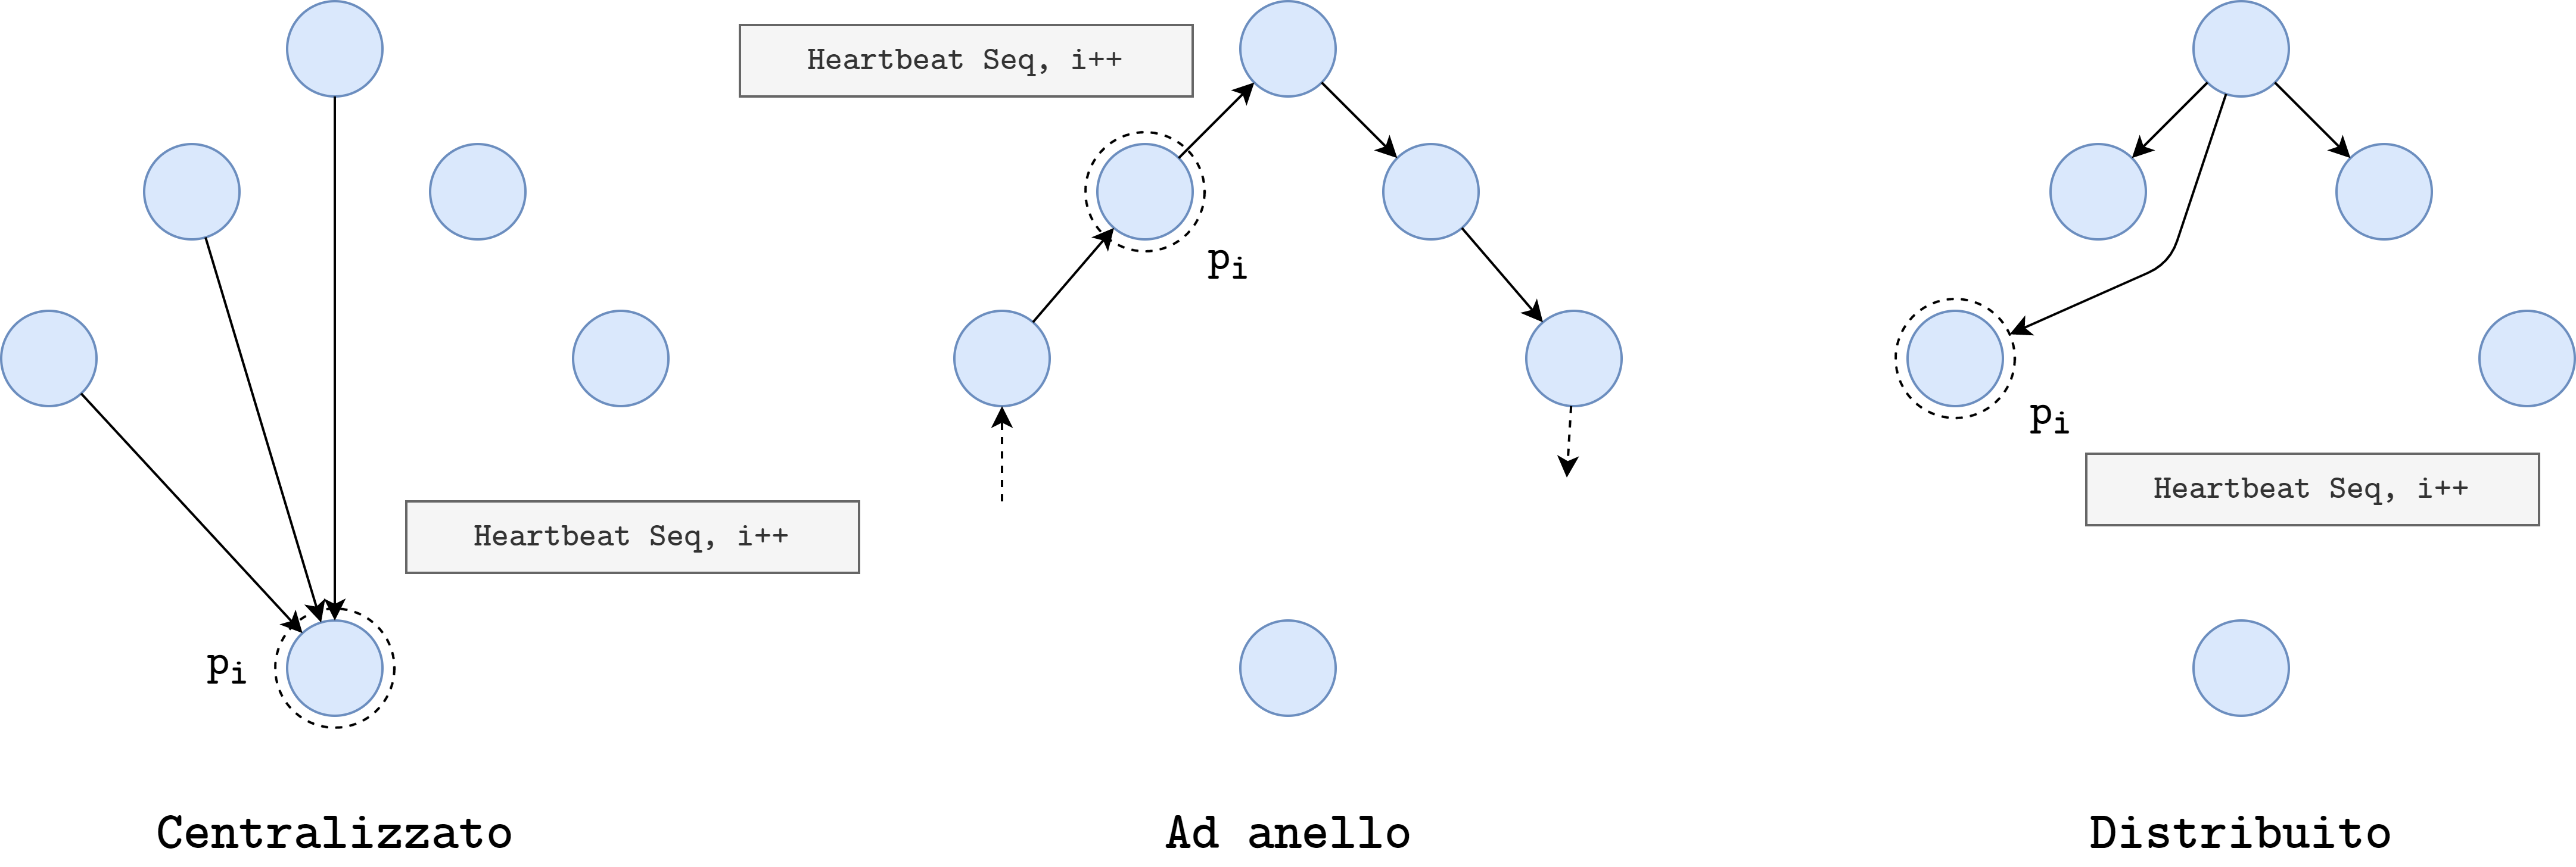
\includegraphics[width=10cm]{./Images/cap2/2.21.png}
\end{figure}

Il funzionamento dell'algoritmo è il seguente:
\begin{enumerate}
    \item Ogni processo mantiene un elenco di membri;
    \item Ogni processo incrementa periodicamente il proprio contatore di heartbeat;
    \item Ogni processo invia per mezzo del gossiping la sua lista di membri;
    \item Al ricevimento, gli heartbeat vengono uniti e l'ora locale viene aggiornata.
\end{enumerate}
Il tempo che un heartbeat impiega a propagarsi e a raggiungere tutti i processi del sistema con alta probabilità è $O(log(n))$. Lo schema è molto robusto contro gli errori: anche se un gran numero di processi si blocca, la maggior parte o tutti i processi rimanenti ricevono comunque tutti gli heartbeat.

Se l'heartbeat non è aumentato per più di T\textsubscript{fail} secondi, il processo corrispondente viene considerato non corretto, con T\textsubscript{fail} solitamente impostato su $O(log(n))$.

È lecito interrogarsi sull'effettiva utilità dei failure detector, infatti i FD inaffidabili possono generare falsi positivi (quindi essere inaccurati) e falsi negativi (essere incompleti), mentre i FD affidabili richiedono che il sistema sia sincrono (e pochi sistemi reali lo sono). Tuttavia i failure detector aiutano a comprendere la natura dei fallimenti in un sistema distribuito. Qualsiasi sistema reale progettato per gestire i fallimenti deve poterli rilevare, anche se maniera imperfetta.

\subsubsection{CONSENSO CON FAILURE DETECTOR}
Alcuni sistemi reali utilizzano FD \textit{"affidabili da progetto"} per raggiungere il consenso. I processi si accordano sull'indicare un processo \textit{p} come Failed se \textit{p} non risponde per più di un certo tempo nominale massimo, anche in un sistema asincrono. In realtà \textit{p} potrebbe non essere fallito, ma i rimanenti processi agiscono come se lo fosse: fanno diventare \textit{p fail-silent}, scartando tutti i messaggi che ricevono da esso. Ciò equivale a trasformare un sistema asincrono in un sistema sincrono. La tecnica è usata ad esempio in ISIS, il toolkit di comunicazione di gruppo per la programmazione distribuita realizzato dalla Cornell University.

\vspace{5mm}

Un altro approccio consiste nell'usare failure detectors inaffidabili. Il consenso viene raggiunto consentendo ai processi Suspected di agire come corretti e partecipare alla decisione, anziché escluderli. Chandra e Toueg hanno dimostrato che il consenso può essere raggiunto, anche in un sistema asincrono e usando detectors inaffidabili, se il numero di processi falliti non eccede N/2 e la comunicazione è affidabile. Il più debole failure detector che può essere usato allo scopo è un \textbf{eventually weak failure detector}.

Chandra e Toueg inoltre hanno dimostrato che in un sistema asincrono non è possibile implementare un \textit{eventually weak failure detector} solo attraverso scambio di messaggi, tuttavia un detector adattivo con timeout variabili va bene in molti casi pratici.

\section{Consistenza dei dati}
È una delle caratteristiche critiche di un sistema distribuito, principalmente perchè l'accesso spesso avviene a dati condivisi da più processi: i protocolli di locking su operazioni di lettura/scrittura limitano fortemente la concorrenza. Inoltre se si consentono accessi concorrenti su diverse repliche, migliorano le prestazioni e l'affidabilità.

Tuttavia, la replicazione comporta la necessità di mantenere la consistenza:
\begin{itemize}
    \item le modifiche ad una replica devono essere eseguite su tutte le altre repliche;
    \item bisogna tener conto di come e quando effettuare le modifiche mantenendo accettabili le prestazioni.
\end{itemize}
L'idea è quella di implementare la comunicazione con operazioni di \texttt{read}/\texttt{write} in uno spazio virtuale condiviso, senza usare primitive di \texttt{send} e \texttt{receive}, che sono implementate da DSM Manager.

Blockchain viene utilizzato in contesti che vogliono la consistenza dei dati in ambito distribuito, infatti spesso in un sistema distribuito le informazioni vengono replicate in più sottosistemi per aumentare le prestazioni. 

\subsection{Modelli di consistenza}
Sia $s_{i}$ il numero di operazioni da parte del processo $P_{i}$:
ci sono $\frac{(s_{1} + s_{2} + ... + s_{n})!}{s_{1}! s_{2}! ... s_{n}!}$ alternanze possibili, ma quante di queste sono permesse?

Un modello di consistenza è un contratto tra i processi e l'archivio di dati distribuito: se i processi rispettano un certo insieme di regole, l'archivio conterrà valori corretti. Processi concorrenti possono aggiornare simultaneamente un archivio di dati.

Gli accessi in lettura e in scrittura richiedono un tempo finito, ma sono operazioni diverse operate su processori diversi, che si possono sovrapporre nel tempo. Bisogna garantire che le operazioni conflittuali siano eseguite sulle varie repliche con un ordinamento che abbia una chiara semantica, ovvero:
\begin{itemize}
    \item conflitto \texttt{read-write}: una lettura e una scrittura concorrenti sullo stesso dato;
    \item conflitto \texttt{write-write}: due scritture concorrenti sullo stesso dato.
\end{itemize}
Il requisito generale è che una \texttt{read} restituisca il valore scritto dalla \texttt{write} più recente. La dicitura \textit{"più recente"} è ambigua in presenza di repliche e accessi concorrenti: il modello di consistenza specifica come viene determinata o definita la \texttt{write} più recente e rispetto a chi. Esistono quindi diversi modelli di consistenza:
\begin{itemize}
    \item Modelli di consistenza \textbf{data-centrici}: si occupano di fornire una vista di un archivio di dati consistente a livello di sistema;
    \item Modelli di consistenza \textbf{client-centrici}: si occupano di fornire una vista di un archivio di dati consistente a livello di un singolo client. Sono più veloci, ma meno accurati dei modelli data-centrici.
\end{itemize}

\subsection{Strict Consistency: modello ideale}
Corrisponde alla nozione di correttezza nel modello di Von Neumann monoprocessore: qualsiasi \texttt{read} su un dato \textit{x} restituisce un valore corrispondente al risultato più recente della \texttt{write} su \textit{x}, secondo un tempo globale.
\begin{itemize}
    \item \texttt{write\textsubscript{i}(x)a}: scrittura di \textit{P\textsubscript{i}} sul dato \textit{x} con valore scritto \textit{a}
    \item \texttt{read\textsubscript{i}(x)b}: lettura di \textit{P\textsubscript{i}} sul dato \textit{x} con valore scritto \textit{b}
\end{itemize}

\begin{figure}[ht]
    \centering
    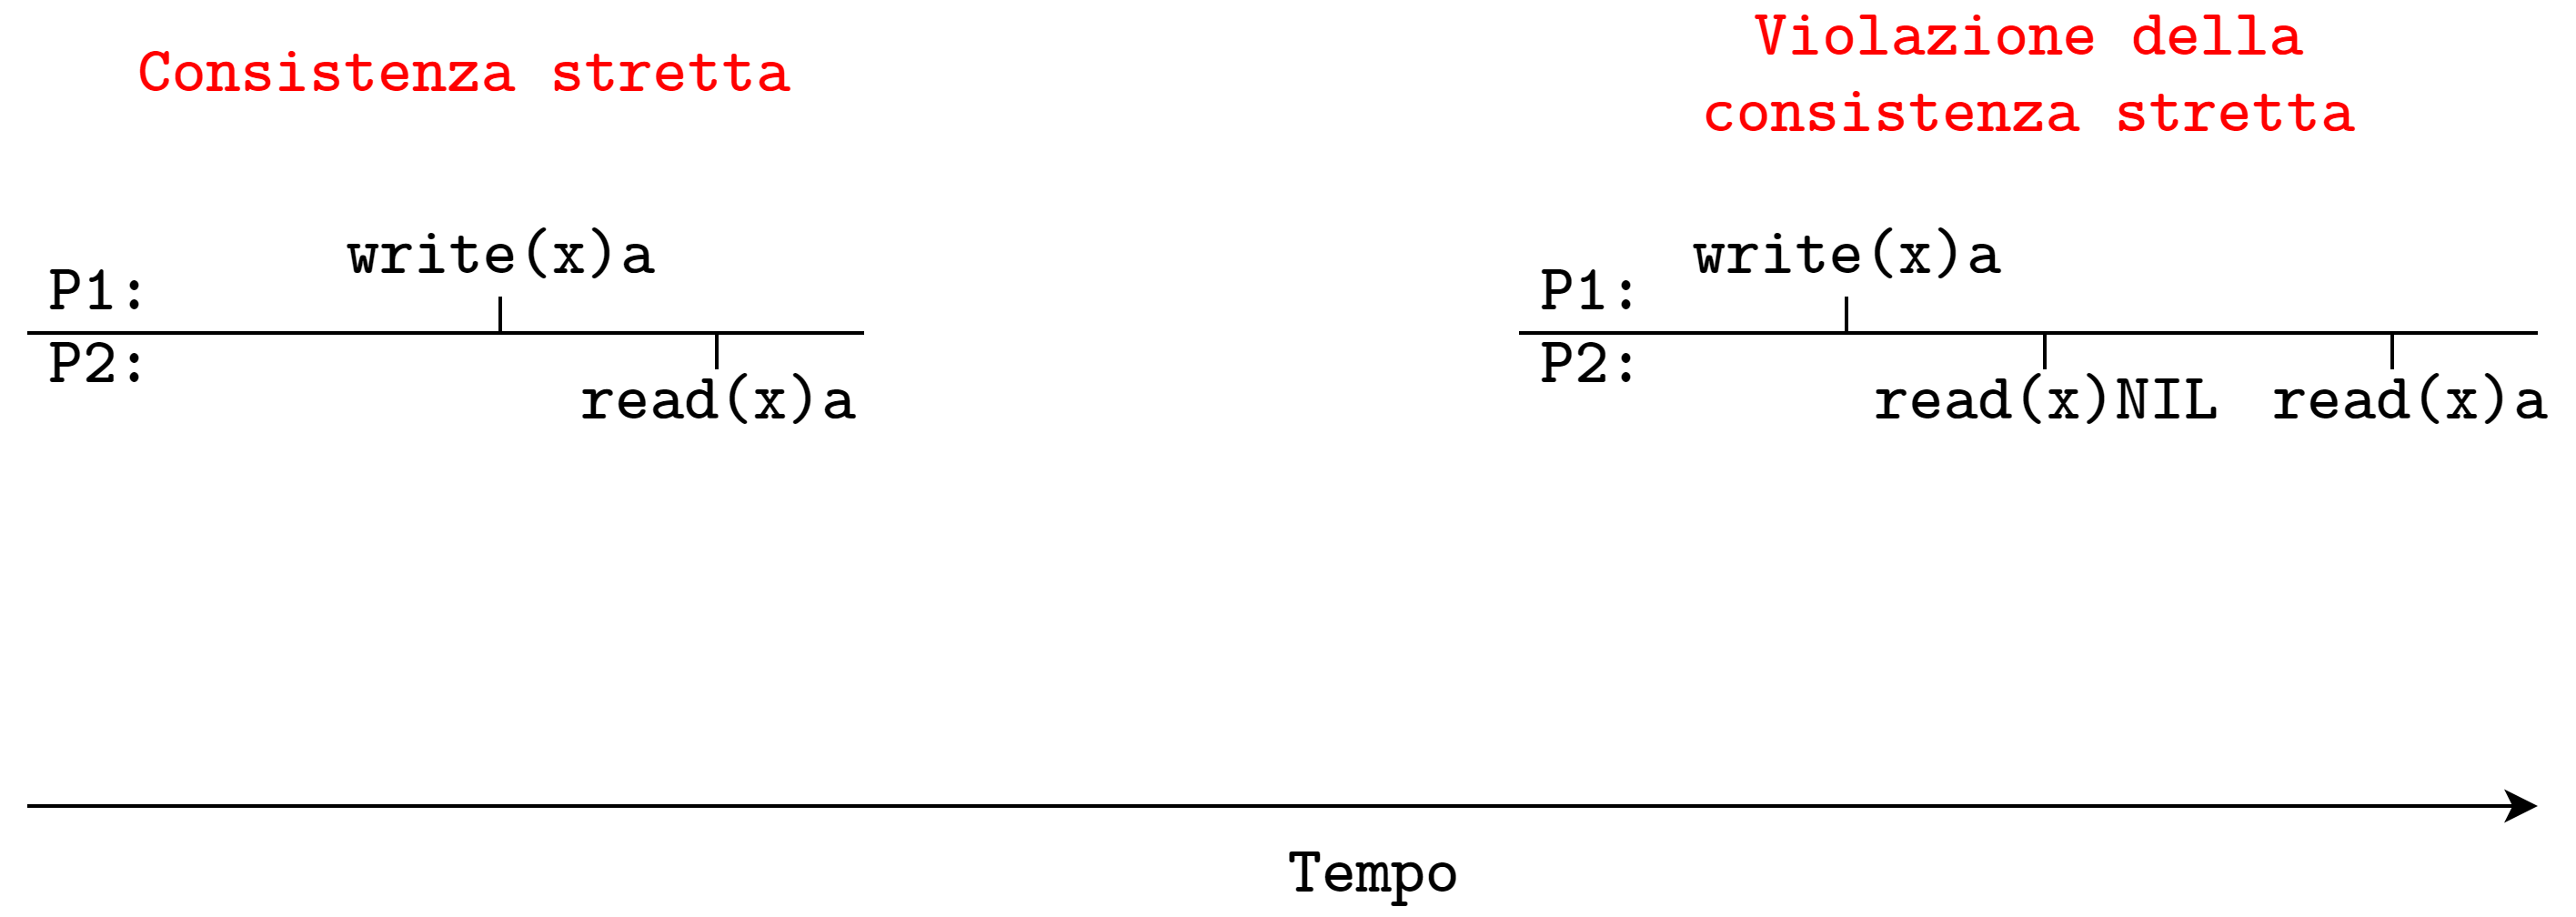
\includegraphics[width=10cm]{./Images/cap2/2.22.png}
\end{figure}

In questo modello la \texttt{write} viene vista istantaneamente da tutti i processi, e non c'è alcuna ambiguità sul più recente. Tuttavia richiede un tempo globale, quindi non è attuabile su un sistema distribuito, ma è possibile rilassare i vincoli di consistenza introducendo i concetti di \textbf{linearizzabilità} e \textbf{consistenza sequenziale}.

\subsection{Consistenza linearizzabile}
Tutte le operazioni ricevono un timestamp globale usando un clock sincronizzato. Linearizzabilità: il risultato di una qualunque esecuzione è uguale a quello ottenuto nel caso in cui:
\begin{itemize}
    \item le operazioni di tutti i processi sono eseguite in qualche ordine sequenziale;
    \item le operazioni di ogni singolo processo nella sequenza sono fatte nello stesso ordine indicato dal suo programma;
    se \textit{ts\textsubscript{OP1}(x) < ts\textsubscript{OP2}(y)} allora \textit{OP1(x)} deve precedere \textit{OP2(y)} nella sequenza.
\end{itemize}
Requisito real-time: le operazioni appaiono come se fossero eseguite istantaneamente su ogni nodo.

\begin{figure}[ht]
    \centering
    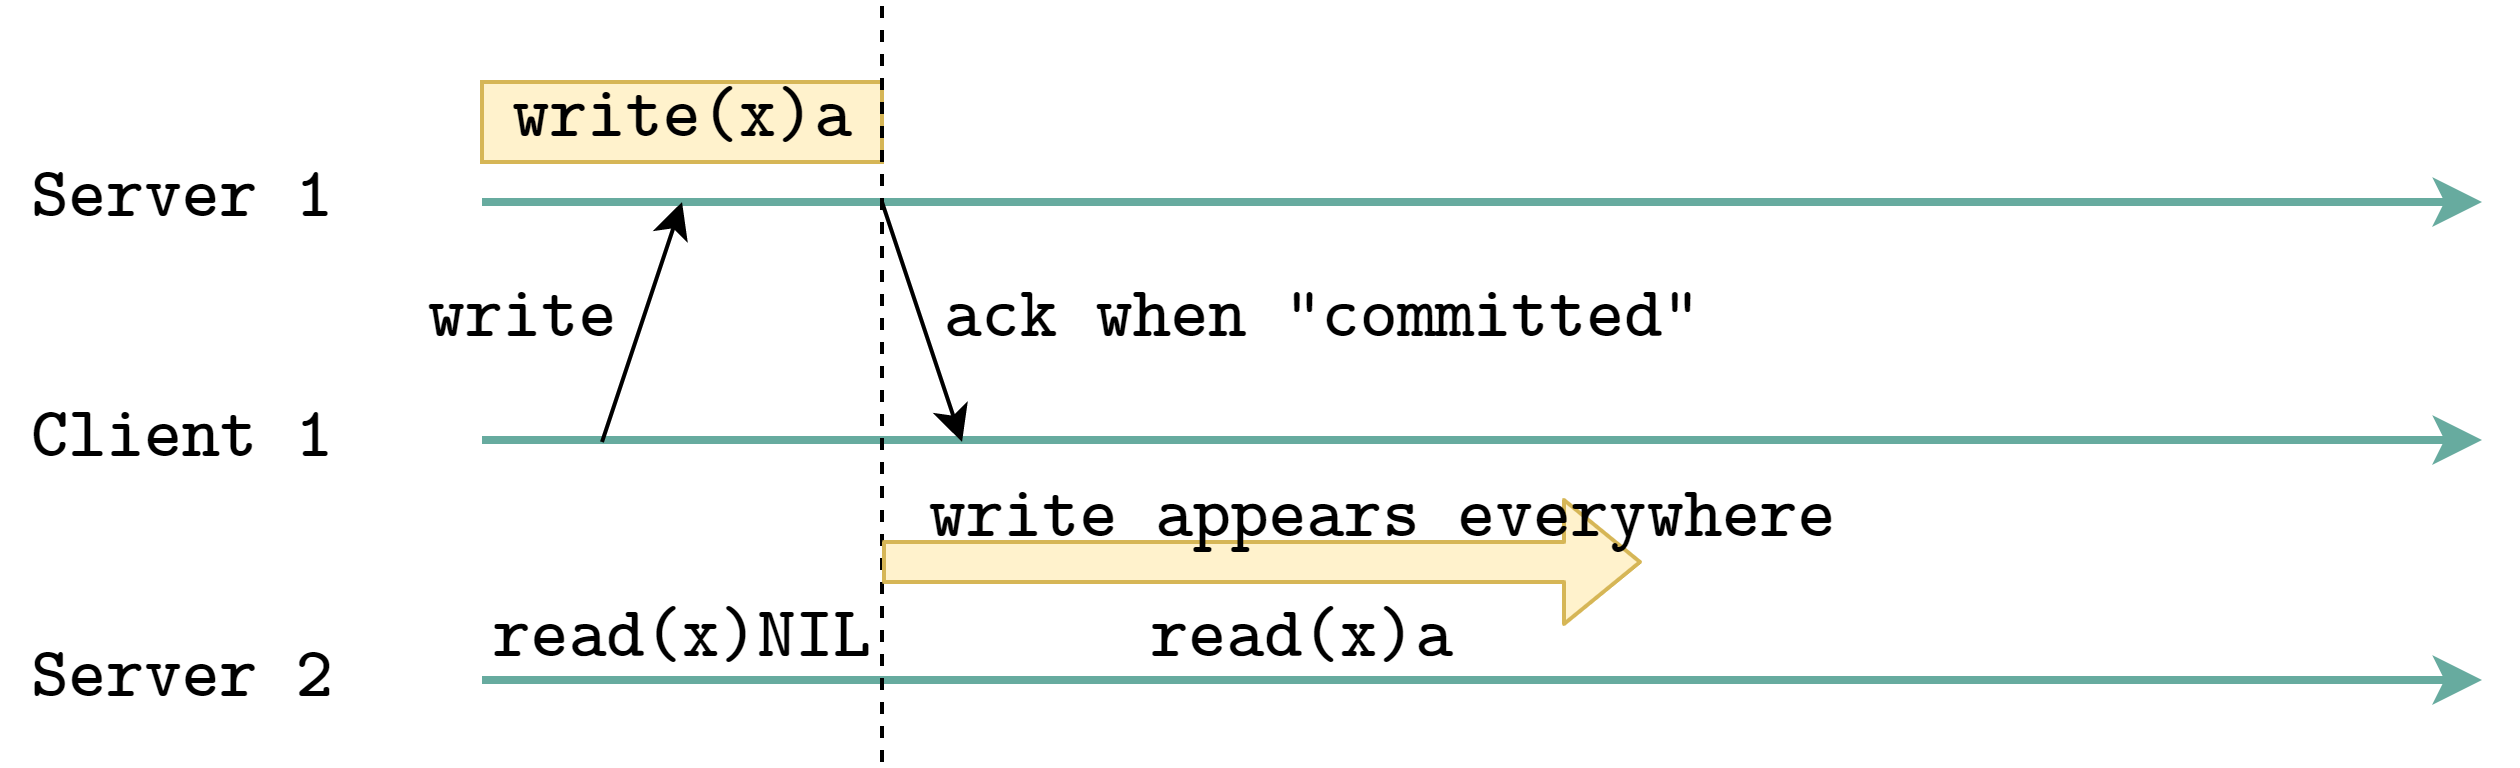
\includegraphics[width=10cm]{./Images/cap2/2.23.png}
\end{figure}

La linearizzabilità non prescrive uno specifico ordine per le operazioni che non si sovrappongono: si può implementare qualsiasi strategia di ordinamento purché ci sia un singolo ordinamento per le operazioni che si sovrappongono.

\vspace{5mm}

Una sequenza \textit{seq} di eventi <invocazione,risposta> è linearizzabile se esite una permutazione \textit{seq'} di coppie di eventi adiacenti che soddisfa i seguenti requisiti:
\begin{enumerate}
    \item Per ogni variabile \textit{v}, la proiezione di \textit{seq'} su \textit{v} è tale che ogni \texttt{read} (coppia di eventi adiacenti <invocazione,risposta>) restituisce l'esito della \texttt{write} più recente (coppia di eventi adiacenti <invocazione,risposta>) che l'ha immediatamente preceduta.
    
    Ogni processore vede una sequenza comune \textit{seq'} dove ogni lettura restituisce il valore della scrittura più recente.
    \item Se l'evento risposta di \textit{OP1} occorre prima dell'evento invocazione di \textit{OP2} nella sequenza \textit{seq}, allora \textit{OP1} (coppia di eventi adiacenti <invocazione,risposta>) occorre prima di \textit{OP2} (coppia di eventi adiacenti <invocazione,risposta>) anche in \textit{seq'} (ossia l'ordine temporale delle operazioni non sovrapposte in \textit{seq} deve essere preservato in \textit{seq'}).
    
    L'ordinamento comune \textit{seq'} rispetta l'ordinamento globale, \textit{seq'} preserva l'ordine delle operazioni non sovrapposte.
\end{enumerate}

La linearizzabilità si può realizzare ma è molto costosa: tutti i processori devono convenire su un ordinamento comune, occorre simulare una scala temporale globale e la linearizzabilità richiede il \textit{total ordering}, che a sua volta può essere implementato con il broadcast.

\subsection{Consistenza sequenziale}
Primo modello più debole della linearizzabilità, proposto da Lamport e basato su \textit{logical time}.

Il risultato di una qualunque esecuzione è uguale a quello ottenuto se le operazioni di \texttt{read} e \texttt{write} da parte di tutti i processi sull'archivio di dati fossero eseguite in qualche ordine sequenziale e le operazioni di ogni singolo processo apparissero in questa sequenza nell'ordine specificato dal suo programma. Quando i processi sono in esecuzione concorrente, qualunque alternanza di operazioni è accettabile, ma tutti i processo vedono la stessa alternanza di operazioni. Due operazioni che non si sovrappongono, anche se riguardano dati diversi, possono apparire in ordine inverso, purché sia lo stesso ordine per tutti.

\vspace{5mm}

Formalmente, una sequenza \textit{seq} di eventi <invocazione,risposta> è sequenzialmente consistente se esiste una permutazione \textit{seq'} di coppie di eventi adiacenti che soddisfa i seguenti requisiti:
\begin{enumerate}
    \item Per ogni variabile \textit{v}, la proiezione di \textit{seq'} su \textit{v} è tale che ogni \texttt{read} (coppia di eventi adiacenti <invocazione,risposta>) restituisce l'esito della \texttt{write} più recente (coppia di eventi adiacenti <invocazione,risposta>) che l'ha immediatamente preceduta.
    
    Questa condizione è la stessa della linearizzabilità.
    \item Se l'evento di risposta a \textit{OP1} in \textit{P\textsubscript{i}} occorre prima dell'evento invocazione di \textit{OP2} in \textit{P\textsubscript{i}} nella sequenza \textit{seq}, allora \textit{OP1} (coppia di eventi adiacenti <invocazione,risposta>) occorre prima di \textit{OP2} (coppia di eventi adiacenti <invocazione,risposta>) anche in \textit{seq'} (ossia l'ordine temporale delle operazioni non sovrapposte in \textit{seq} deve essere preservato in \textit{seq'}).
    
    L'ordinamento comune \textit{seq'} deve rispettare solo l'ordinamento locale, cioè \textit{seq'} non deve preservare l'ordine delle operazioni non sovrapposte eseguite da processi differenti.
\end{enumerate}
Nell’esempio seguente P\textsubscript{2} vede 0 perché la \texttt{write} è stata fatta su un altro nodo. Dopo la vede perché è contemporanea. La consistenza sequenziale è piu debole della linrealizzabilità quindi se non c’è la prima sicuramente non c’è la seconda.
\clearpage

\begin{figure}[t]
    \centering
    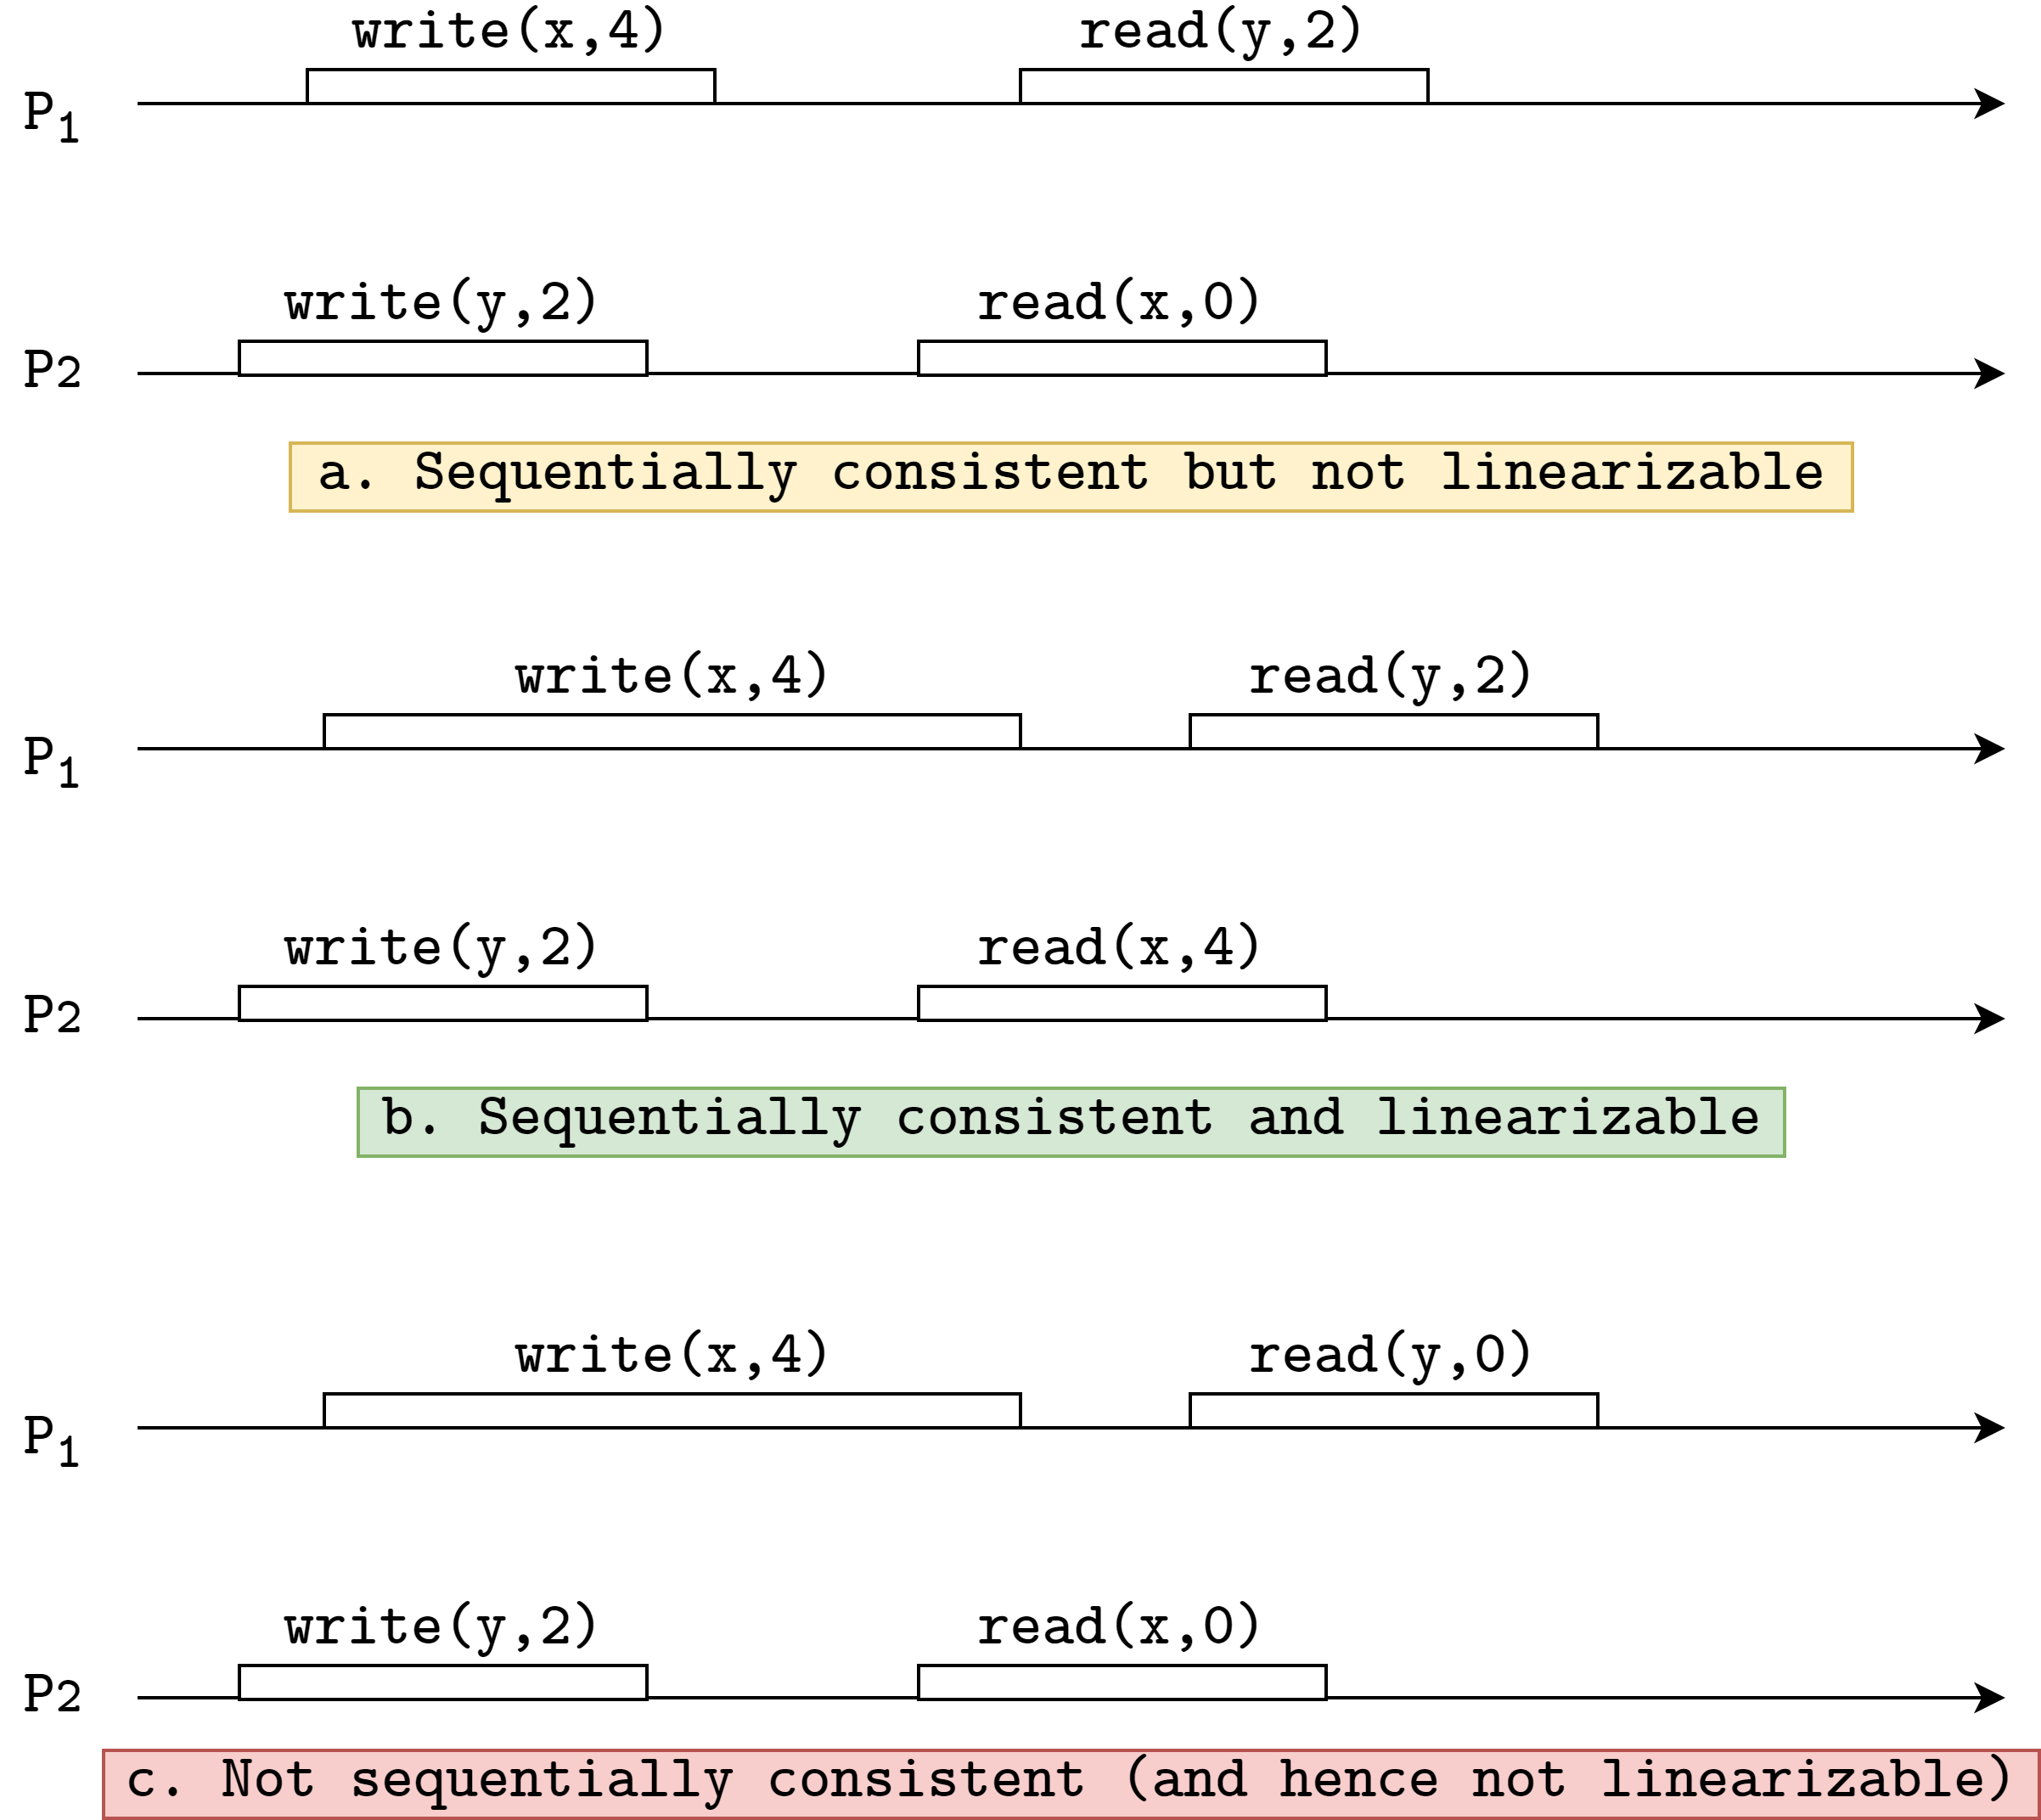
\includegraphics[width=10cm]{./Images/cap2/2.24.png}
\end{figure}

\subsection{Consistenza causale}
Relazione di causalità:
\begin{itemize}
    \item \textbf{Local order}: l'ordine locale degli eventi definisce l'ordine causale.
    \item \textbf{Inter-process order}: una \texttt{write} precede causalmente una \texttt{read} eseguita da un altro processo se la \texttt{read} restituisce il valore scritto della \texttt{write}. 
    \item \textbf{Transitive closure}: la chiusura transitiva delle due relazioni precedenti definisce l'ordine causale globale. 
\end{itemize}

Per la consistenza causale, solo le \texttt{write} correlate causalmente devono essere viste nello stesso ordine. Operazioni di \texttt{write} che sono potenzialmente in relazione di causa/effetto devono essere viste da tutti i processi nello stesso ordine. Operazioni di \texttt{write} concorrenti possono essere viste in ordine differente da processi differenti. Indebolisce la consistenza sequenziale, perché distingue tra operazioni in relazione causale e quelle che non lo sono.
\clearpage

\begin{figure}[ht]
    \centering
    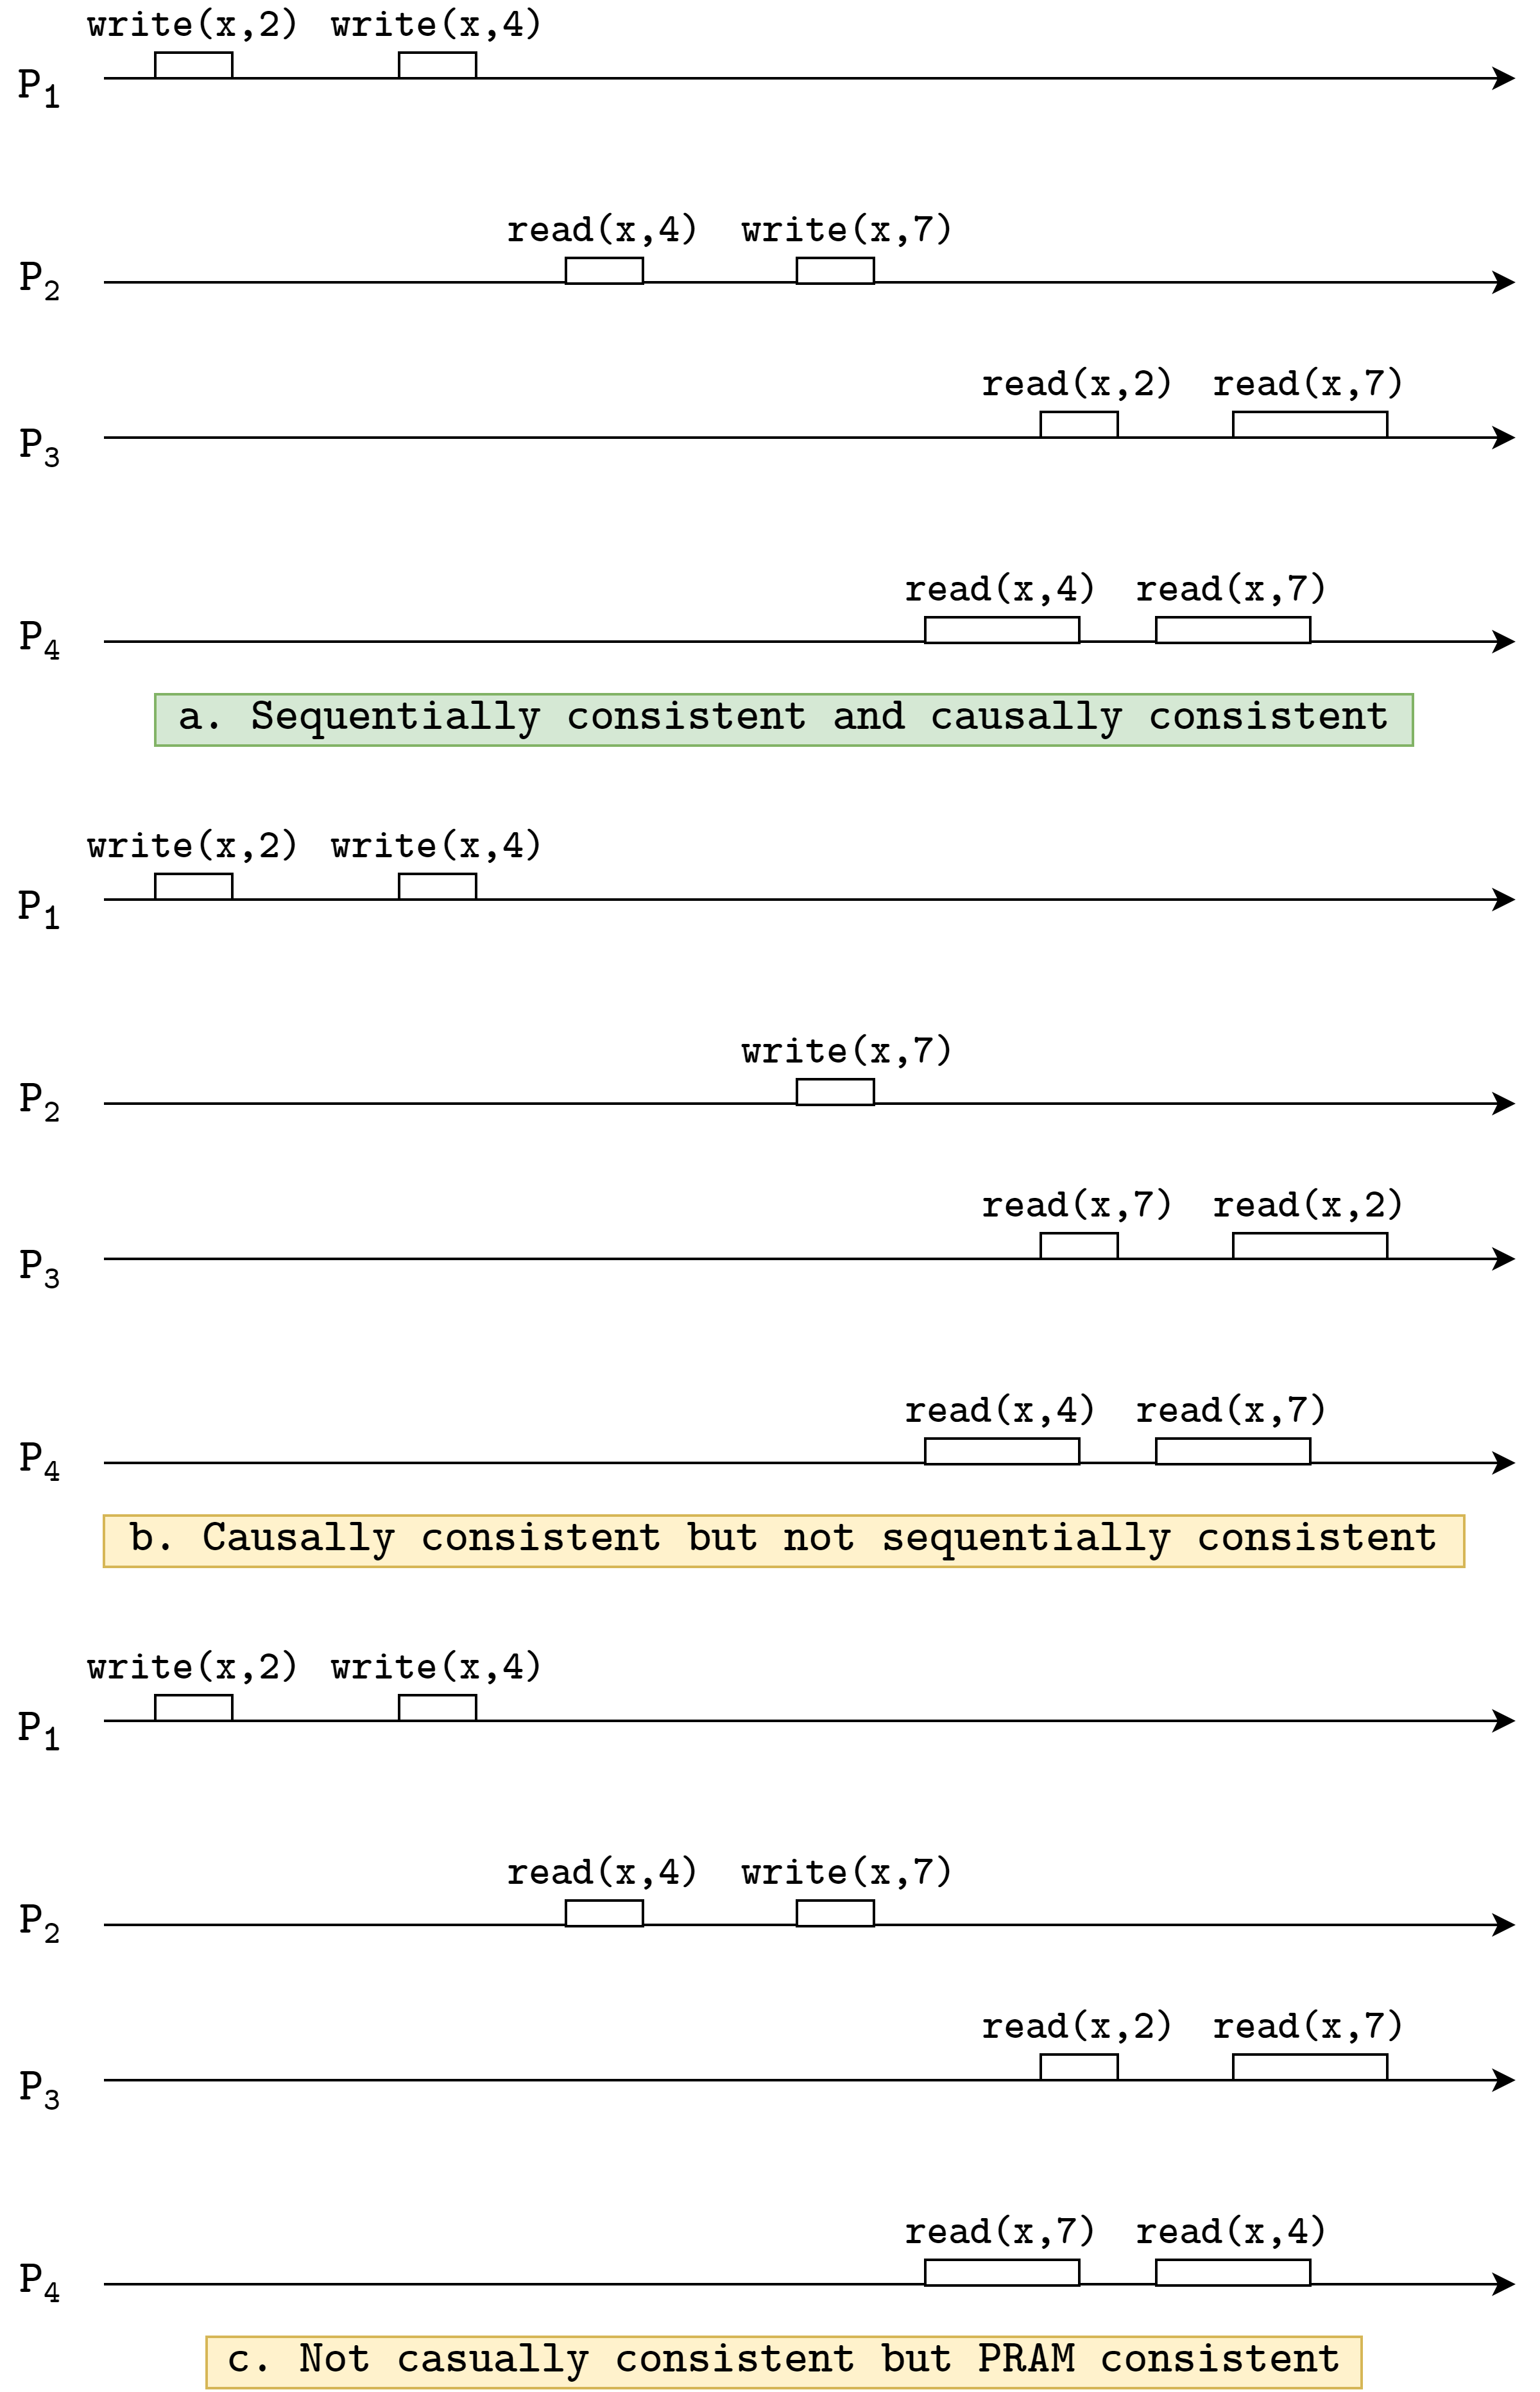
\includegraphics[width=10cm]{./Images/cap2/2.25.png}
\end{figure}

% Please add the following required packages to your document preamble:
% \usepackage[table,xcdraw]{xcolor}
% If you use beamer only pass "xcolor=table" option, i.e. \documentclass[xcolor=table]{beamer}
\begin{table}[ht]
\centering
\begin{tabular}{ll}
\rowcolor[HTML]{EFEFEF} 
\multicolumn{1}{c}{\cellcolor[HTML]{EFEFEF}\textbf{Consistenza}} & \multicolumn{1}{c}{\cellcolor[HTML]{EFEFEF}\textbf{Descrizione}}                                                                                                                     \\
Stretta                                                          & \begin{tabular}[c]{@{}l@{}}Tutti i processi vedono gli accessi condivisi nello\\ stesso ordine assoluto di tempo\end{tabular}                                                        \\
Linearizzabile                                                   & \begin{tabular}[c]{@{}l@{}}Tutti i processi vedono gli accessi condivisi nello\\ stesso ordine: gli accessi sono ordinati in base ad un\\ timestamp globale (non unico)\end{tabular} \\
Sequenziale                                                      & \begin{tabular}[c]{@{}l@{}}Tutti i processi vedono gli accessi condivisi nello\\ stesso ordine; gli accessi non sono ordinati\\ temporalmente\end{tabular}                           \\
Causale                                                          & \begin{tabular}[c]{@{}l@{}}Tutti i processi vedono gli accessi condivisi correlati\\ causalmente nello stesso ordine\end{tabular}                                                   
\end{tabular}
\end{table}

\subsection{Consistenza con sincronizzazione}
Permette di raggruppare le operazioni e le condizioni di consistenza sono applicate solo a istruzioni di sincronizzazione; le istruzioni non di sincronizzazione possono essere eseguite in ordine diverso dai vari processori.

Un esempio è dato dalla consistenza debole:
\begin{itemize}
    \item Tutte le \texttt{write} sono propagate agli altri processi, e tutte le \texttt{write} fatte altrove sono riportate localmente, all'occorrenza dell'istruzione di sincronizzazione.
    \item Gli accessi a variabili di sincronizzazione sono sequenzialmente consistenti.
    \item L'accesso a variabili di sincronizzazione non è permesso finché tutte le precedenti \texttt{write} non sono state completate su tutte le copie.
    \item Nessuna \texttt{read} o \texttt{write} su un dato è permessa finché non siano stati eseguiti tutti i precedenti accessi sulle variabili di sincronizzazione.
\end{itemize}
Le variabili di sincronizzazione sono due: \textbf{acquire} e \textbf{release}:
\subsubsection{CONSISTENZA RELEASE}
\begin{itemize}
    \item \textbf{Acquire} indica l'ingresso nell SC. Tutte le \texttt{write} dagli altri processi devono riglettersi localmente all'occorrenza di questa istruzione.
    \item \textbf{Release} indica l'uscita dalla SC. Tutti gli aggiornamenti fatti localmente devono essere propagati alle repliche.
\end{itemize}
\textbf{Acquire} e \textbf{release} sono definibili su un sottoinsieme delle variabili. Si parla di consistenza \textit{lazy release} quando gli aggiornamenti sono propagati on demand.

\subsubsection{CONSISTENZA ENTRY}
Ogni variabile ordinaria condivisa è associata ad una variabile di sincronizzazione. All'atto dell'\textbf{acquire} su una variabile di sincronizzazione, è eseguito l'accesso soltanto alle variabili ordinarie protette da quella variabile di sincronizzazione.

\subsection{Teorema CAP}
In presenza di un partizionamento, per mantenere la consistenza, bisogna bloccare il sistema rendendolo non disponibile. Se venissero servite infatti le richieste dalle due partizioni, ci sarebbe l'inconsistenza anche se il sistema sarebbe disponibile.
Il teorema CAP formalizza questa situazione. Proposto da E. Brewer nel 2000 e dimostrato da S. Gilbert e N. Lynch nel 2002, afferma che:

\vspace{5mm}

\begin{center}
    \textit{"Ogni sistema in rete che condivide dati può avere in un dato istante al più due delle tre proprietà desiderabili:}
    \begin{itemize}
        \item \textit{\textbf{Consistency (C)}: avere una copia aggiornata dei dati;}
        \item \textit{\textbf{Availability (A)}: disponibilità dei dati anche in presenza di fallimenti;}
        \item \textit{\textbf{Tolerance to network partitions (P)}: le proprietà del sistema permangono anche in caso di partizionamenti."}
    \end{itemize}
\end{center}

\vspace{5mm}

Se la priorità è la consistenza, si rinuncia all'availability (sistema CP). Se invece la priorità è l'availability, si rinuncia alla consistenza (sistema AP), usando un modello di consistenza più debole (eventual consistency).

Quando si adottano sistemi CP e AP, lo sviluppatore deve sapere cosa offre il sistema:
\begin{itemize}
    \item \textbf{sistema CP}: il sistema può non essere disponibile ad eseguire una \texttt{write}. Lo sviluppatore deve gestire il fallimento di una \texttt{write} causato dall'eventuale indisponibilità del sistema.
    \item \textbf{sistema AP}: il sistema può accettare sempre una \texttt{write}, ma sotto certe condizioni una \texttt{read} non riporterà il risultato della \texttt{write} più recente. Lo sviluppatore deve decidere se il client può richiedere sempre l'accesso all'ultimo aggiornamento.
\end{itemize}

\subsection{Eventual Consistency}
In un archivio di dati distribuito caratterizzato da mancanza di conflitti \texttt{write/write} o comunque di facile soluzione in caso di conflitto, e con forte prevalenza di letture rispetto alle scritture, si adotta spesso un modello di consistenza rilassato, detto \textbf{consistenza finale} (eventual consistency). Questa garantisce che se non si verificano aggiornamenti, tutte le repliche (distribuite geograficamente) diventano gradualmente consistenti entro una finestra temporale (detta inconsistency window). In assenza di failure, la dimensione della inconsistency window dipende da ritardi di comunicazione, carico del sistema e numero di repliche.

I vantaggi di questa implementazione sono dati dal fatto che è semplice da realizzare e poco costosa; tuttavia c'è uno svantaggio: se l'utente accede a repliche diverse in un breve intervallo di tempo, potrebbe accedere a dati non aggiornati: in tal caso occorre risolvere il conflitto (\textit{reconciliation}).

\vspace{5mm}

L'Eventual consistency è un modello di consistenza spesso adottato nei sistemi distribuiti a larga scala, in particolare per servizi di storage e datastore NoSQL in ambito Cloud (Amazon S3, Apache, Dropbox, e qualche servizio Google).

C'è da dire però che il costo di garantire un maggior livello di consistenza ricade sullo sviluppatore dell'applicazione. Con la consistenza finale, può accadere che una \texttt{read} non restituisca il valore della \texttt{write} più recente: lo sviluppatore deve decidere se tale inconsistenza è accettabile per l'utente dell'applicazione.

\subsection{Risoluzione dei conflitti e ACID vs BASE}
Strategie per decidere come risolvere conflitti su copie divergenti a causa di aggiornamenti concorrenti.
Un approccio comune è quello del \textit{last writer wins} (come in Cassandra): etichettare i dati con orologi vettoriali per catturare la causalità tra diverse versioni dei dati.

Un'alternativa è demandare la risoluzione all'applicazione stessa (come in Amazon Dynamo) che invoca un gestore dei conflitti specificato dall'utente. Tipicamente la riconciliazione viene fatta a tempo di \texttt{read}.

\vspace{5mm}

ACID e BASE sono filosofie di design agli estremi opposti dello spettro \textit{consistency - availability}:

\textbf{ACID (Atomicity, Consistency, Isolation, Durability}:
\begin{itemize}
    \item Approccio tradizionale per garantire consistenza nei DBMS
    \item DMBS tramizionali (Postgres, MySQL) sono esempi di sistemi CP
    \item Approccio pessimistico: non scalabile quando bisogna gestire migliaia di terabyte di dati
\end{itemize}

\textbf{BASE (Basically Available, Soft state, Eventual consistency}:
\begin{itemize}
    \item Approccio ottimistico e per sistemi AP
    \item Basically available: il sistema è disponibile per la maggior parte del tempo, potrebbero esserci sottoinsiemi temporaneamente non disponibili
    \item Soft state: la persistenza è gestita dall'utente, che deve preoccuparsi di aggiornare i dati
    \item Eventualli consistent: il sistema prima o poi converge ad uno stato consistente
    \item Soft state ed eventual consistency sono tecniche che funzionano bene in presenza di partizionamenti, favorendo la disponibilità. È tipicamente adottato in database NoSQL
\end{itemize}

\subsection{Modelli user-centrici}
La consistenza in questi modelli è di quattro tipi diversi:
\begin{itemize}
    \item \textbf{monotonic-read} (read-after-read)
    \item \textbf{monotonic-write} (write-after-write)
    \item \textbf{read-your-writes} (read-after-write)
    \item \textbf{writes-follow-reads} (write-after-read)
\end{itemize}

L'obiettivo è fornire garanzie ad un singolo client relative alla consistenza degli accessi da parte di quel client ad un archivio di dati distribuito. Non viene data alcuna garanzia di consistenza relativamente agli accessi concorrenti da parte di altri client.

Alcune spiegazioni che potrebbero servire:
\begin{itemize}
    \item $x_{i}[t]$: versione di $x$ sulla copia locale $L_{i}$ al tempo $t$
    \item $WS(x_{i}[t])$: sequenza di operazioni di scrittura (Write Set) su $L_{i}$ che hanno portato come risultato a $x_{i}[t]$
    \item $WS(x_{i}[t_{1}]; x_{j}[t_{2}])$: le operazioni in $WS(x_{i}[t_{1}])$ sono state eseguite anche su $L_{j}$ in un tempo successivo $t_{2}$
    \item significa che $WS(x_{i}[t_{1}])$ è parte di $WS(x_{j}[t_{2}])$
    \item assumiamo che solo il processo proprietario dei dati possa modificarli (assenza di conflitti \texttt{write/write})
\end{itemize}

\subsubsection{MONOTONIC READ}
Se un processo legge il valore di un dato \textit{x}, qualunque successiva operazione di lettura su x da parte di quel processo restituirà sempre quello stesso valore o un valore più recente.

Ad esempio, leggere automaticamente gli aggiornamenti al proprio calendario personale da diverse repliche del servizio: la consistenza \textit{monotonic-read} garantisce all'utente di vedere tutti gli aggiornamenti, a prescindere dalla replica su cui avviene la lettura.

Un altro esempio è leggere senza modificare la posta in arrivo mentre ci si sposta: ogni volta che l'utente si connette ad una diversa replica del mail server, la replica carica tutti gli aggiornamenti relativi alla mailbox dell'utente dalla replica usata precedentemente.

\subsubsection{MONOTONIC WRITE}
Un'operazione di scrittura da parte di un processo su un dato \textit{x} viene completata prima di qualunque operazione di scrittura successiva su x da parte dello stesso processo. L'archivio garantisce di serializzare le scritture per il singolo client.

Ad esempio, mantenere versioni di file replicati nell'ordine corretto su ogni server, propagando la versione precedente sul server dove è installata la nuova versione.

\subsubsection{READ YOUR WRITES}
L'effetto di un'operazione di scrittura da parte di un processo su un dato \textit{x} sarà sempre visto da una successiva operazione di lettura di \textit{x} da parte dello stesso processo. È un caso speciale di consistenza causale per il singolo client.

Ad esempio, aggiornare la propria pagina web e garantire che il browser mostri la versione più recente anziché la copia in cache.

\subsubsection{WRITES FOLLOW READS}
Un'operazione di scrittura da parte di un processo su un dato \textit{x} che segue una precedente operazione di lettura di \textit{x} da parte dello stesso processo ha luogo sullo stesso valore di \textit{x} che è stato letto o su un valore più recente.

Ad esempio, vedere i commenti ad un articolo inserito in un \textit{newsgroup} solo se è stato visto l'articolo originale.


